\section{Heavy quark phenomenology and New Physics}
The top quark is a very interesting elementary particle of the \sm\ because of its high mass, which is comparable to the electroweak symmetry breaking scale. 
This fact makes top quark a subject of many New Physics theories. 
The measurements of the bottom quark properties, a partner of the top quark, have revealed a tension with \sm\ predictions. 
Many \bsm\ theories can modify heavy quark properties, therefore, precise measurements of heavy quark couplings are required for indirect searches of new particles and discrimination between various theories. 

This section of the thesis concentrates on the electroweak interaction of the top and bottom quarks, corresponding observables, heavy quark production at linear colliders and possible influence of New Physics.
%the higgs is tightly connected to the top quark via coupling that is proportional to the top mass
%The bottom quark is in the same doublet as top
%%%%%%%%%%%%%%%%%%%%%%%%%%%%%%%%%%%%%%%%%%%%%%
%%%%%%%%%%%%%%%%%%%%%%%%%%%%%%%%%%%%%%%%%%%%%%
%%%%%%%%%%%%%%%%%%%%%%%%%%%%%%%%%%%%%%%%%%%%%%
\subsection{Total cross section and forward-backward asymmetry}
%First, one needs to define the most convenient parametrization of coupling or form factors of interest, and then express the observable quantities in terms of defined form factors. 

At the electron-positron colliders the heavy quarks are mainly produced via $f\bar{f}X$ vertex, where $X$ stands for neutral vector bosons, photon or $Z^0$ boson.  The current at $f\bar{f}X$ vertex can be expressed via form factors $F$ as 
\begin{equation}
	\Gamma^{f\bar{f}X}_\mu (k^2,q,\bar{q}) = ie\{ \gamma_\mu (F^X_{1V}(k^2) + \gamma^5 F^X_{1A}(k^2)) - \frac{\sigma_{\mu\nu}(q-\bar{q})^\nu}{2m_f}(iF^X_{2V}(k^2) + \gamma^5 F^X_{2A}(k^2)) \},
\end{equation}
where $k^2= (q+\bar{q})^2$ is the four momentum squared of the exchanged vector boson, $q$ and $\bar{q}$ are the four vectors of the fermion $f$ and antifermion $\bar{f}$ and $m_f$ is the fermion mass. Further, $\gamma_\mu$ and $\gamma_5$ are the Dirac matrices, and $\sigma_{\mu\nu} = i/2(\gamma_\mu\gamma_\nu - \gamma_\nu\gamma_\mu)$.

The \sm\ values of the form factors $F$ are the following:
\begin{equation}
	F^{f\gamma}_{1V} = Q^{f}, \ F^{f\gamma}_{1A} = 0, \ F^{fZ}_{1V} = \frac{I^f - 2Q^f\sin^2\theta_W}{2\cos\theta_W\sin\theta_W}, \ F^{fZ}_{1A} = - \frac{I^f}{2\cos\theta_W\sin\theta_W},
    \label{formula:SMformFactors_3}
\end{equation}
and all $F_2$ factor are zero. In the expression \ref{formula:SMformFactors_3} $I^f$ is the weak isospin number, $I^t = 1/2$ for top and $I^b = -1/2$ for bottom quark and $q^f$ is an electric charge, $Q^t = 2/3$ and $Q^b = -1/3$.

The form factors are related to fermion couplings with left and right-handed helicity to $Z^0$ boson:
\begin{equation}
	g_L^Z = F_{1V}^Z - F_{1A}^Z, \  g_R^Z = F_{1V}^Z + F_{1A}^Z, 
    \label{formula:EWcouplings_3}
\end{equation}
the same relations are applied to the corresponding photon couplings $g^\gamma_L$.
%At the tree level, the \sm\ differential cross for the production
%of a fermion $f$ pair in $e^+e^-\to f\bar{f}$ at center-of-mass energy $\sqrt[]{s}$ can be written as

In case of the polarized beams, the fermion form factors can be expressed in terms of the helicity of the initial electrons:
\begin{eqnarray}
	\mathcal{F}^L_{ij} = - F^\gamma_{ij} +  \frac{-1/2 + \sin^2\theta_W}{\cos\theta_W\sin\theta_W}\frac{s}{s-M^2_Z+i\Gamma_ZM_Z}F^Z_{ij},\\
    \mathcal{F}^R_{ij} = - F^\gamma_{ij} +  \frac{\sin^2\theta_W}{\cos\theta_W\sin\theta_W}\frac{s}{s-M^2_Z+i\Gamma_ZM_Z}F^Z_{ij}    
\end{eqnarray}
where $i=1,2$ and $j=V,A$.
The first observable is the cross section for $f\bar{f}$ for electron beam polarization $I=L,R$ can be expressed in terms of these form factors:
\begin{equation}
	\sigma_I = 2\frac{4\pi\alpha^2}{3s}N_c\beta[(1+\frac{1}{2}\gamma^{-2})(\mathcal{F}^I_{1V})^2 + (\beta\mathcal{F}^I_{1A})^2+3\mathcal{F}^I_{1V}\mathcal{F}^I_{2V}+(1+\frac{1}{2}\gamma^{2})(\mathcal{F}^I_{2V})^2],
\end{equation}
where $\alpha$ is the electromagnetic running coupling, $N_c$ is a number of quark colors, $\beta$ and $\gamma$ are the velocity and the Lorentz factor of produced fermion, respectively. 
The total cross section can be measured knowing the number of accepted events $N$, selection efficiency $\epsilon$ and integrated luminosity $\mathcal{L}_I$
\begin{equation}
	\sigma_I = \frac{N}{\epsilon \mathcal{L}_I}.
    \label{formula:Xsection_3}
\end{equation}
The forward-backward asymmetry is an observable, which counts the difference between the number of events in the forward region and backward regions:
\begin{equation}
	A_{fb} = \frac{\sigma(cos\theta > 0) - \sigma(cos\theta < 0)}{\sigma(cos\theta > 0) + \sigma(cos\theta < 0)}.
\end{equation}
In case of polarized beams at $e^+e^-$ machines, it can be expressed as
\begin{equation}
	A_{fb}^I = \frac{-3\beta\mathcal{F}^I_{1A}(\mathcal{F}^I_{1V} + \mathcal{F}^I_{2V})}{2[(1+\frac{1}{2}\gamma^{-2})(\mathcal{F}^I_{1V})^2 + (\beta\mathcal{F}^I_{1A})^2+3\mathcal{F}^I_{1V}\mathcal{F}^I_{2V}+(1+\frac{1}{2}\gamma^{2})(\mathcal{F}^I_{2V})^2]}.
    \label{formula:AfbForm_3}
\end{equation}
This observable is sensitive to the axial form factor $\mathcal{F}^I_{1A}$, therefore the it is crucial to measure $A_{fb}^I$ precisely to reduce uncertainty on the corresponding form factors.

%single top
Another source of top quark production at linear colliders is the single top process. %which is shown in Fig. \ref{fig:singletop_3}. 
This process allows top quark production at 250\,GeV center-of-mass energy, but the study of the single top production is not included in the thesis. 

\subsubsection{New Physics influence}
The heavy quarks and the Higgs boson are often subject of \bsm\ deviations.
For example, supersymmetric extensions of the \sm\ predict different set of Higgs couplings to the up type and down type quarks. 
\bsm\ theories with additional weak bosons $Z'$ or $W'$ can have a mixing with the \sm\ bosons, which can modify the electroweak couplings of the heavy quarks. 
The extradimentional extensions of the \sm\ like Randall-Sundrum models are able to provide an explanation to the mass hierarchy, and have additional weak boson excitations. 

The possible compositness of heavy quarks can also leave an imprint on the their electroweak couplings, which is described by various technicolor theories.
The relative deviations of left-handed and right-handed couplings of the top quark are predicted by various BSM theories are shown in Fig.~\ref{fig:DeviationsTop}.
A precise measurement of the top coupling allows for identification of the particular BSM theory.  
The experiments with polarized beams have an advantage of detection of sign flip of the right-handed coupling $g_R^Z$, which can be produced by the Randall-Sundrum models with $Z^0$-$Z'$ mixing~\cite{bib:RSTOP}.
%
%Many \bsm\ models predict deviations on the heavy quark couplings to the Higgs and weak bosons.

\begin{figure}[h]
{\centering
    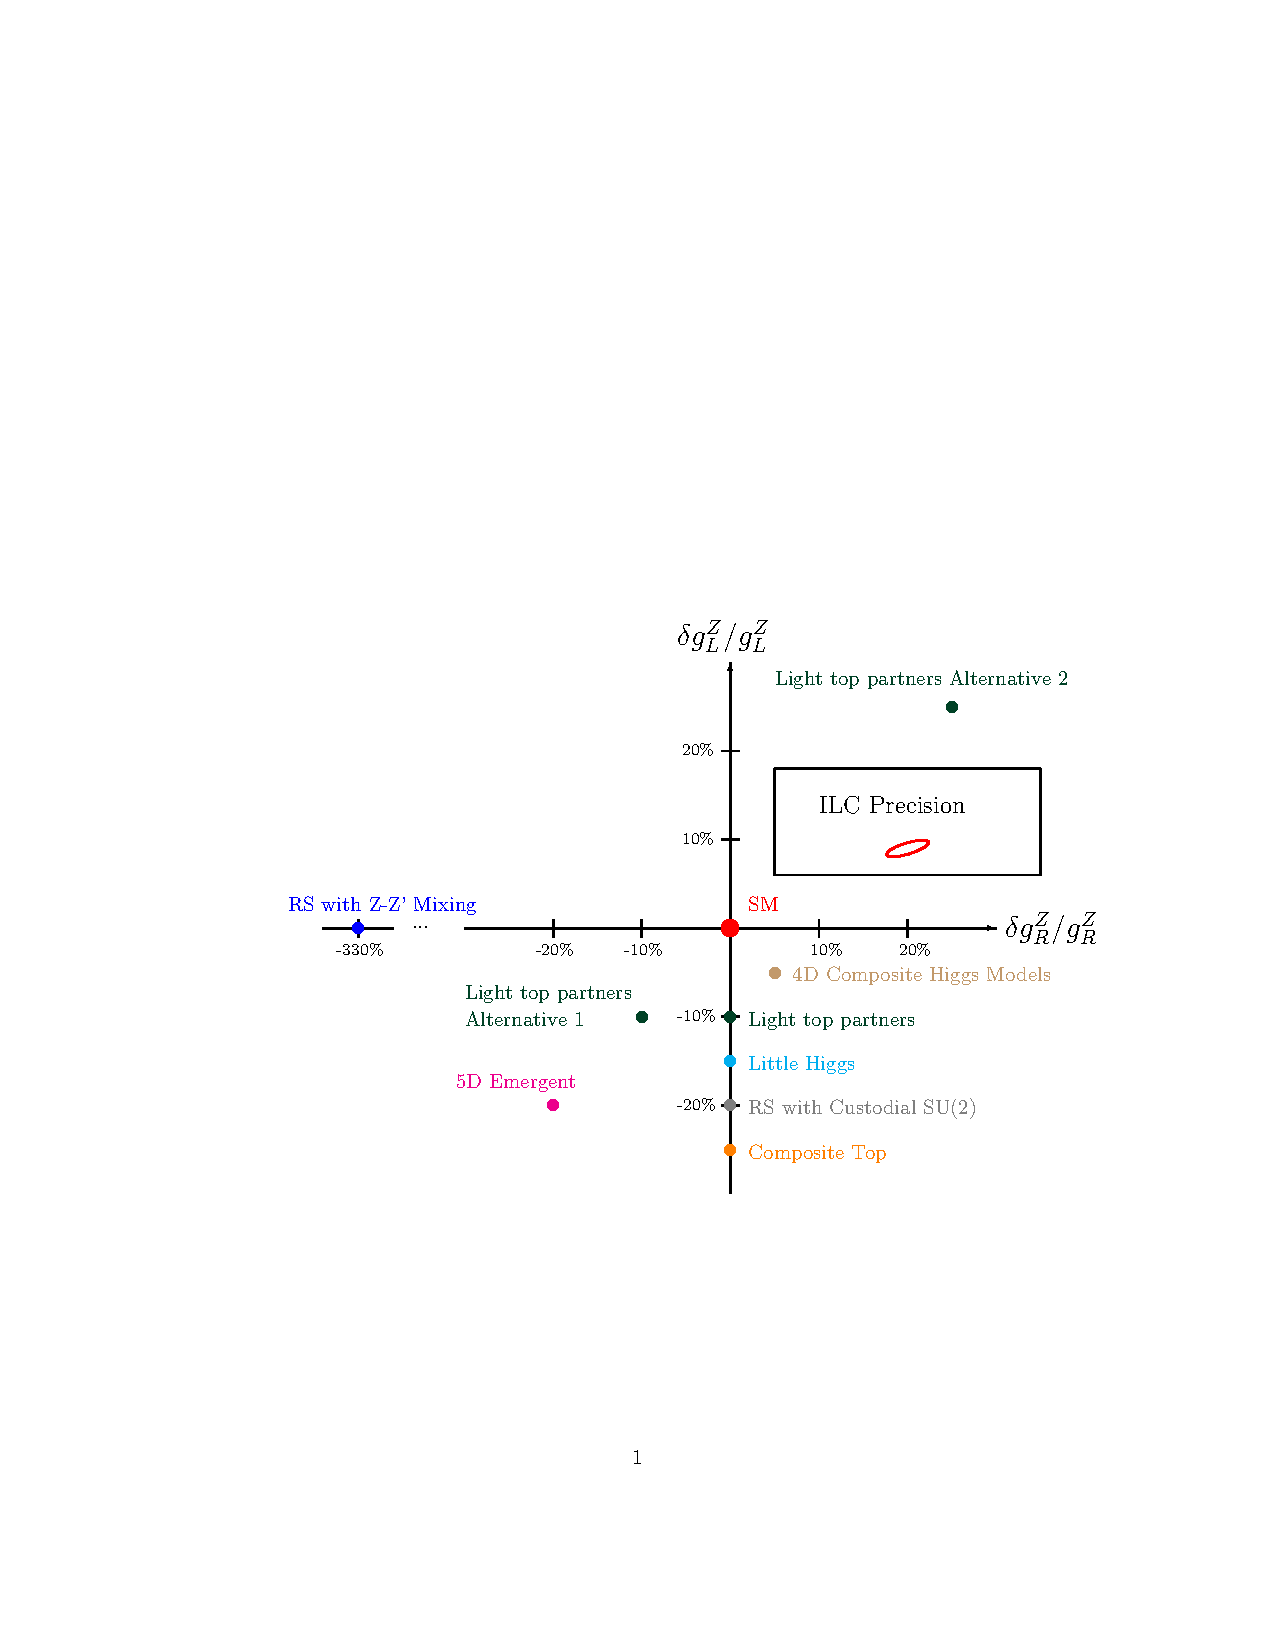
\includegraphics[clip, trim=4cm 7cm 2cm 10cm, width=0.95\textwidth]{ILD/graphics/plot.pdf}
    \caption{\sl Predictions of several models that incorporate Randall-Sundrum (RS) models and/or compositeness or Little Higgs models on the deviations of the left- and right-handed couplings of the $t$~quark to the $Z^0$ boson. The ellipse in the frame in the upper right corner indicates the precision that can be expected for the ILC running at a center-of-mass energy of $\sqrt[]{s} = 500\,GeV$ after having accumulated ${\mathcal L}=500\,fb^{-1}$ of integrated luminosity shared equally between the beam polarizations $P(e^-),\,P(e^+) =\pm0.8,\mp0.3$. The original version of this figure can be found in~\cite{bib:ILCTOP}.}
    \label{fig:DeviationsTop}
  }
\end{figure}
%\begin{figure}[H]
  \centering
\setlength{\unitlength}{1.5mm}
%\setlength{\unitlength}{\textwidth} 

\begin{picture}(150,90)
\linethickness{0.3mm}
%\begin{center}
%compose x axis
  \put(9,33){\line(0,1){2}}
  \put(5,34){\line(1,0){8}}  
  \put(15,34){...} 
  \put(21,34){\vector(1,0){60}} 
  \put(82,33){\Large{$\delta g^Z_R / g^Z_R$}}
  \multiput(31,33)(10,0){5}{\line(0,1){2}} 
  \put(6.5,31){\footnotesize{-330\%}} 
  \put(29,31){\footnotesize{-20\%}} 
  \put(39,31){\footnotesize{-10\%}}
  \put(60,31){\footnotesize{10\%}}
  \put(70,31){\footnotesize{20\%}}
%compose y-axis
  \put(51,4){\vector(0,1){60}} 
  \put(45,66){\Large{$\delta g^Z_L / g^Z_L$}}
  \multiput(50,14)(0,10){5}{\line(1,0){2}} 
  \put(45,13.5){\footnotesize{-20\%}} 
  \put(45,23.5){\footnotesize{-10\%}} 
  \put(45.5,43.5){\footnotesize{10\%}} 
  \put(45.5,53.5){\footnotesize{20\%}}
%Add models
  \put(51,34){\color{red}\circle*{2}} 
  \put(53,36){\color{red}SM}
  \put(51,24){\color{britishracinggreen}\circle*{1.5}}
  \put(53,23){\color{britishracinggreen}Light top partners~\cite{Grojean:2013qca}}
  \put(41,24){\color{britishracinggreen}\circle*{1.5}} 
  \put(21,26){\color{britishracinggreen} Light top partners}
 \put(21,23){\color{britishracinggreen} Alternative 1~\cite{bib:panico-priv}}
  \put(76,59){\color{britishracinggreen}\circle*{1.5}} 
  \put(56,61.5){\color{britishracinggreen} Light top partners Alternative 2~\cite{bib:panico-priv}}
  %\put(53,23){\color{green}Composite Higgs with SO(5)/SO(4)}%~\cite{Grojean:2013qca}}
   \put(51,19){\color{cyan}\circle*{1.5}} 
   \put(53,18){\color{cyan}Little Higgs~\cite{Berger:2005ht}}
  \put(51,14){\color{gray}\circle*{1.5}} 
  \put(53,13){\color{gray}RS with Custodial SU(2)~\cite{Carena:2006bn}}
  \put(51,9){\color{orange}\circle*{1.5}} 
  \put(53,8){\color{orange}Composite Top~\cite{Pomarol:2008bh}}
  \put(31,14){\color{magenta}\circle*{1.5}} 
  \put(20,16){\color{magenta}5D Emergent~\cite{Cui:2010ds}}
  \put(56,29){\color{camel}\circle*{1.5}} 
  \put(58,28){\color{camel}4D Composite Higgs Models~\cite{Barducci:2015aoa}}
  \put(9,34){\color{blue}\circle*{1.5}} 
  \put(1,36){\color{blue}RS with Z-Z' Mixing~\cite{Djouadi:2006rk}}
%make a box to put the ILC precision into
\multiput(56,40)(30,0){2}{\line(0,1){12}} 
\multiput(56,40)(0,12){2}{\line(1,0){30}}
\put(61,47){\large{ILC Precision}}
%embed the covariance ellipse
\color{red}
% Ellipse:  u = 71.0  v = 43.0  a = 2.45336  b = 0.631947  phi = 16.9866 Grad
\qbezier(73.3463, 43.7167)(73.2699, 43.9671)(72.5286, 43.9342)
\qbezier(72.5286, 43.9342)(71.7873, 43.9013)(70.8154, 43.6044)
\qbezier(70.8154, 43.6044)(69.8435, 43.3075)(69.2103, 42.9205)
\qbezier(69.2103, 42.9205)(68.5772, 42.5336)(68.6537, 42.2833)
\qbezier(68.6537, 42.2833)(68.7301, 42.0329)(69.4714, 42.0658)
\qbezier(69.4714, 42.0658)(70.2127, 42.0987)(71.1846, 42.3956)
\qbezier(71.1846, 42.3956)(72.1565, 42.6925)(72.7897, 43.0795)
\qbezier(72.7897, 43.0795)(73.4228, 43.4664)(73.3463, 43.7167)
\end{picture}





\caption{\sl Predictions of several models that incorporate Randall-Sundrum (RS) models and/or compositeness or Little Higgs models on the deviations of the left- and right-handed couplings of the $t$~quark to the $Z^0$ boson. The ellipse in the frame in the upper right corner indicates the precision that can be expected for the ILC running at a centre-of-mass energy of $\sqrt[]{s} = 500\,GeV$ after having accumulated ${\mathcal L}=500\,fb^{-1}$ of integrated luminosity shared equally between the beam polarisations $P(e^-),\,P(e^+) =\pm0.8,\mp0.3$. The original version of this figure can be found in~\cite{bib:ILCTOP}.}
\label{fig:models-rp}
\end{figure}
%Supersymmetric models  -  have different set of Higgs couplings to the up and down type quarks.
\subsection{Status of the measurements and simulation studies}
%mass measurements
\subsubsection{LHC and TeVatron measurements}
The initial state at hadron colliders allows a strong production of the top quark pairs via $gg\to t\bar{t}$ or $q\bar{q}\to t\bar{t}$ processes. 
Therefore, the hadron machines can measure the top mass and strong couplings of the top quark with a high precision. 
The TeVatron, which has proton-antiproton beams, can produce single top process at a higher rate than proton-proton machines. 
This process involve $tbW$ vertex and therefore, its cross section depends on weak coupling of the top quark. 
The measurement of single top cross section at TeVatron is found to be consistent with the \sm\ predictions~\cite{bib:TeVstop} with about 16\% uncertainty.

The forward-backward asymmetry at hadron colliders for strong interaction vertex $gt\bar{t}$ has been measured to be consistent with the \sm\ expectations~\cite{bib:TeVAfb}. 

To measure the electroweak couplings of the top quark at hadron colliders, the associate production of top quark pair with $Z^0$ boson is required. 
Study of $t\bar{t}Z^0$ process has been done at LHC experiments using Run I data with $\sqrt{s} = 8$\,TeV shows compatible rates of the signal process with the \sm, but more statistics is required to measure the cross section precisely~\cite{bib:CMSttz2014}. 
Including the Run II data of the LHC with a higher center-of-mass energy will significantly improve $t\bar{t}Z^0$ measurement.
%Main channel of the top quark production is gluons

%ttZ cross section measurements

\subsubsection{Measurements at LEP and SLC}
The electron-positron colliders have a large production cross section of $e^+e^- \to q\bar{q}$ process mediated by $Z^0$ boson or a virtual photon. The total cross sections of various \sm\ processes for $e^+e^-$ machines are shown in Fig.~\ref{fig:LCcrosssection}.

The circular LEP~I and the linear SLC colliders staged at $Z^0$ pole, where the $q\bar{q}$ cross section is maximal, benefiting from significantly increased event rate. 
The measurements resulted in an extremely precise cross section determination and a forward-backward asymmetry measurements. 
The measured cross section value has full compatibility with the \sm\ calculations. 
On the other hand, the measured b-quark forward-backward asymmetry $A_{FB}^b$ value has  2.5\,$\sigma$ tension with a recent electroweak fit predictions~\cite{bib:AfbSMFit}.

The measurements outside $Z^0$ pole were done by the LEP~II collider, which collected the most integrated luminosity at around 190\,GeV energy, where $e^+e^- \to W^+W^-$ process has a maximum of its cross section.
The measured $A_{FB}^b$ at this center-of-mass energy is within 2\,$\sigma$ from tree level \sm\ prediction.

%$A_{fb}^b(\sqrt[]{s} = 190.7\,\text{GeV})=0.51\pm0.058$
Unfortunately, the beam energies of LEP~II and SLC was not high enough to produce single top or top quark pairs, therefore, the precise determination of the top electroweak couplings is left for the future electron-positron machines.

%2.5s tension by LEP in bbar asymmetry
\subsubsection{Future linear colliders}

The available today acceleration technologies allow construction and running of a linear electron-positron collider at center-of-mass energies higher than top pair production threshold. The precision of the linear colliders allows detection and reconstruction of all \sm\ decay modes of the top quark: fully leptonic, semileptonic and fully hadronic decays. 

As can be seen from expression of the forward-backward asymmetry~(\ref{formula:AfbForm_3}), the sensitivity to axial form factors is proportional to the fermion velocity $\beta$, therefore, the higher beam energies, like 500\,GeV stage at the ILC are preferred for study of electroweak top quark couplings. 
The b-quark coupling analysis can be done at all center-of-mass energies, scheduled at the ILC project.
\begin{figure}[h]
{\centering
    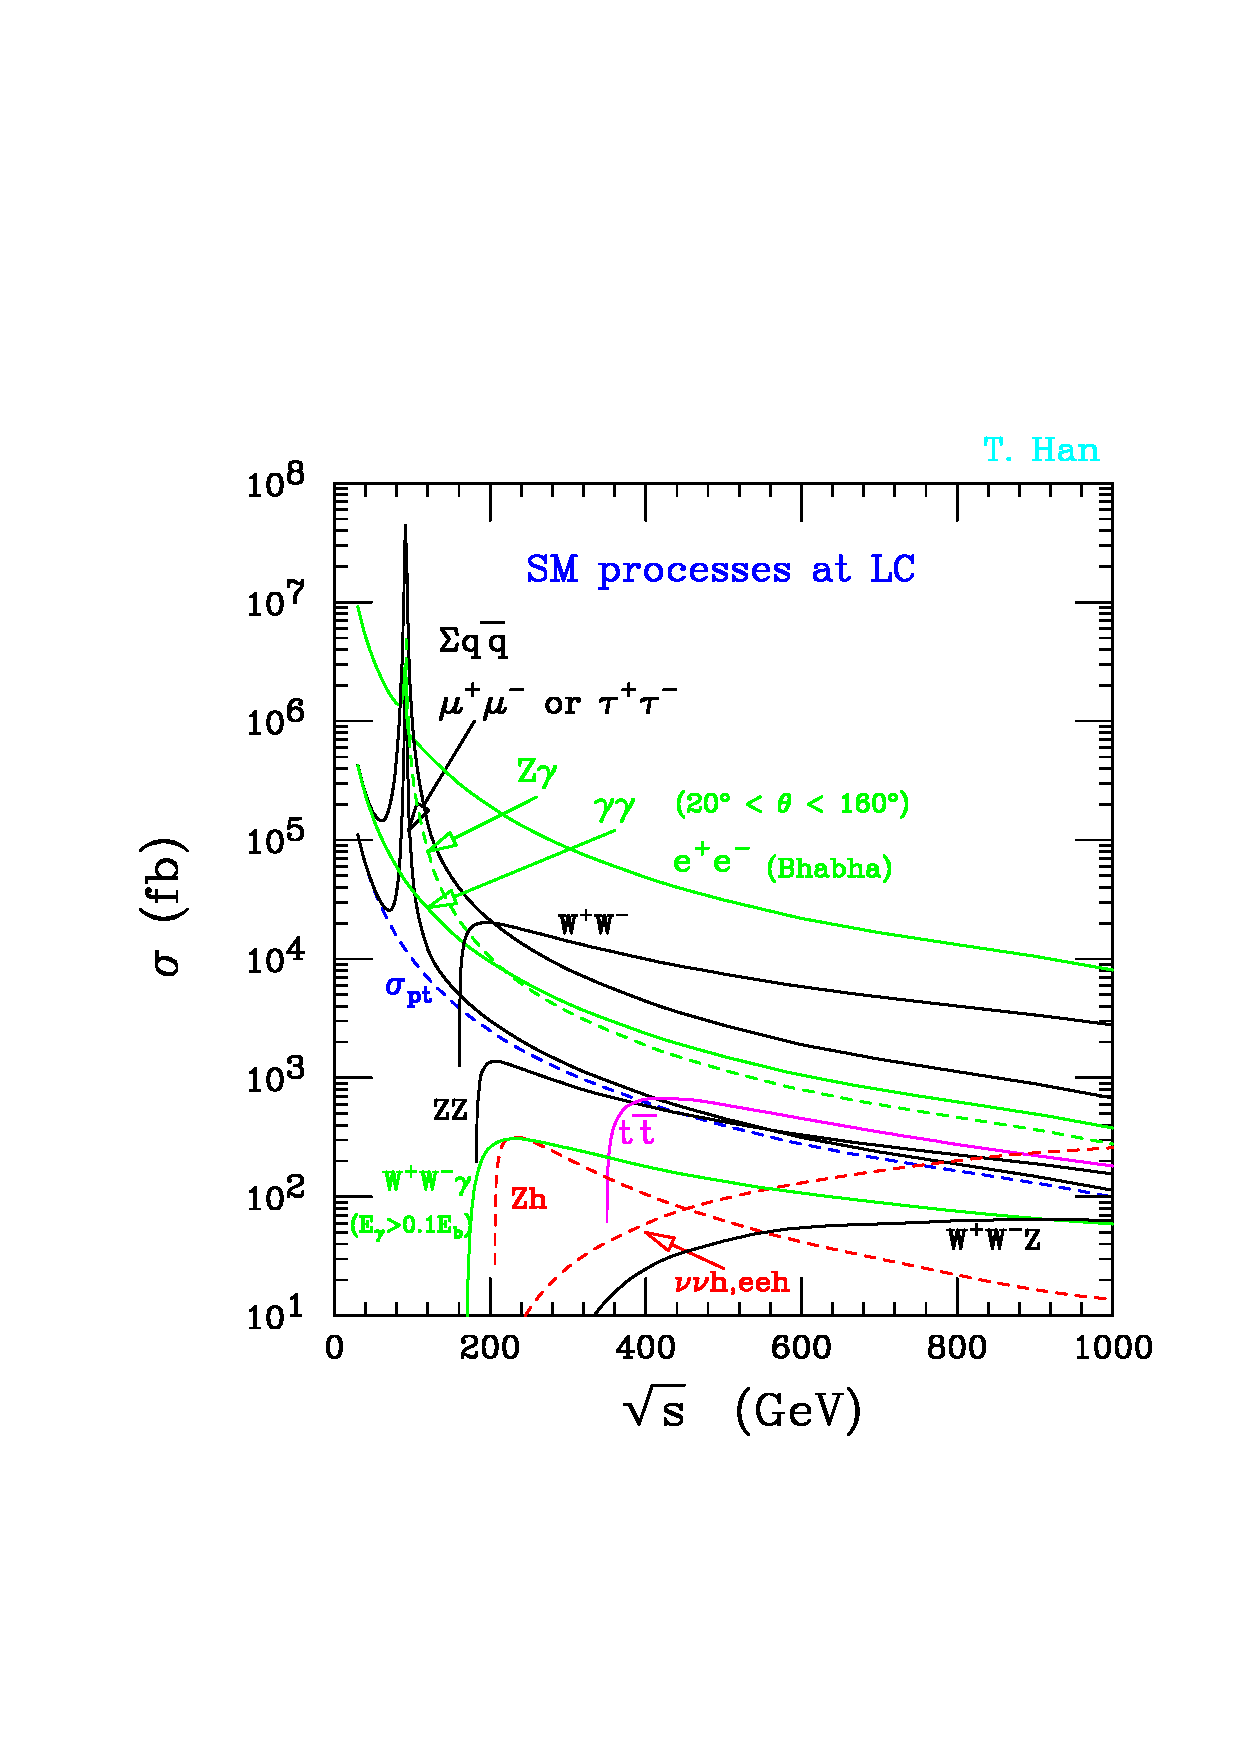
\includegraphics[clip, trim=0.5cm 5cm 0.5cm 7cm, width=0.95\textwidth]{ILD/graphics/epem_sm-hepph.pdf}
    \caption{\sl Tree-level cross sections of major \sm\ processes at linear colliders as function of center-of-mass energy assuming no polarization of the initial state.}
    \label{fig:LCcrosssection}
  }
\end{figure}


%Matrix element method fully leptonic
Such assets of the future $e^+e^-$ colliders as high signal-to-noise ratio and high-granularity of the detectors allow to use Matrix Element Method to compute the form factors from a kinematical fit of the top pair decay products. 
This method can be applied at the ILC for fully leptonic decay of the top quark pair. 
%CLIC
The study of the top couplings at CLIC was done in [Garcia Garcia thesis]. 

The first top quark electroweak coupling analysis at the ILC was carried out by the ILC group in Orsay, resulting in the paper~\cite{bib:ILCTOP}, where the uncertainties on the form factors \ref{formula:SMformFactors_3} and the couplings \ref{formula:EWcouplings_3} were estimated using the ILD environment.


The first challenge of the $A_{FB}$ measurements in hadronic channels is the quark charge identification. Therefore, the semileptonic top decays are used in~\cite{bib:ILCTOP}, where lepton from leptonic top quark decay provides the charge information, and jets from hadronic top quark decays are used for top polar angle reconstruction. 
The next challenge is the assigning the lepton to the bottom quark jet from the same parent top quark, which is not trivial in left-handed case because of the lepton migration effect, caused by $W^\pm$ kinematics. There was found two possible ways to solve the lepton migration effect problem - the kinematical $\chi^2_{top}$ cut or finding the correct combination with the b-jet charge. The advantage of the combination with the b-jet charge is that this method do not require precise knowledge of the top quark decay kinematics, as it is needed for the $\chi^2_{top}$ cut method. The reconstructed top polar angle distribution for semileptonic decay of the top quark pair is shown in Fig.~\ref{fig:ILCTOPAFB}.
The first attempt to use the jet charge technique in fully hadronic top decays was done by [Amjad thesis], but it required large simulation-dependent corrections. 


\begin{figure}[H]
	\centering
	\begin{subfigure}{0.5\textwidth}
		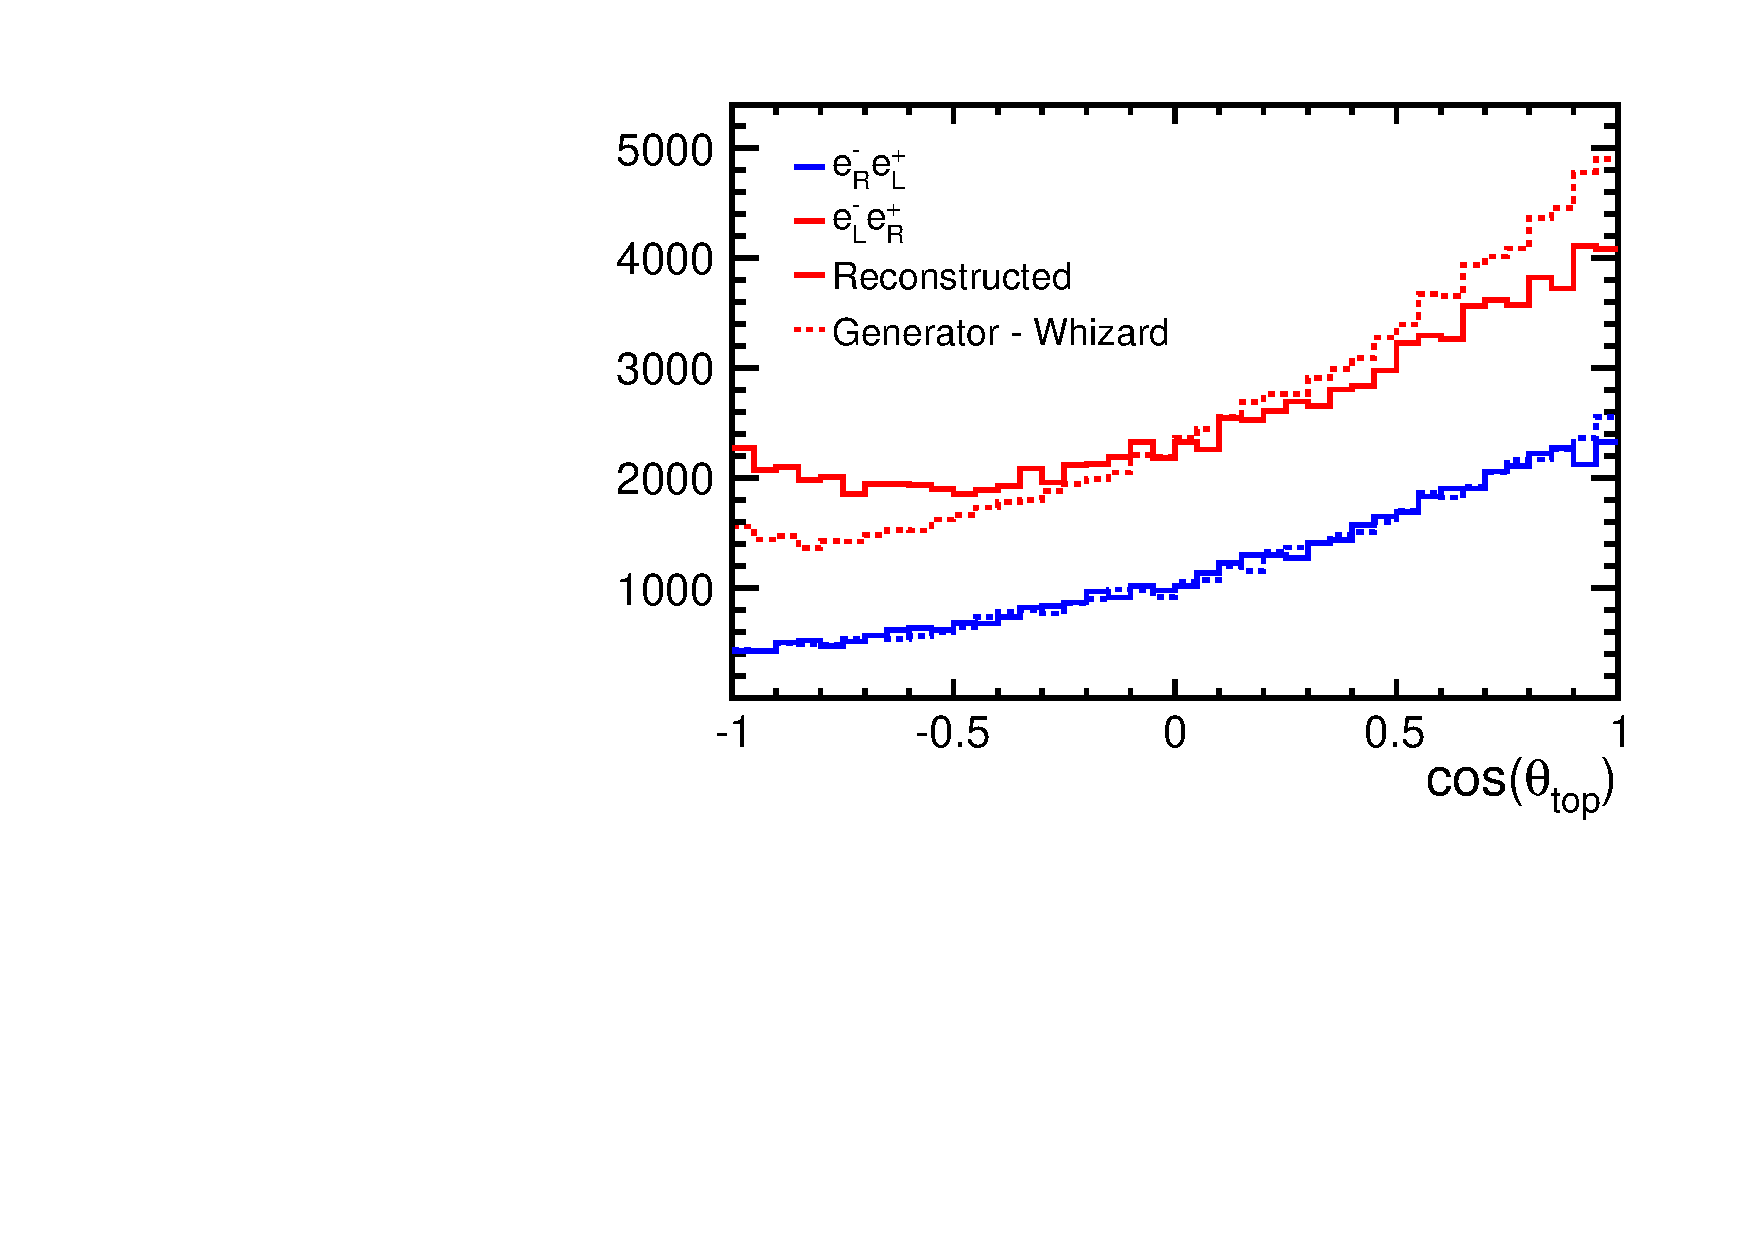
\includegraphics[width=0.95\textwidth]{ILD/graphics/EPS_AFB_nocut.pdf}
		\caption{\label{fig:ILCTOPAFB_a_3} }
	\end{subfigure}% 
	\begin{subfigure}{0.5\textwidth}
		\centering
		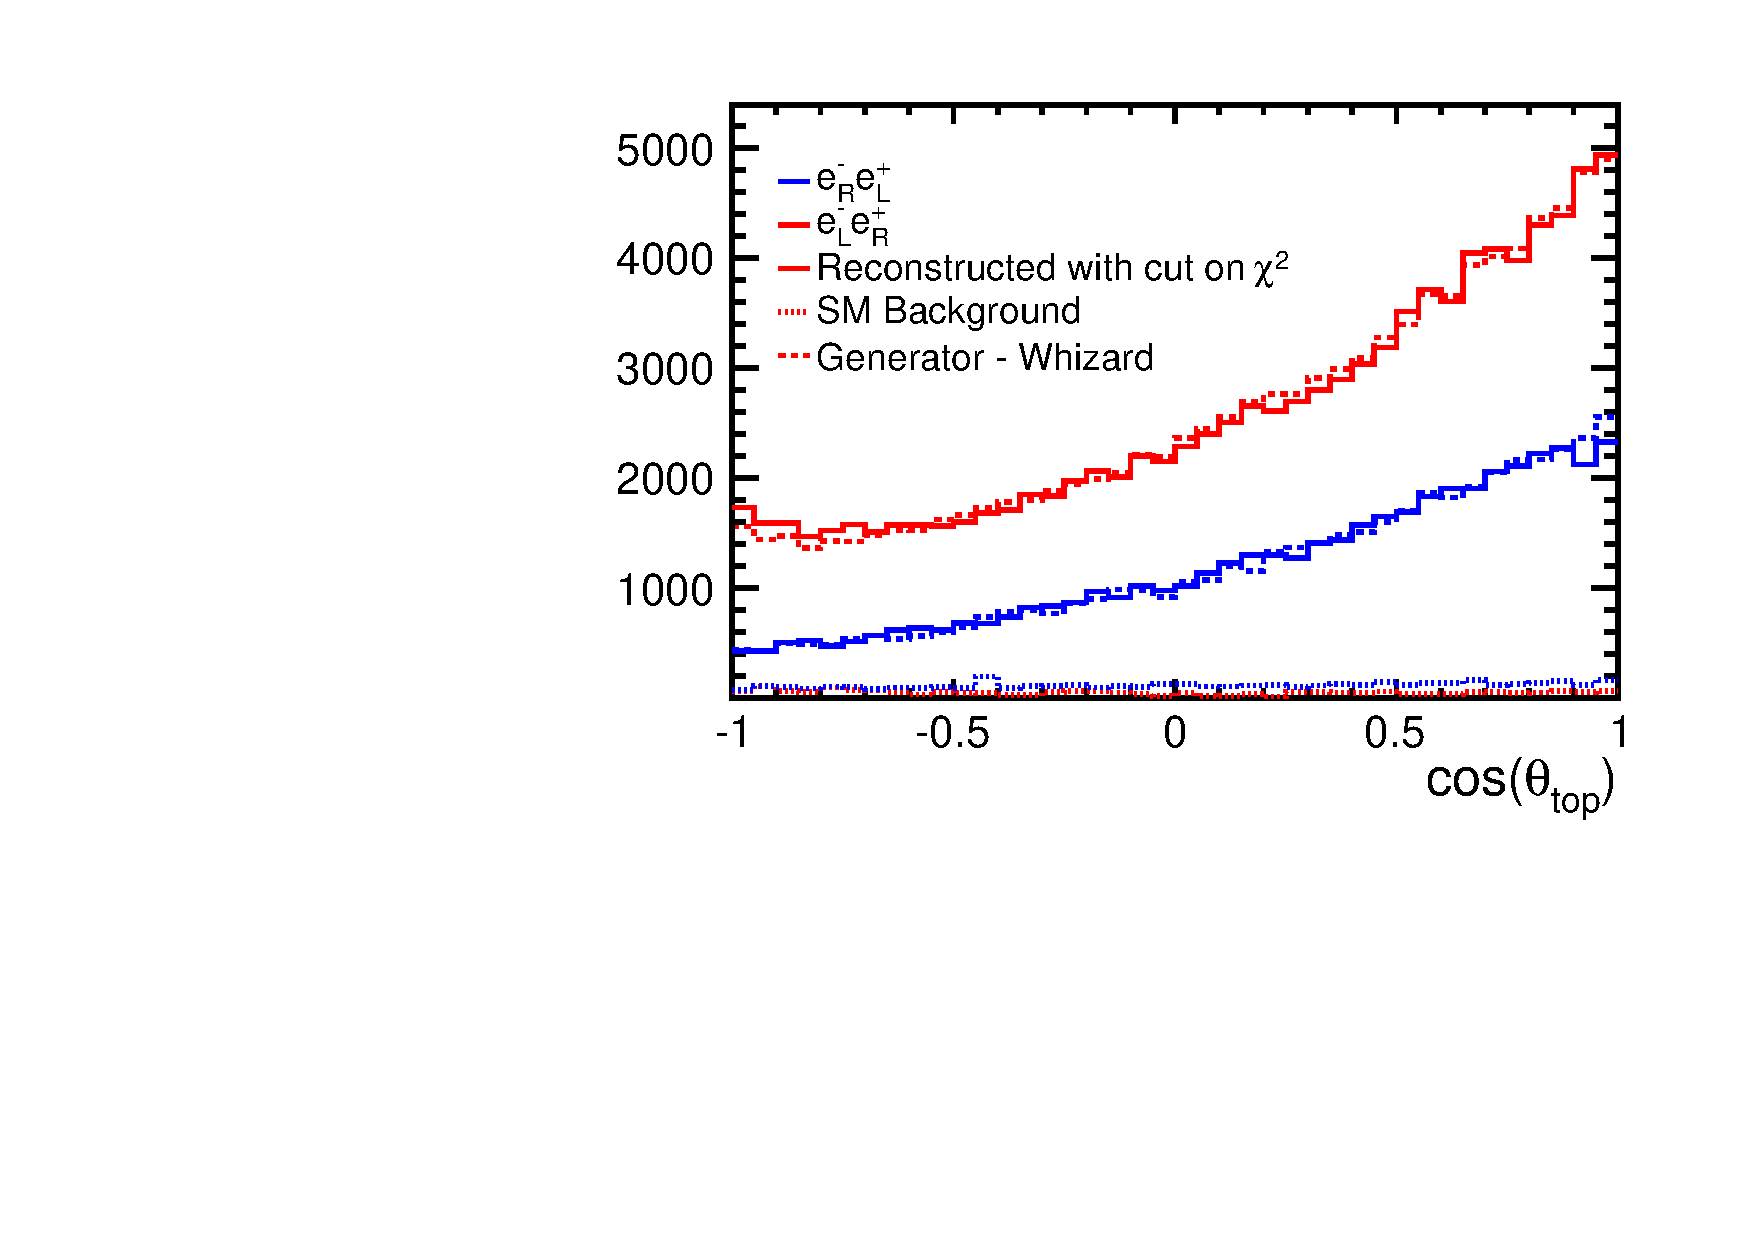
\includegraphics[width=0.95\textwidth]{ILD/graphics/AFB_wbkg_chi2cut.pdf}
		\caption{\label{fig:ILCTOPAFB_b_3} }
	\end{subfigure}
	\caption{\sl Reconstructed top quark polar angle before (a) and after $\chi^2_{top}$ cut (b) distributions compared with the prediction by the event generator for two configurations of the beam polarizations~\cite{bib:ILCTOP}. }

	    \label{fig:ILCTOPAFB}
\end{figure}

The development of the jet charge measurement will open access to the fully hadronic top decay channels without any Monte-Carlo corrections and, moreover, it will allow a study of electroweak coupling of the bottom quark, which was never done using ILC environment. 


%Study of precision of ILC on top couplings were made by Amjad et al. using semileptonic decays. 
%Central problem: migration effect of the lepton from W. 
%B charge was first used as a way to remove migration effect by Jeremy for semileptonic channel.  and Amjad for hadronic one. 
%Development of jet charge measurement technique willl increase the statistics for semileptonic channel, and open hadronic top decays. 
%The jet charge measurement is the only way to study the bbbar process.  

%%%%%%%%%%%%%%%%%%%%%%%%%%%%%%%%%%%%%%%%%%%%%%%%
%%%%%%%%%%%%%%%%%%%%%%%%%%%%%%%%%%%%%%%%%%%%%%%%
%%%%%%%%%%%%%%%%%%%%%%%%%%%%%%%%%%%%%%%%%%%%%%%%

\section{Jet charge reconstruction}
\label{sec:JetChargeReconstruction}
An information about a bottom jet charge is useful for all \sm\ processes, where b-jets appear as decay products, particularly, it can be applied for reconstruction of forward-backward asymmetry in $e^+e^-\to t\bar{t}$ and $e^+e^- \to b\bar{b}$ processes. 
The main challenge for these processes is a high purity and efficiency of the charge reconstruction, which requires an ultimate performance from all subdetectors of the experiment. 

One of the main goals of this thesis is to increase purity and efficiency of the b-jet charge measurement using ILD environment. 
To do so, first, it is necessary to measure performance of the standard reconstruction algorithm and find sources of charge impurities, and then develop an algorithm to improve it. 



\subsection{Setup of the study}

All studies in this and next chapters are done using full simulation of the baseline ILD experiment. 
The jet charge measurement study uses $e^+e^- \to b\bar{b}$ at $\sqrt[]{s} = 250$\,GeV and semileptonic decay mode of the $e^+e^- \to t\bar{t}$ at $\sqrt[]{s} = 500$\,GeV processes generated using {\sc whizard}~1.95 event generator. 
The hadronization of the quarks and gluons is done by the {\sc pythia}~6.205 event generator. 
The ILD layout and the interaction of particles with the detector material are simulated by the {\sc mokka} framework, largely based on the \geant\ toolkit, which is also responsible for creation of the hits in the simulated subdetectors. 

All reconstruction algorithms, along with the {\sc mokka} framework are part of the {\sc ilcsoft} software toolkit.
The modular structure of the {\sc ilcsoft} allows to  launch each reconstruction algorithm independently. 

The ILD collaboration defines the order of the standard reconstruction chain, which is applied to all studies done using the full simulation of the ILD experiment. 

The most relevant standard reconstruction algorithms of the {\sc ilcsoft} for the jet charge measurement are:
\begin{itemize}
\item The MarlinTrk package organize the hits, created by particles in the ILD trackers into reconstructed tracks. The track parametrization in described in~\cite{bib:LCIOtrack}. Each reconstructed track has an associated covariance matrix;
\item The PandoraPFA package is responsible for the clusterization of the calorimeter hits and creation of the Particle Flow Objects. The track covariance matrix is used to compute the covariance matrix of the reconstructed particle momentum; 
\item The primary and secondary vertex reconstruction is done by the LCFI+ algorithm. 
\end{itemize}
The jet clustering algorithms can be configured and launched according to the analysis requirements. 
The flavor-tagging at the ILD experiment will serve to separate out jets from bottom and charm quarks from the light quark or gluon jets.
The flavor-tagging algorithm within the LCFI+ package provides b- and c-probability information of a reconstructed jet, called b- and c-tagging, respectively.

%\subsubsection{Simulated samples}

%\subsubsection{ILC reconstruction software}
%\subsubsection{Vertex detection algorithms}

\subsection{Bottom quark topology}
%The key parameter for the b-jet charge reconstruction is the initial b-quark energy, which are within a similar range for 250\,GeV $b\bar{b}$ pair and 500\,GeV $t\bar{t}$ pair production processes.   %The key particle is the b-quark 
%The b-jet charge measurement is based on 
The only way to measure the initial b-quark charge in a b-jet is to measure the charge of the corresponding b-hadron. 
Therefore, one needs to know precisely the properties of the underlying hadrons. 


The b-quark hadronization modes are displayed in Table~\ref{table:bhadrons}.
        \begin{table}[H]
        \begin{center}
        \begin{tabular}{l c c }
        \hline
        			& Branching ratio & $c\tau$ \\
        \hline
            \Bm\ meson & $40.4 \pm 0.6 $\% & 450\,$\mu$m \\
            \Bz\ meson & $40.4 \pm 0.6 $\% & 455.4\,$\mu$m  \\

            \Bzs\ meson & $10.3 \pm 0.5 $\% & 453.3\,$\mu$m   \\
         \hline
            b-baryon & $8.9 \pm 1.3 $\% & $\approx$ 447\,$\mu$m  \\

        \hline
        \end{tabular}
        \end{center}
        \caption{\sl Hadronization modes of the b-quark~\cite{bib:PDG}. }
        \label{table:bhadrons}
        \end{table}

These branching fractions are approximate and may have a dependency on the initial and final state kinematic and production environment~\cite{bib:PDG}.
However, the presence of the \Bzs\ meson increase number of the neutral hadronization modes, which will cause additional complications for the charge measurement. 

%b-hadron decays, typically, the charged pions, kaons, leptons or protons, 
Due to the Lorentz boost given by the initial b-quark energy, the b-hadron can travel several millimeters before its decay. Due to this flight distance, the charged particles from the b-hadron decays will have an offset with respect to the primary interaction point, which is the main signature of the b-quark jets. 

%Therefore we expect two vertices
The B meson have very frequent $D^0$ or $D^\pm$ meson decay modes, mediated by the weak interaction. The charmed $D$ mesons have $c\tau \approx 120 - 300$\,$\mu$m, which gives a possibility to the charmed mesons to travel away from the initial B meson decay vertex. 
Hence, one expects to detect two vertices from one b-jet in most of the cases: the secondary, which corresponds to the b-hadron decay, and the tertiary vertex created by the c-hadron decays. 

The $D^0$ or $D^\pm$ mesons have approximately 74\% probability to decay into a charged $K^\pm$ meson plus other particles. The $K^\pm$ mesons have a long lifetime with $c\tau = 3.7$\,m and a high mass of 493.6\,MeV comparing to another charged particles from B meson decays, like pions or leptons, which can be use to identify kaons by the energy deposition. The $K^\pm$ mesons from B meson decays are the end products of the $b\to c\to s$ decay chain mediated by the weak interaction, therefore, the charge of the $K^\pm$ mesons should correlate with the initial b-quark charge. 
On contrary, the b-baryons tend to produce protons, which have an opposite sign of charge to the initial b-quark charge. 

%%%%%%%%%%%%%%%%%%%%%%%%%%%%%%%%%%%%%%%%%%%%%%%%%%%%%%%
%%%%%%%%%%%%%%%%%%%%%%%%%%%%%%%%%%%%%%%%%%%%%%%%%%%%%%%
%%%%%%%%%%%%%%%%%%%%%%%%%%%%%%%%%%%%%%%%%%%%%%%%%%%%%%%
\subsubsection{Generated vertices}
A typical output of the event generators is a list of generated particles with parent-child relations.The TruthVertexFinder algorithm was developed to find the generated vertices, and included into the {\sc ilcsoft} distribution. This algorithm detects the generated b-hadrons, finds the related charged particles, which can leave reconstructable tracks and organizes them into the generated secondary or tertiary vertices.


\begin{figure}[h]
{\centering
    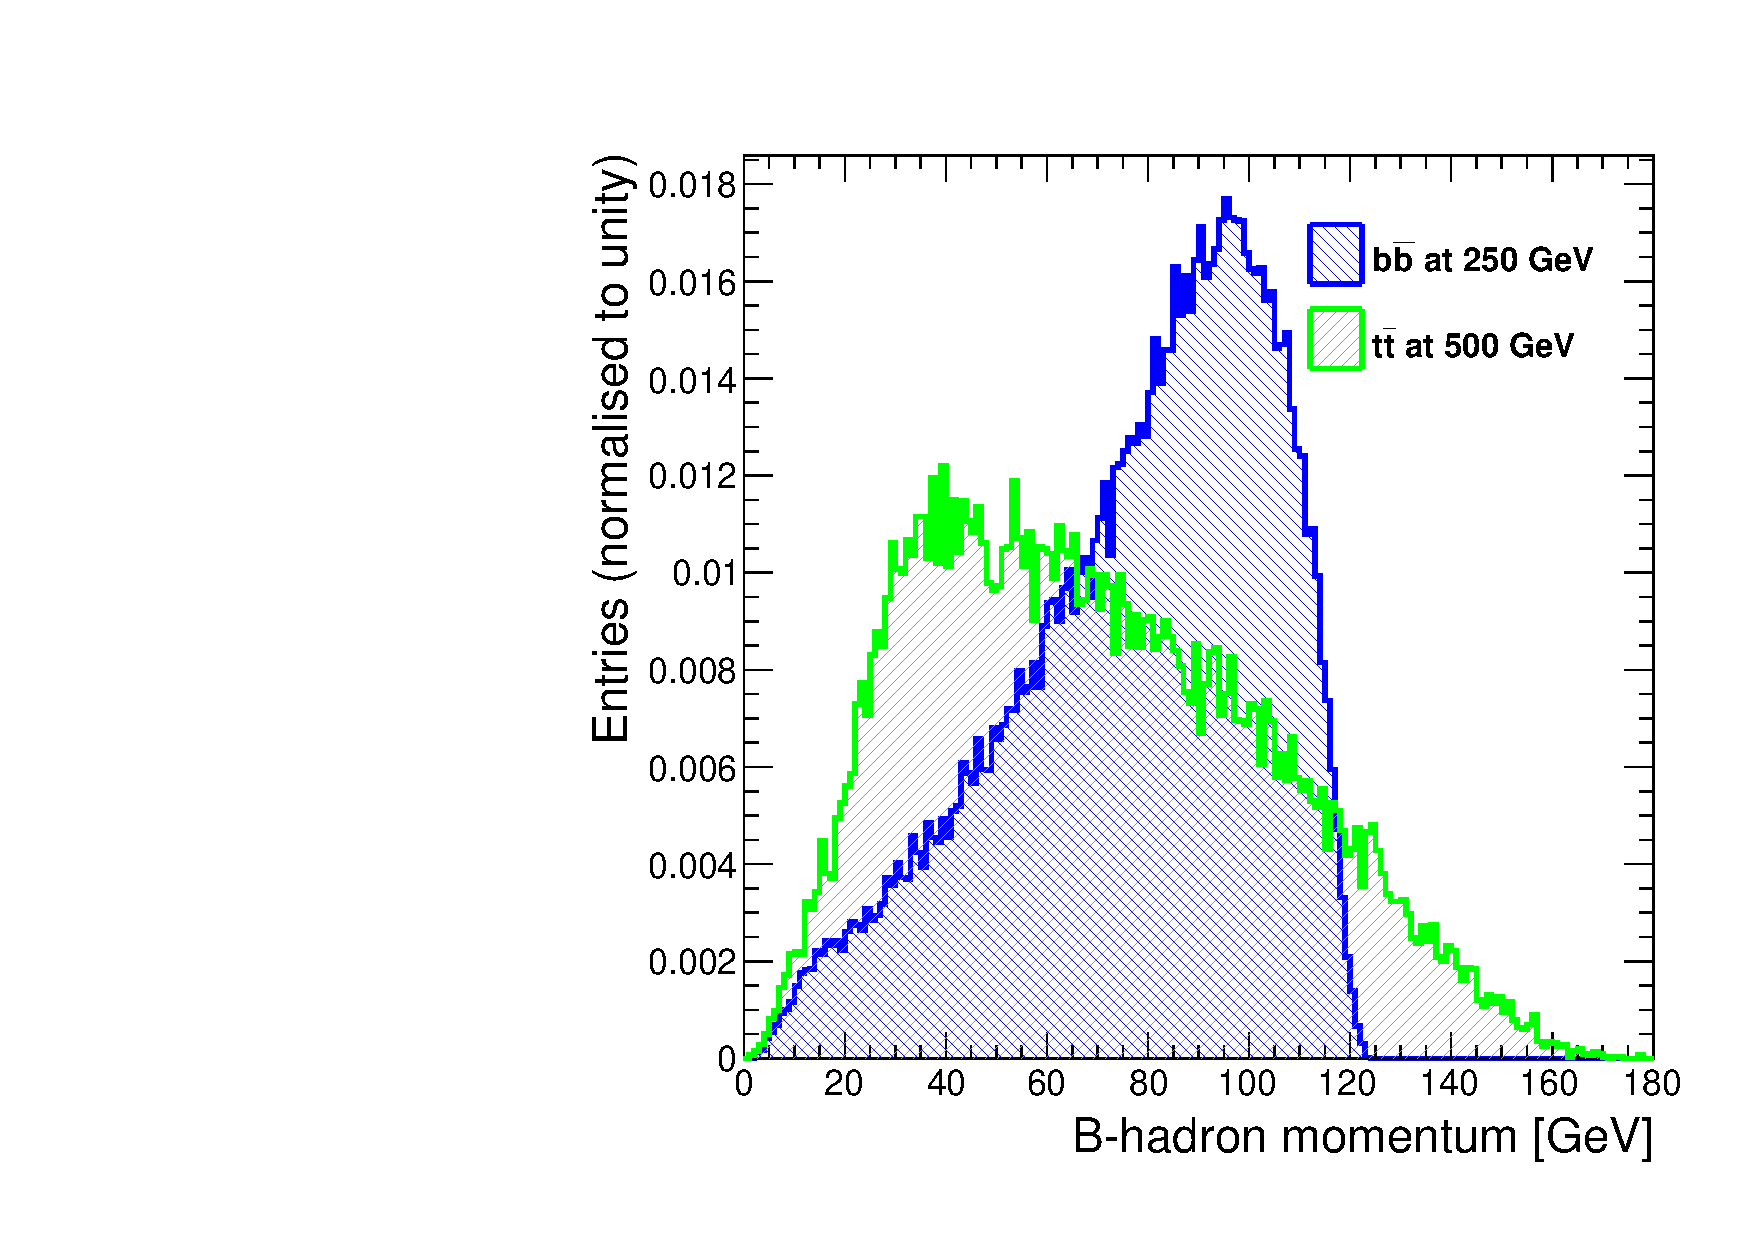
\includegraphics[width=0.45\textwidth]{ILD/plots/gen-hadron-momentum.pdf}
    \caption{\sl Generated b-hadron momentum by {\sc pythia} for two signal processes.}
    \label{fig:GenHadronMomentum_3}
  }
\end{figure}
%Generator distributions
The distributions of the b-hadron momentum, generated by {\sc pythia} for the 250\,GeV $b\bar{b}$ and the 500\,GeV $t\bar{t}$ pairs are within the same energy range as it is shown in Fig.~\ref{fig:GenHadronMomentum_3}.

%The b-hadrons can be identified by measuring the charged tracks, which have an offset from primary interaction point caused by the b-hadron lifetime.
%B*
The high-energy b-quarks can hadronize into excited states of the b-hadrons, which can decay into a ground state by emitting charged or neutral pion. 
The charged pion from the excited b-hadrons can distort the charge multiplicity distributions and further comparison with the reconstructed vertices, therefore, the TruthVertexFinder selects only ground state hadrons within a decay chain. 

The TruthVertexFinder is able to find vertices from b-hadron decays and subsequent c-hadron decay vertices. The distributions of generated b- and c-vertices are displayed in Fig.~\ref{fig:GenVtx_3}. The c-vertex multiplicity distribution is consistent with~\cite{bib:PDG}. One can notice that about 31\% of the b-vertices and 13\% of the c-vertices decay into one generated prong, which poses a challenge to the vertexing algorithms. 

\begin{figure}[H]
\centering
\begin{subfigure}{0.5\textwidth}
    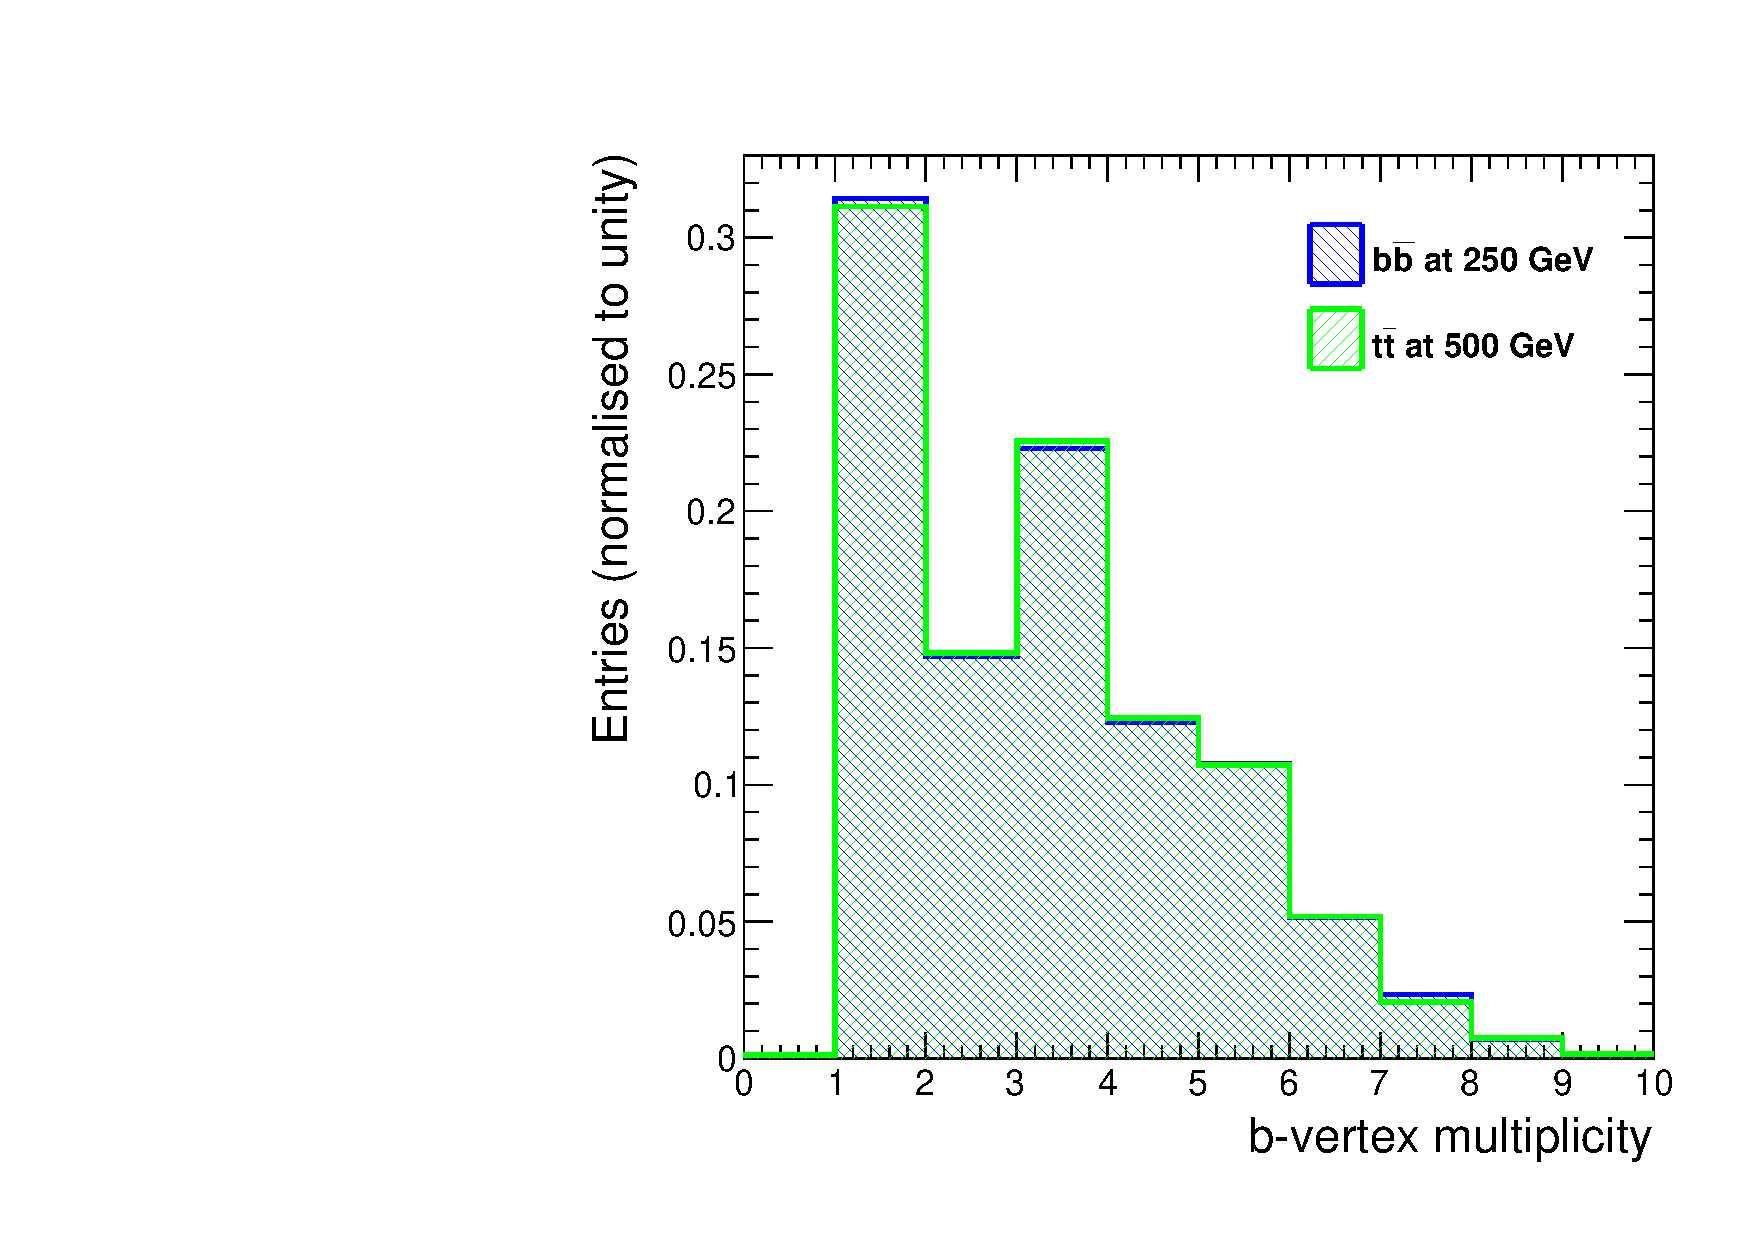
\includegraphics[width=0.95\textwidth]{ILD/plots/gen-b-vtx.pdf}
\caption{\label{fig:GenVtx_a_3} }
\end{subfigure}% 
  \begin{subfigure}{0.5\textwidth}
\centering
    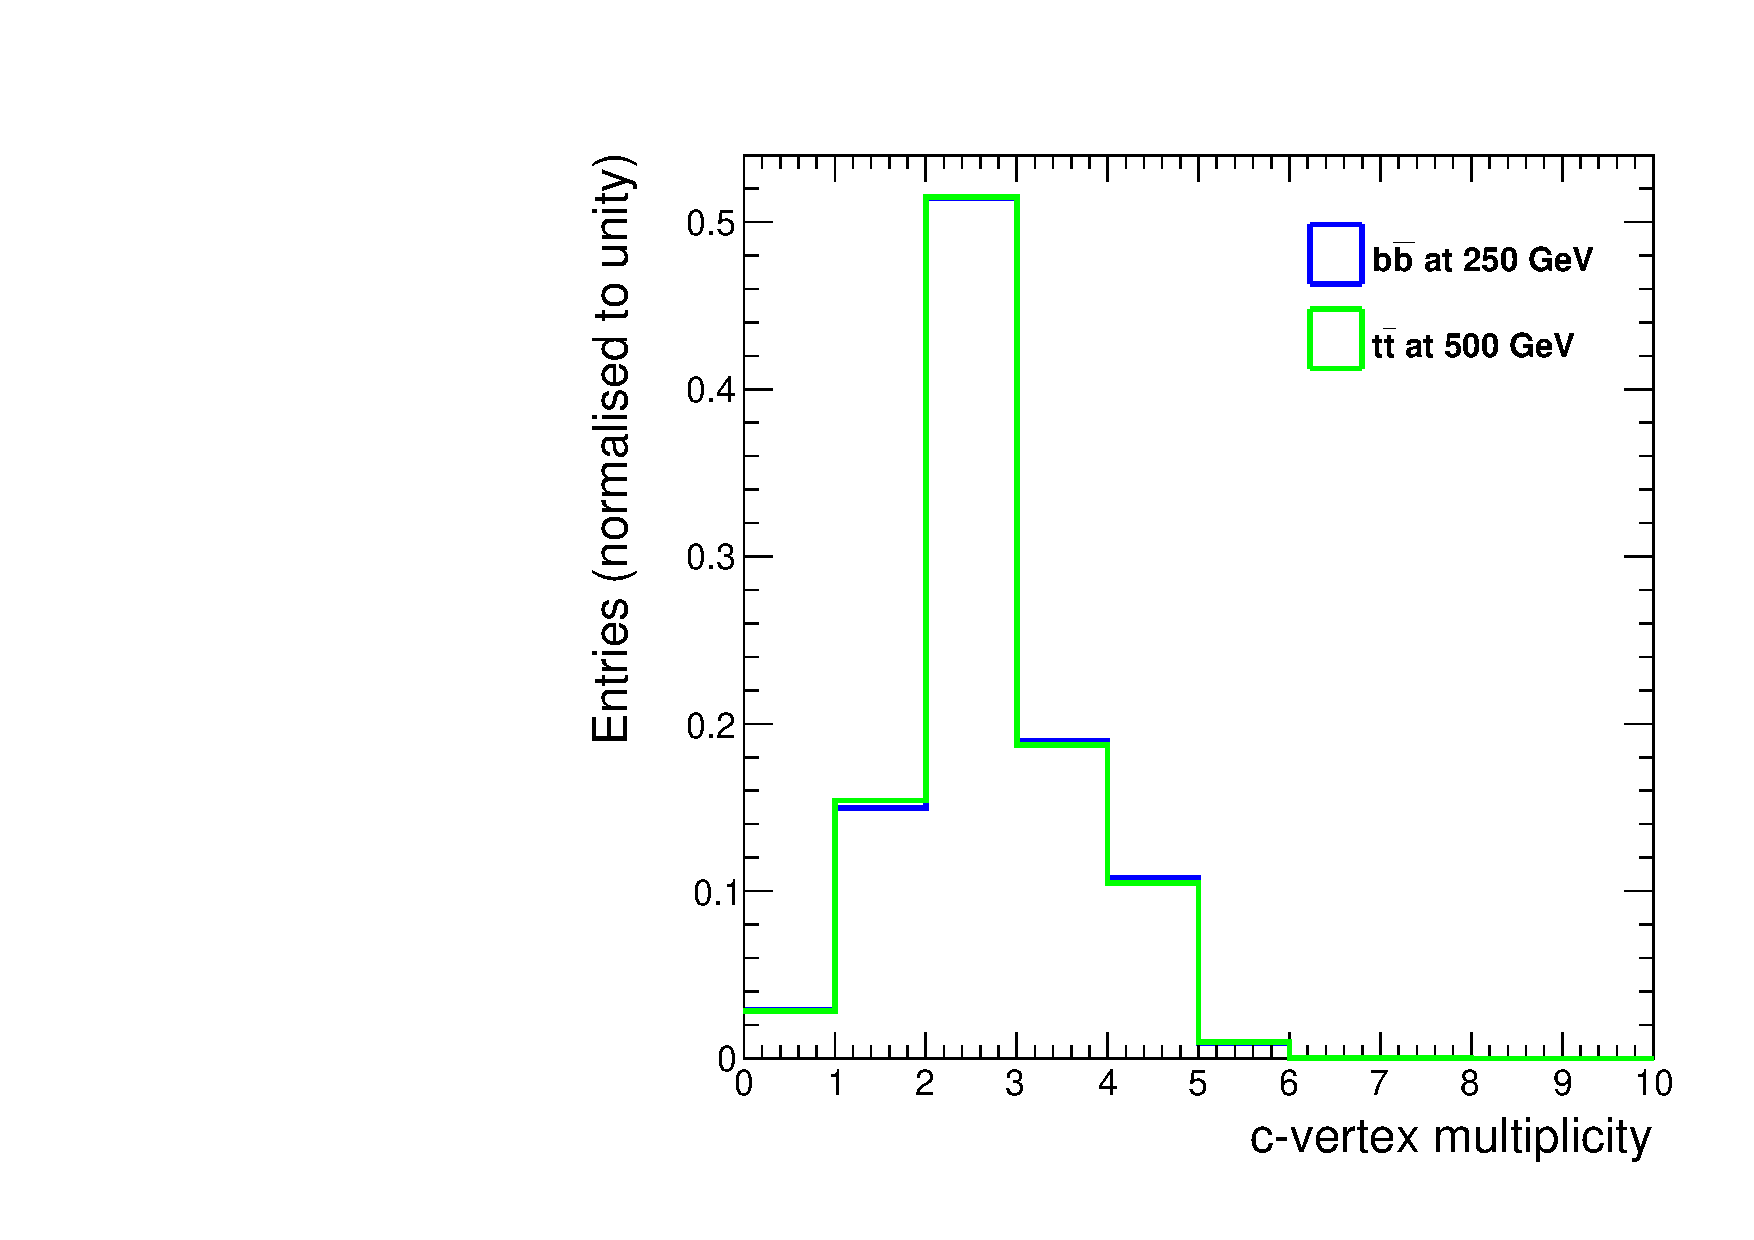
\includegraphics[width=0.95\textwidth]{ILD/plots/gen-c-vtx.pdf}
\caption{\label{fig:GenVtx_b_3} }
\end{subfigure}
    \caption{\sl Distributions of the b-vertex charge multiplicity~(a) and c-vertex charge multiplicity~(b). }
    \label{fig:GenVtx_3}
\end{figure}

The particle offset or the impact parameter is a minimal distance between the particle trajectory and the interaction point. 
This is the main observable used by the vertex reconstruction algorithms. 
The offset distributions of the generated b-vertex and c-vertex prongs are shown in Fig.~\ref{fig:GenVtxOffset_3}.
Majority of the generated prongs have large offsets above the ILD impact parameter resolution of 5\,$\mu$m. 
As can be seen from Fig.~\ref{fig:GenVtxOffset_3}, the c-vertex prong offsets are larger than b-vertex prong offsets, because of the additional distance traveled by c-hadron from the b-hadron decay point. 

\begin{figure}[h]
\centering
\begin{subfigure}{0.5\textwidth}
    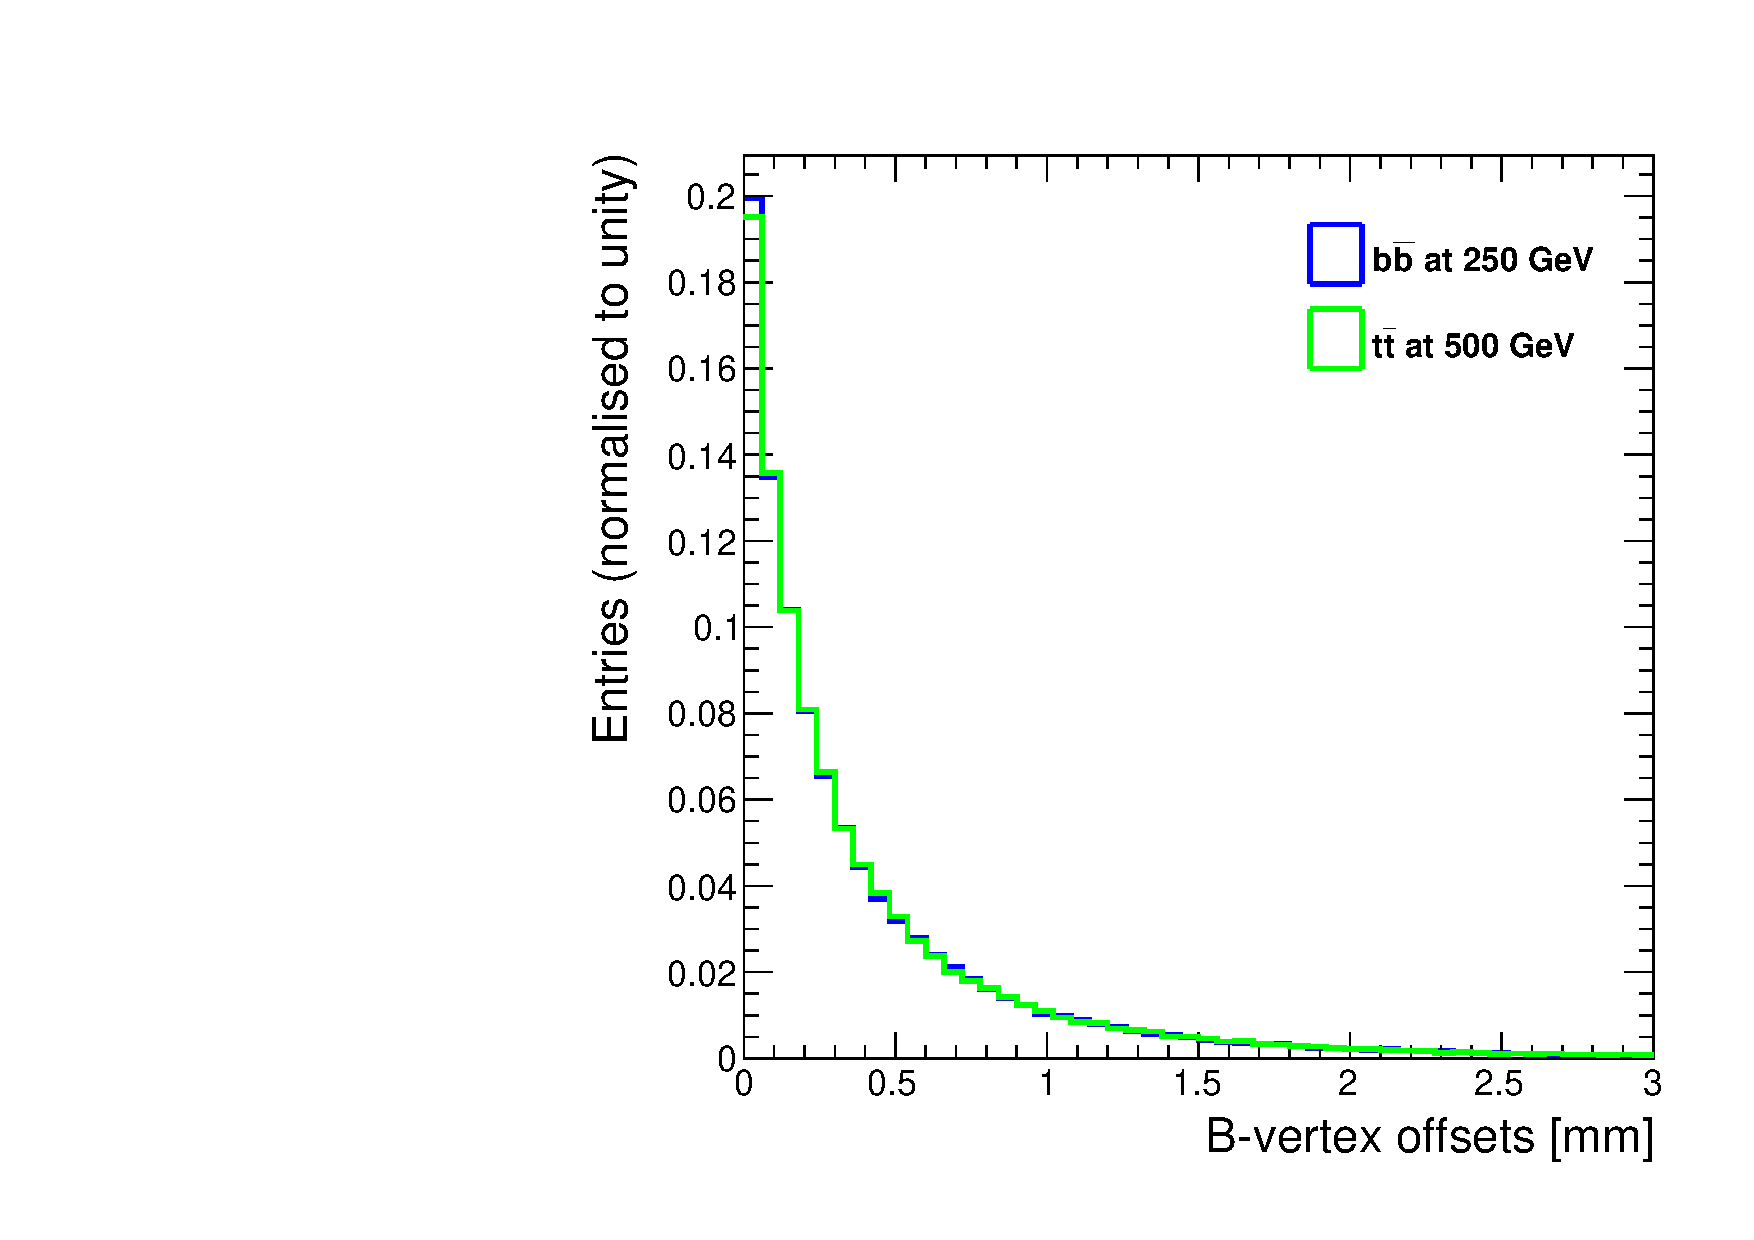
\includegraphics[width=0.95\textwidth]{ILD/plots/gen-bvtx-offsets.pdf}
\caption{\label{fig:GenVtxOffset_a_3} }
\end{subfigure}% 
  \begin{subfigure}{0.5\textwidth}
\centering
    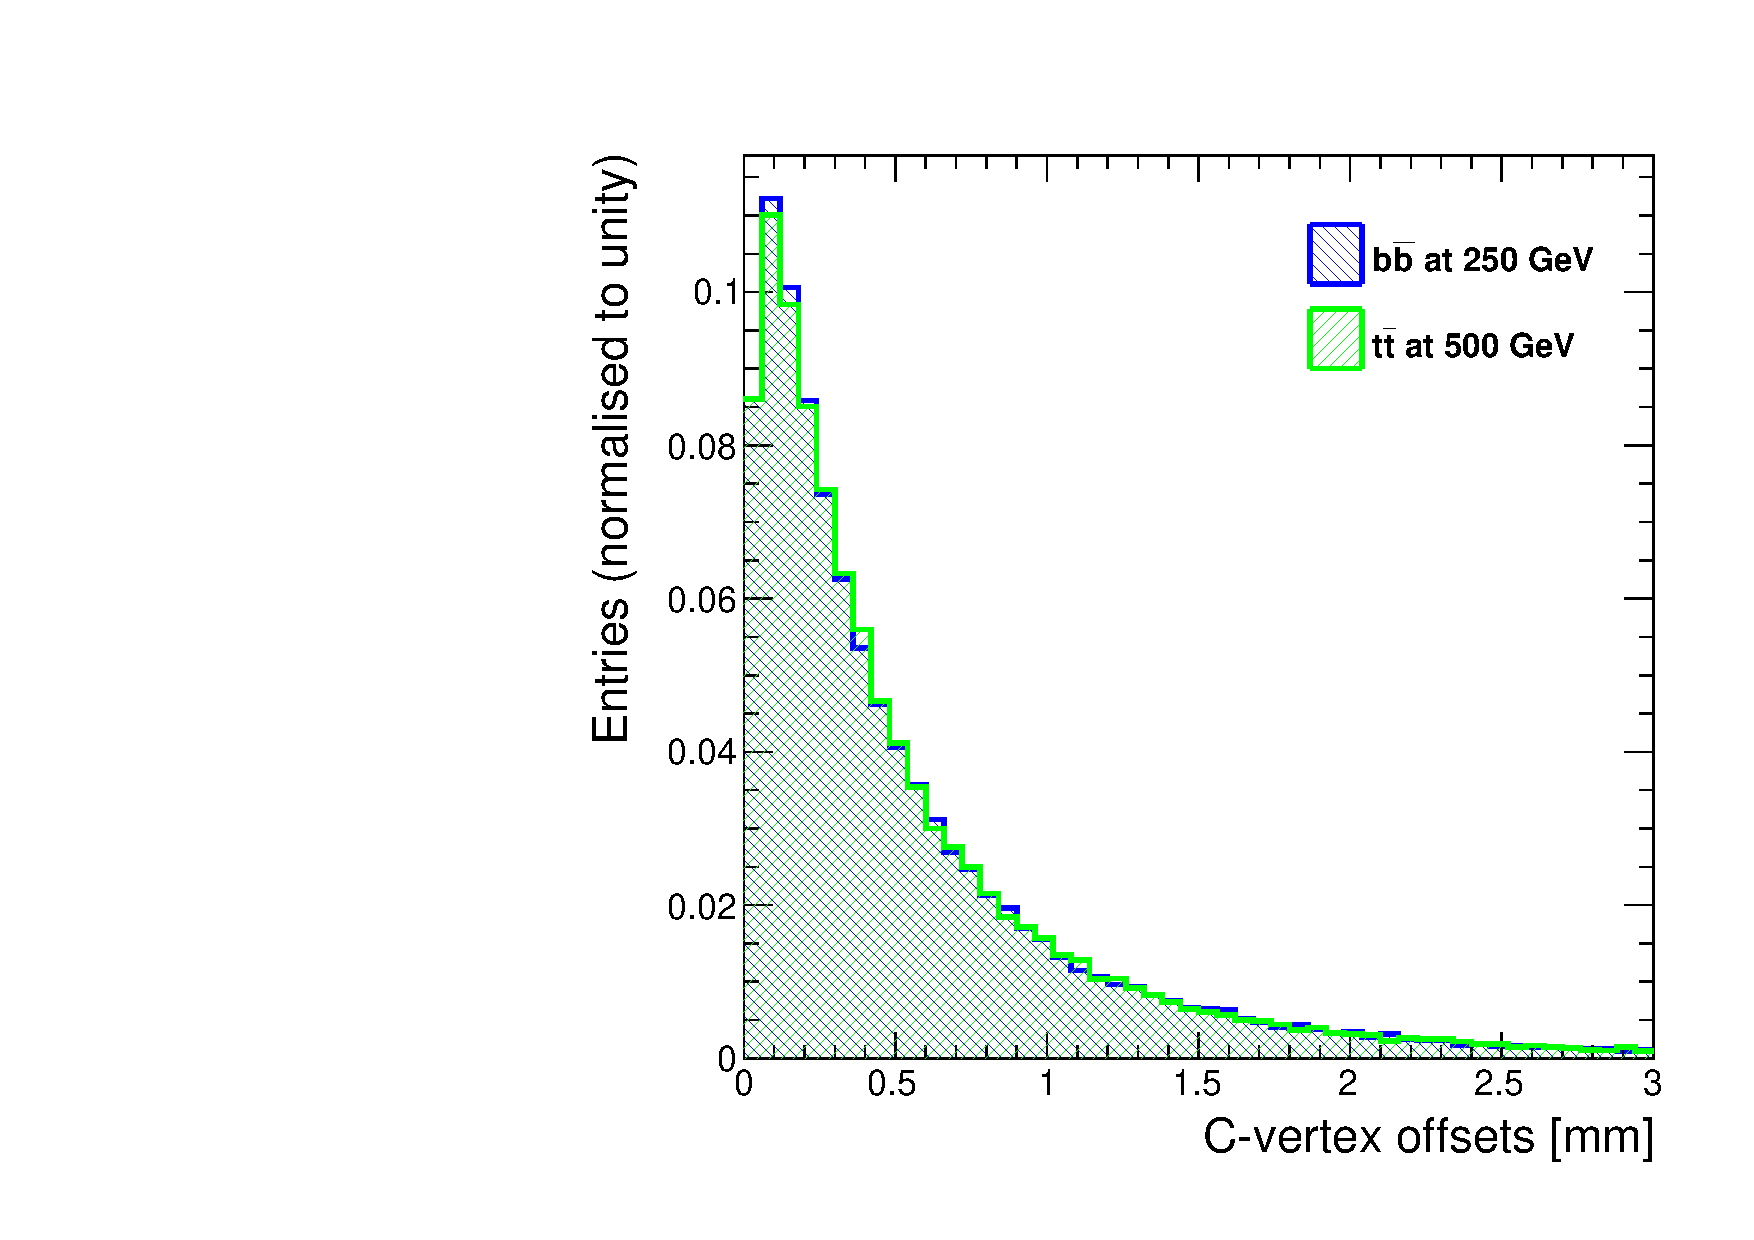
\includegraphics[width=0.95\textwidth]{ILD/plots/gen-cvtx-offsets.pdf}
\caption{\label{fig:GenVtxOffset_b_3} }
\end{subfigure}
    \caption{\sl Distributions of the b-vertex (a) and c-vertex prong offsets~(b). }
    \label{fig:GenVtxOffset_3}
\end{figure}

The distributions of the total charge multiplicity and the flight distance of the b-hadrons are displayed in Fig.~\ref{fig:GenHadronParams_3}.
The imbalance between the odd and even number of multiplicities is caused by the presence of the \Bzs\ hadronization modes.

Regarding the similarity of the distributions for two processes shown in Figures ~\ref{fig:GenVtx_3}, \ref{fig:GenHadronParams_3} and \ref{fig:GenVtxOffset_3}, the performance of a vertexing algorithm should be identical for the same energy and the direction of the b-hadron decays.


\begin{figure}[h]
\centering
\begin{subfigure}{0.5\textwidth}
    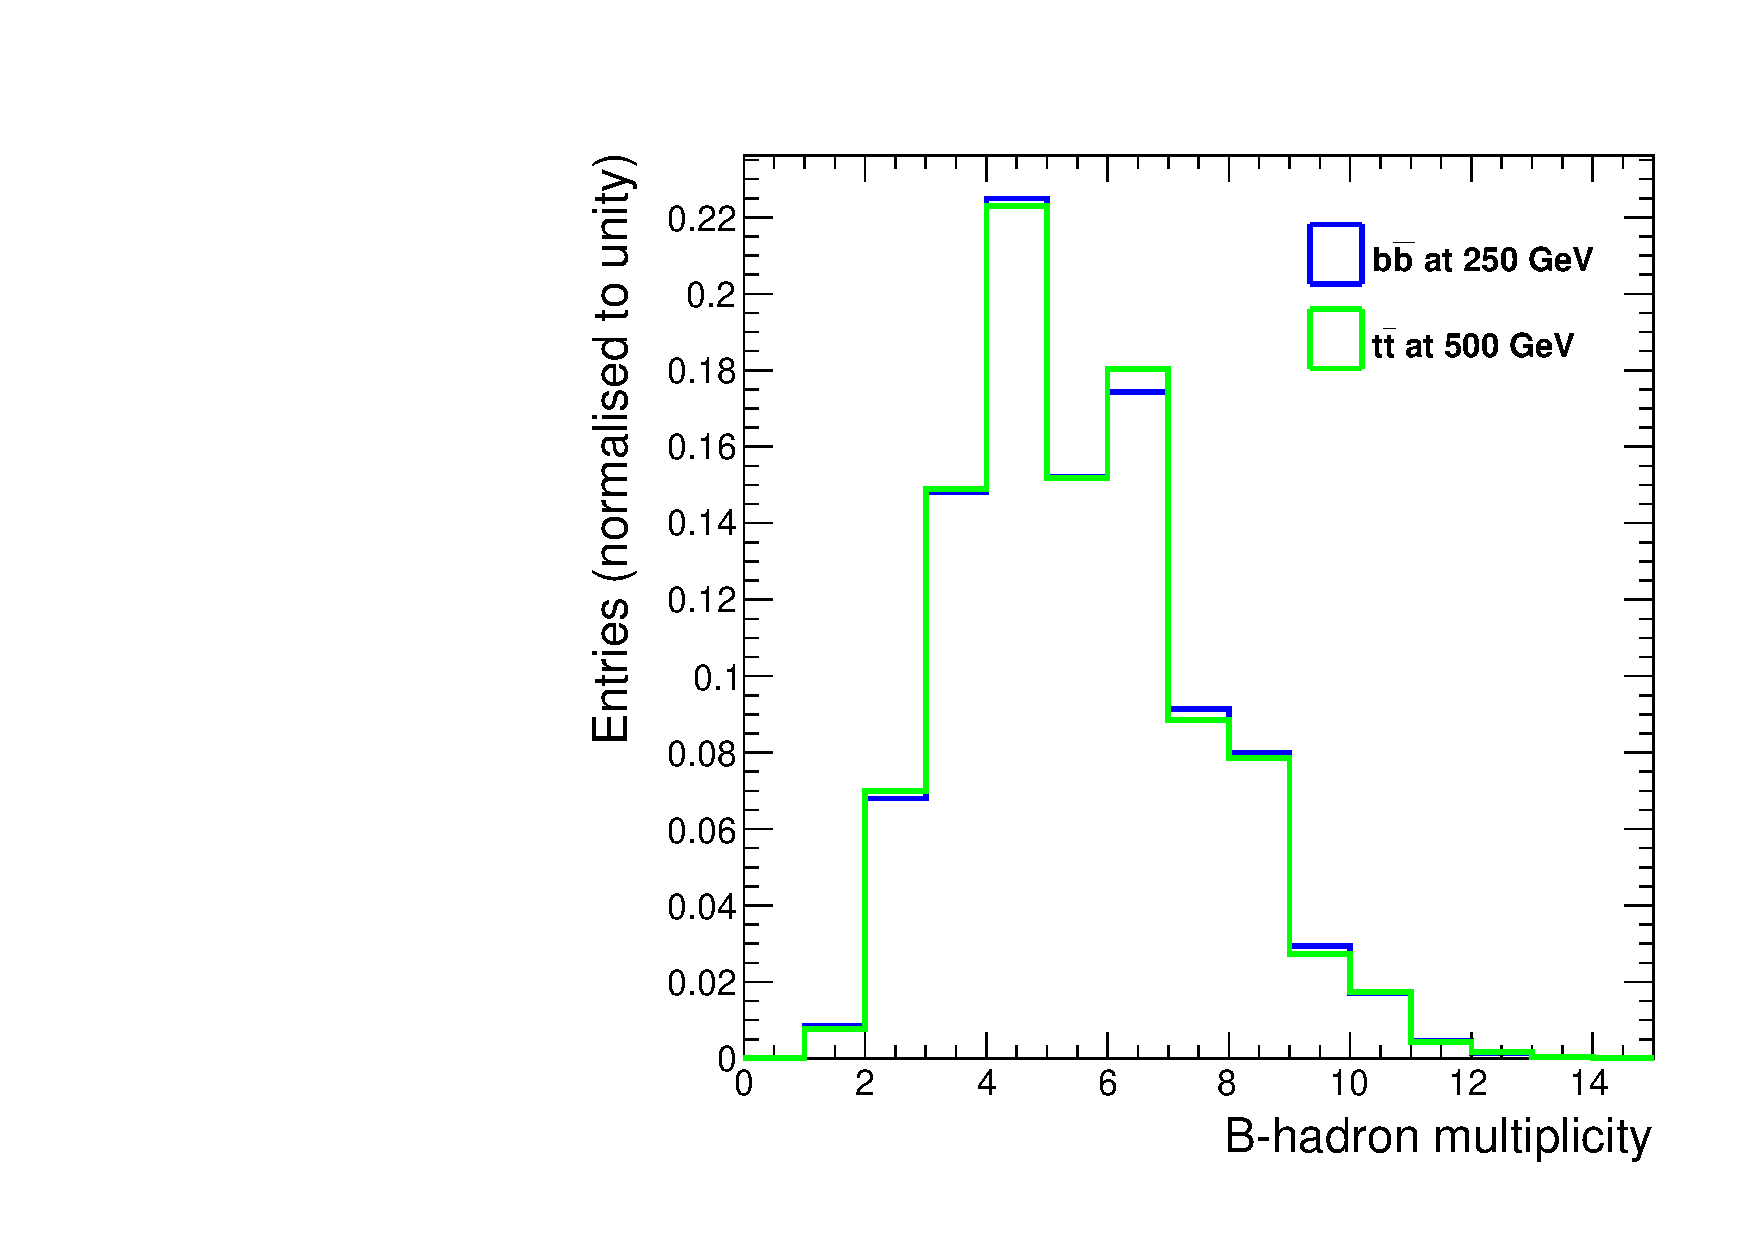
\includegraphics[width=0.95\textwidth]{ILD/plots/gen-hadron-multiplicity.pdf}
\caption{\label{fig:GenHadronParams_a_3} }
\end{subfigure}% 
  \begin{subfigure}{0.5\textwidth}
\centering
    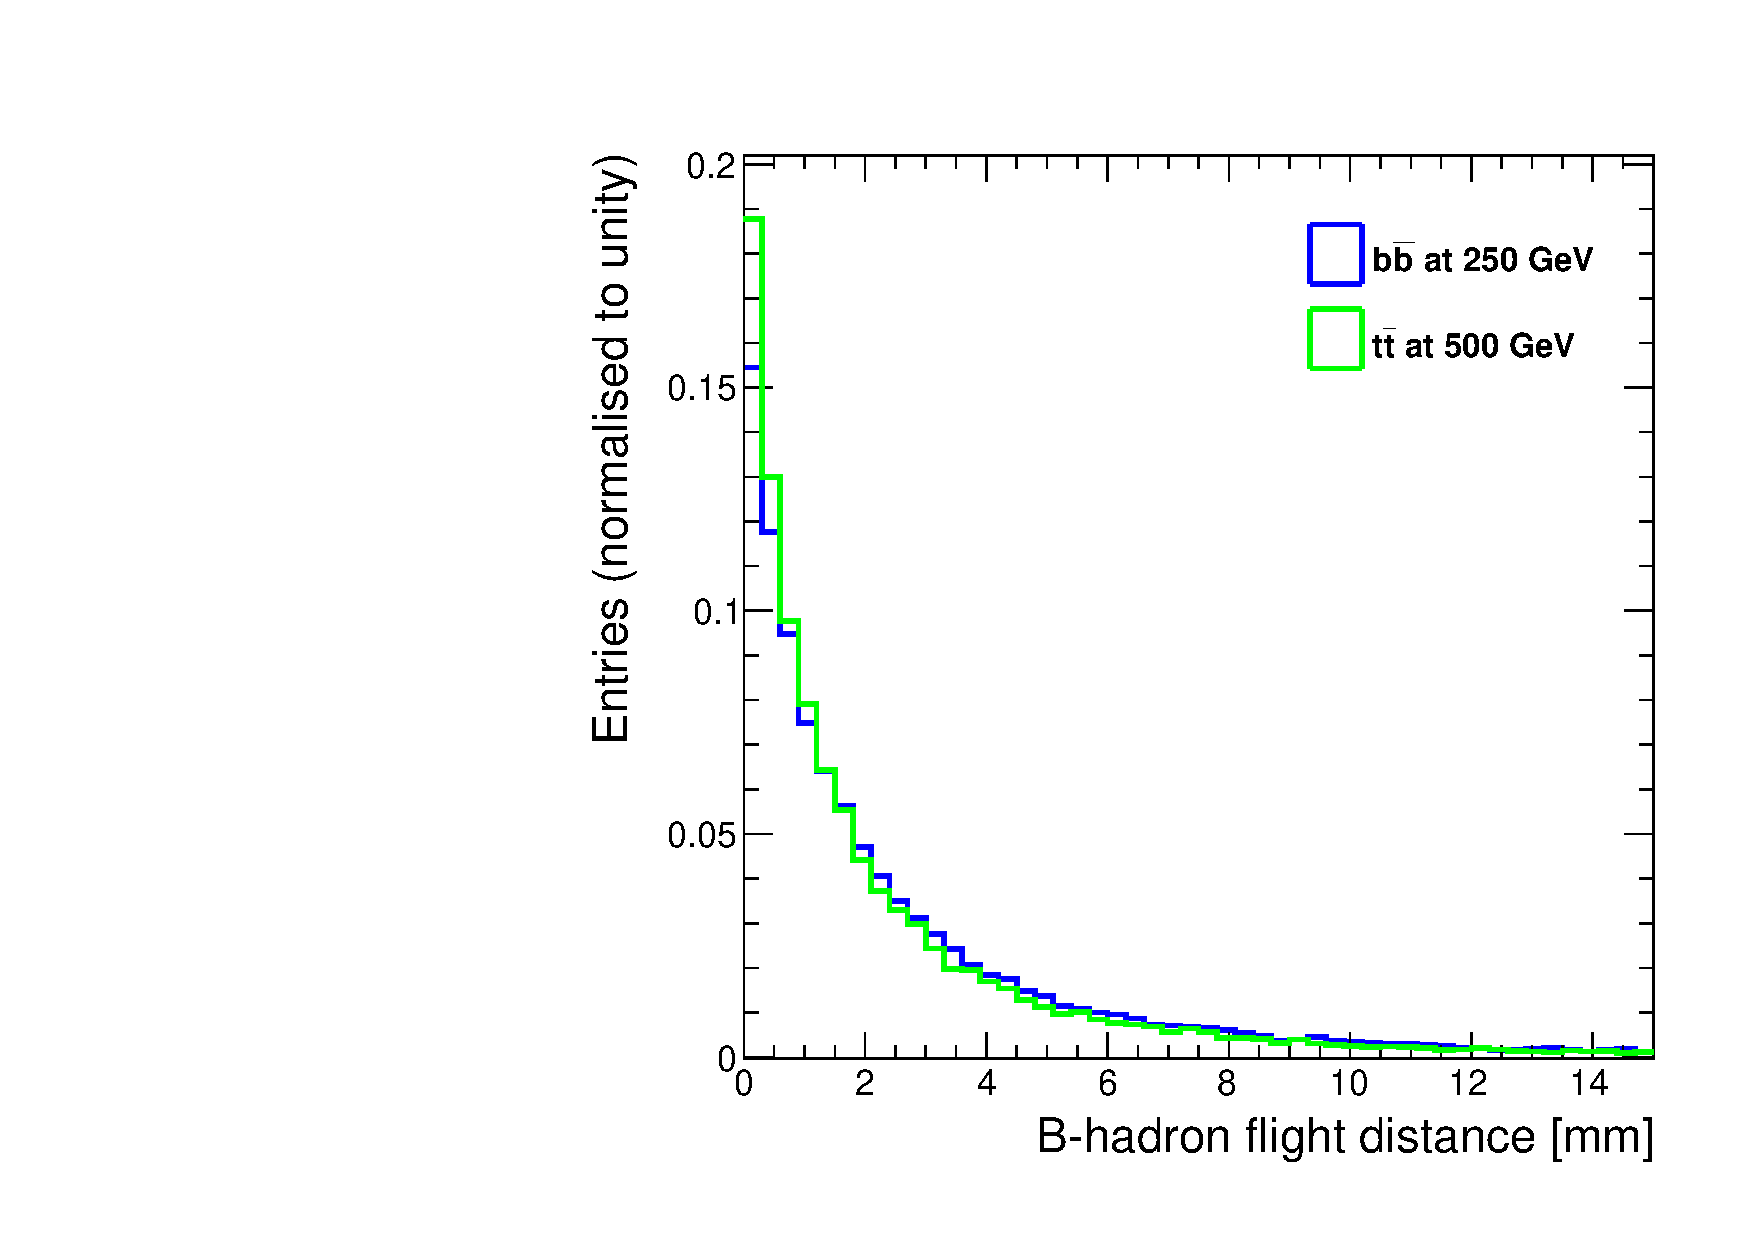
\includegraphics[width=0.95\textwidth]{ILD/plots/gen-hadron-distance.pdf}
\caption{\label{fig:GenHadronParams_b_3} }
\end{subfigure}
    \caption{\sl Left: Distribution of the b-hadron charge multiplicity. The odd multiplicities correspond to the charged hadrons and the even multiplicities correspond to the neutral hadron decays.   Right: Distribution of the b-hadron distance of flight. }
    \label{fig:GenHadronParams_3}
\end{figure}

One can look for the charged kaons among the generated prongs of the b-hadrons and study the charge correlation between $K^\pm$ charge and initial b-hadron charge. Figure~\ref{fig:KaonOscillation_3} shows, that the neutral b-hadrons have higher chances to produce $K^\pm$ with an opposite charge to the parent b-hadron, which means that the $B^0-\bar{B}^0$ oscillations are enabled in {\sc pythia} event generator.

\begin{figure}[h]
{\centering
    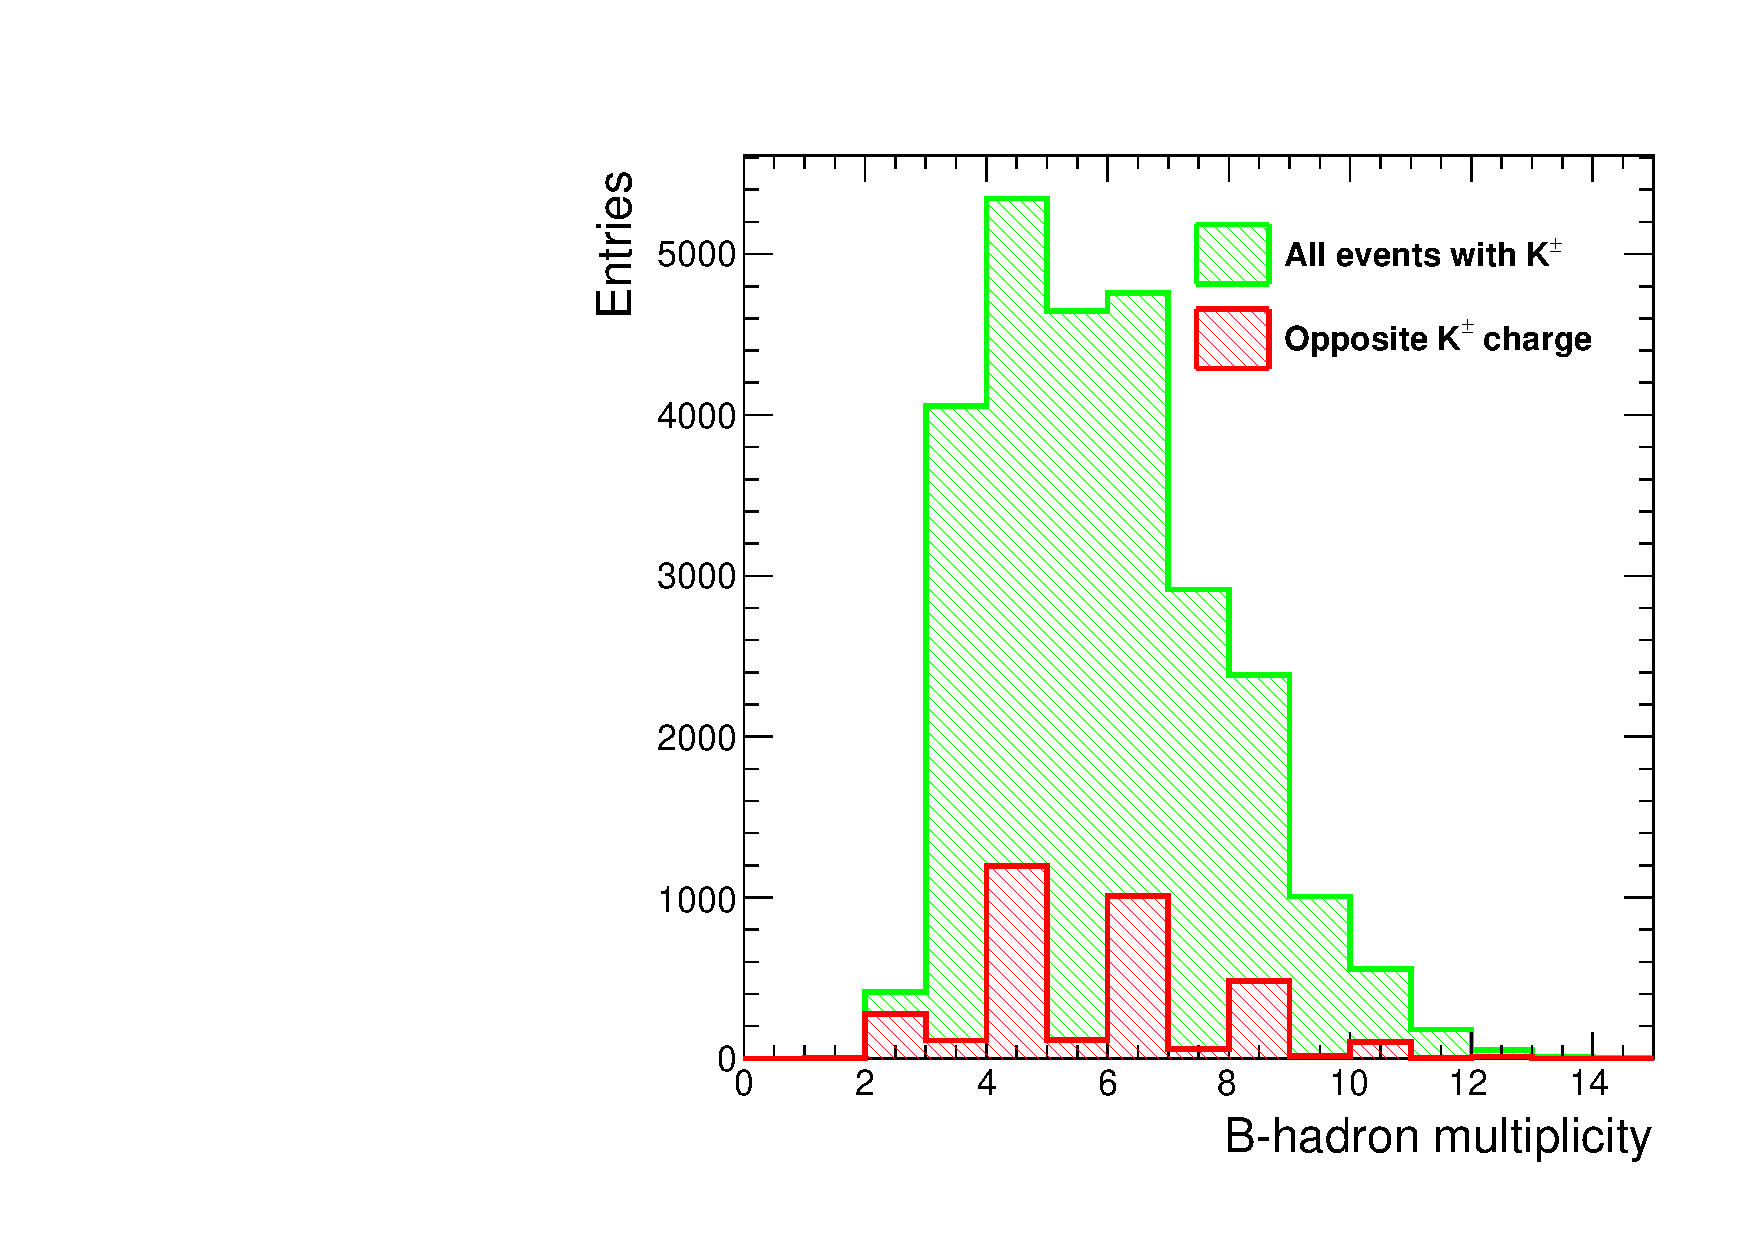
\includegraphics[width=0.45\textwidth]{ILD/plots/kaon-oscillation.pdf}
    \caption{\sl The multiplicity of all b-hadrons with a $K^\pm$-meson among the generated prongs (green) and the multiplicity of b-hadrons with $K^\pm$ of opposite charge to b-hadron charge (red).
    }
    \label{fig:KaonOscillation_3}
  }
\end{figure}

About 87\% of b-hadrons are set to have correlated $K^\pm$ charge in the generator, which makes the $K^\pm$ charge a reliable indication of the initial b-quark charge.
%The design of the ILD vertex detector is optimized to have the best offset resolution 

%%%%%%%%%%%%%%%%%%%%%%%%%%%%%%%%%%%%%%%%%%%%%%%%%%%%%%%%%
%%%%%%%%%%%%%%%%%%%%%%%%%%%%%%%%%%%%%%%%%%%%%%%%%%%%%%%%%
%%%%%%%%%%%%%%%%%%%%%%%%%%%%%%%%%%%%%%%%%%%%%%%%%%%%%%%%%

\subsection{Baseline vertex reconstruction}
The LCFI+ package finds the secondary and tertiary vertices and tags the b- and c-jets using the final reconstructed charged particles, the Particle Flow objects.
It has several stages of the vertex reconstruction and flavor-tagging, which are implemented in the following algorithms:
\begin{itemize}
\item PrimaryVertexFinder finds the position of the primary interaction point and the corresponding charged particles;
\item BuildUpVertex forms the reconstructed vertex candidates, which can have two or more associated charged particles, referred in text as reconstructed prongs;
\item JetVertexRefiner finds vertices with only one prong using the reconstructed vertex candidates and it organizes the vertex candidates into maximum two reconstructed vertices per jet.
\item FlavorTag algorithm calculates b-tag and c-tag values for a jet, using the finalized jet vertices from the JetVertexRefiner.
\end{itemize}

In this section, only the standard reconstruction chain is used to study the b-jet charge measurement. 

%%%%%%%%%%%%%%%%%%%%%%%%%%%%%%%%%%%%%%%%%%%%%%%%%%%%
%%%%%%%%%%%%%%%%%%%%%%%%%%%%%%%%%%%%%%%%%%%%%%%%%%%%
%%%%%%%%%%%%%%%%%%%%%%%%%%%%%%%%%%%%%%%%%%%%%%%%%%%%
\subsubsection{Baseline jet charge reconstruction}
The jet charge can be computed as a sum of the reconstructed particles charges, associated to the reconstructed vertices, which belong to a given jet. 
Therefore, the vertexing algorithm should correctly associate all secondary or tertiary vertex particles to have a correct jet charge measurement. 
The correctly reconstructed jet charge should have the same sign of charge as the generated charged b-hadron or it should have reconstructed zero charge if the generated b-hadron is neutral. 
Regarding the b-hadron multiplicity, shown in Fig.~\ref{fig:GenHadronParams_3}, this task is not trivial. 


The charge purity $P_B$ is defined to be the number of correctly reconstructed jet charges divided by the total number of jets. 
The previous studies done in the fully hadronic $t\bar{t}$ decays~[Amjad] have shown that the total jet charge purity $P_B$ is about 60\%.
The total jet charge for the considered $b\bar{b}$ process  is $P_B(b\bar{b}) = 66\%$ and for semileptonic decay of the  $t\bar{t}$ pair is $P_B(t\bar{t}) = 64\%$. 
The small difference between these values is caused mostly by the difference in the generated momentum  distributions displayed in Fig.~\ref{fig:GenHadronMomentum_3} and by the difference in the jets environments.

Using the output of the TruthVertexFinder, one can compare the generated vertices with the corresponding reconstructed vertices, detected by the LCFI+ algorithms. 
The number of the generated prongs $N_{gen}$ can be compared to the number of the reconstructed prongs $N_{rec}$ on the jet-per-jet basis as it is shown in Fig.~\ref{fig:Table_3}. 
The jets, which have no associated reconstructed vertices, will cause the efficiency decrease in the jet charge measurement, however, they have no influence on the method purity.
The jets with reconstructed vertices have the following statistics:
\begin{itemize}
\item Only 49\% of these jets are perfectly reconstructed and have $N_{rec}=N_{gen}$;
\item The 46\% of the jets have lost one or more prongs from the reconstructed vertices having $N_{rec}<N_{gen}$;
\item The rest 5\% are the jets with vertices, contaminated by particles with non b-hadron origin and have $N_{rec}>N_{gen}$.
\end{itemize}

\begin{figure}[h]
{\centering
    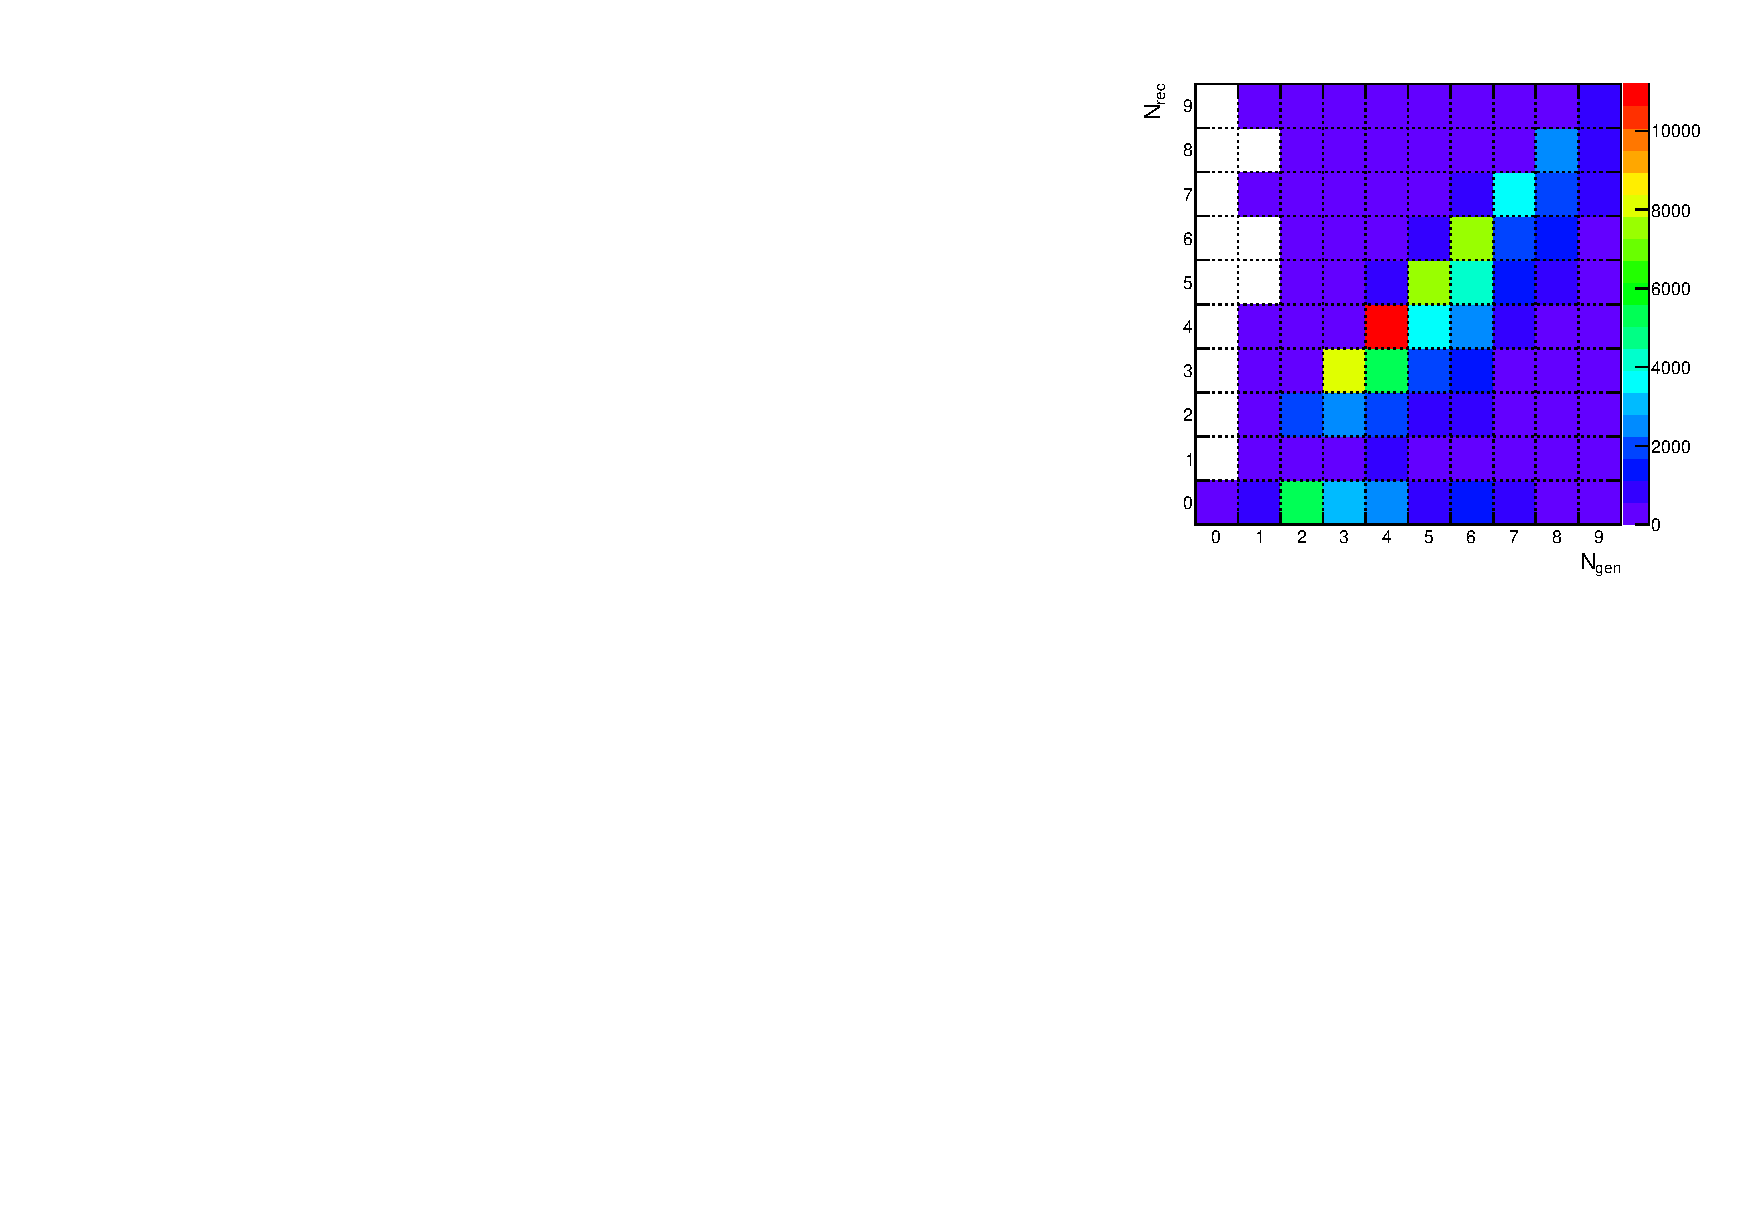
\includegraphics[width=0.55\textwidth]{ILD/plots/rec-gen-table.pdf}
    \caption{\sl Comparison of the number of reconstructed tracks $N_{gen}$ to the number of generated tracks $N_{rec}$ for a given b-jet. The number of entries is color-coded for each cell. The diagonal has 49\% of all entries and it contains the jets, which have the correctly reconstructed vertices. The b-jets below diagonal have vertices with one or more particles missed by reconstruction. The row $N_{rec} = 0$ corresponds to the b-jets with no reconstructed vertices. %Right: Same comparison, but after a cut on the b-tag$> 0.8$ and a cut on the b-hadron momentum more than 20\,GeV. The diagonal contains 55\% of the jets after the cuts.
    }
    \label{fig:Table_3}
  }
\end{figure}

The jets with $N_{rec}=N_{gen}$ have the charge purity of more than 97\%, while all other jets have an almost random reconstructed jet charge with the corresponding charge purity about 35\%. 
Hence, the purity reduction is mainly caused by the jets, which have lost the prongs from their reconstructed vertices. 
The application of cuts, for example on jet b-tag$>0.8$ and reconstructed b-hadron momentum $|p_{had}| > 20$\,GeV, increases the fraction of correctly reconstructed jets up to 55\%, however with an efficiency penalty of 17\%.
The cuts on the b-tag value are necessary to reject background processes and will be adjusted to archieve the best background suppression. 

The fraction of entries above diagonal in Fig.~\ref{fig:Table_3} is small, comparing to the fraction of events above the diagonal. 
Therefore, there is a possibility to develop a recovery algorithm, which can add the missing prongs to the reconstructed vertices, with a slight increase of the number of jets with contaminated vertices. 
But first, one needs to study the reasons behind the missing prongs and analyze the possibility to recover them. 

%%%%%%%%%%%%%%%%%%%%%%%%%%%%%%%%%%%%%%%%%%%%%%%%%%%%
%%%%%%%%%%%%%%%%%%%%%%%%%%%%%%%%%%%%%%%%%%%%%%%%%%%%
%%%%%%%%%%%%%%%%%%%%%%%%%%%%%%%%%%%%%%%%%%%%%%%%%%%%
\subsubsection{Missing vertices}
The reconstruction algorithm can lose a vertex if the generated b-hadron properties, like number of generated prongs, b-hadron momentum or polar angle, are in the poor acceptance of the detector. 
The non-reconstructed vertices contain approximately 22\% of all generated b-hadron prongs. 
The b-hadron vertices with generated low momentum prongs or low offset prongs have higher chances to be missed by the reconstruction algorithms. 
The distributions of the average prong offset and momentum for reconstructed vertices and missed vertices are shown in Fig.~\ref{fig:RecMissedParams_3}. 
On can conclude, that the reconstruction algorithms start to lose their efficiency at below 4\,GeV average prong momentum and below 0.5\,mm average prong offset. 

\begin{figure}[h]
\centering
\begin{subfigure}{0.5\textwidth}
    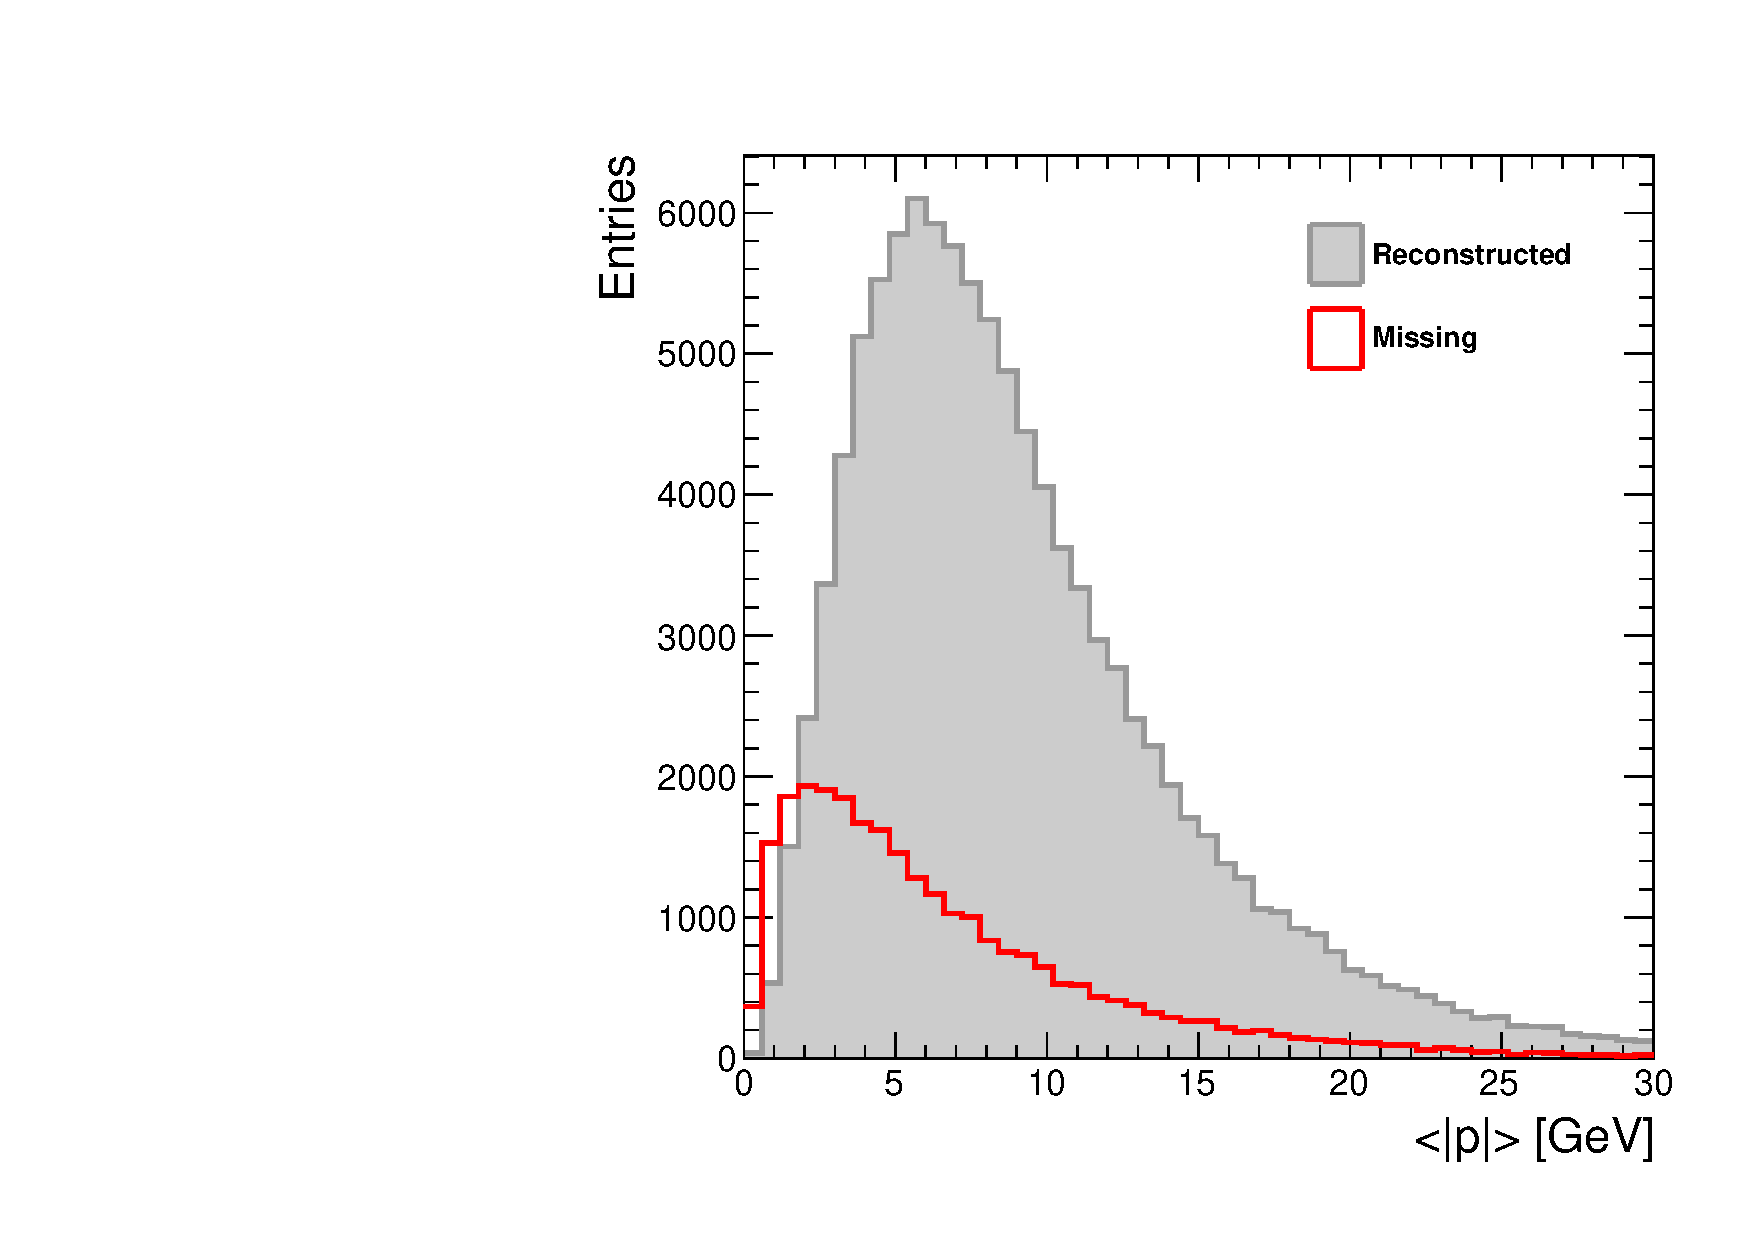
\includegraphics[width=0.95\textwidth]{ILD/plots/rec-missed-p-vtx.pdf}
\caption{\label{fig:RecMissedParams_a_3} }
\end{subfigure}% 
  \begin{subfigure}{0.5\textwidth}
\centering
    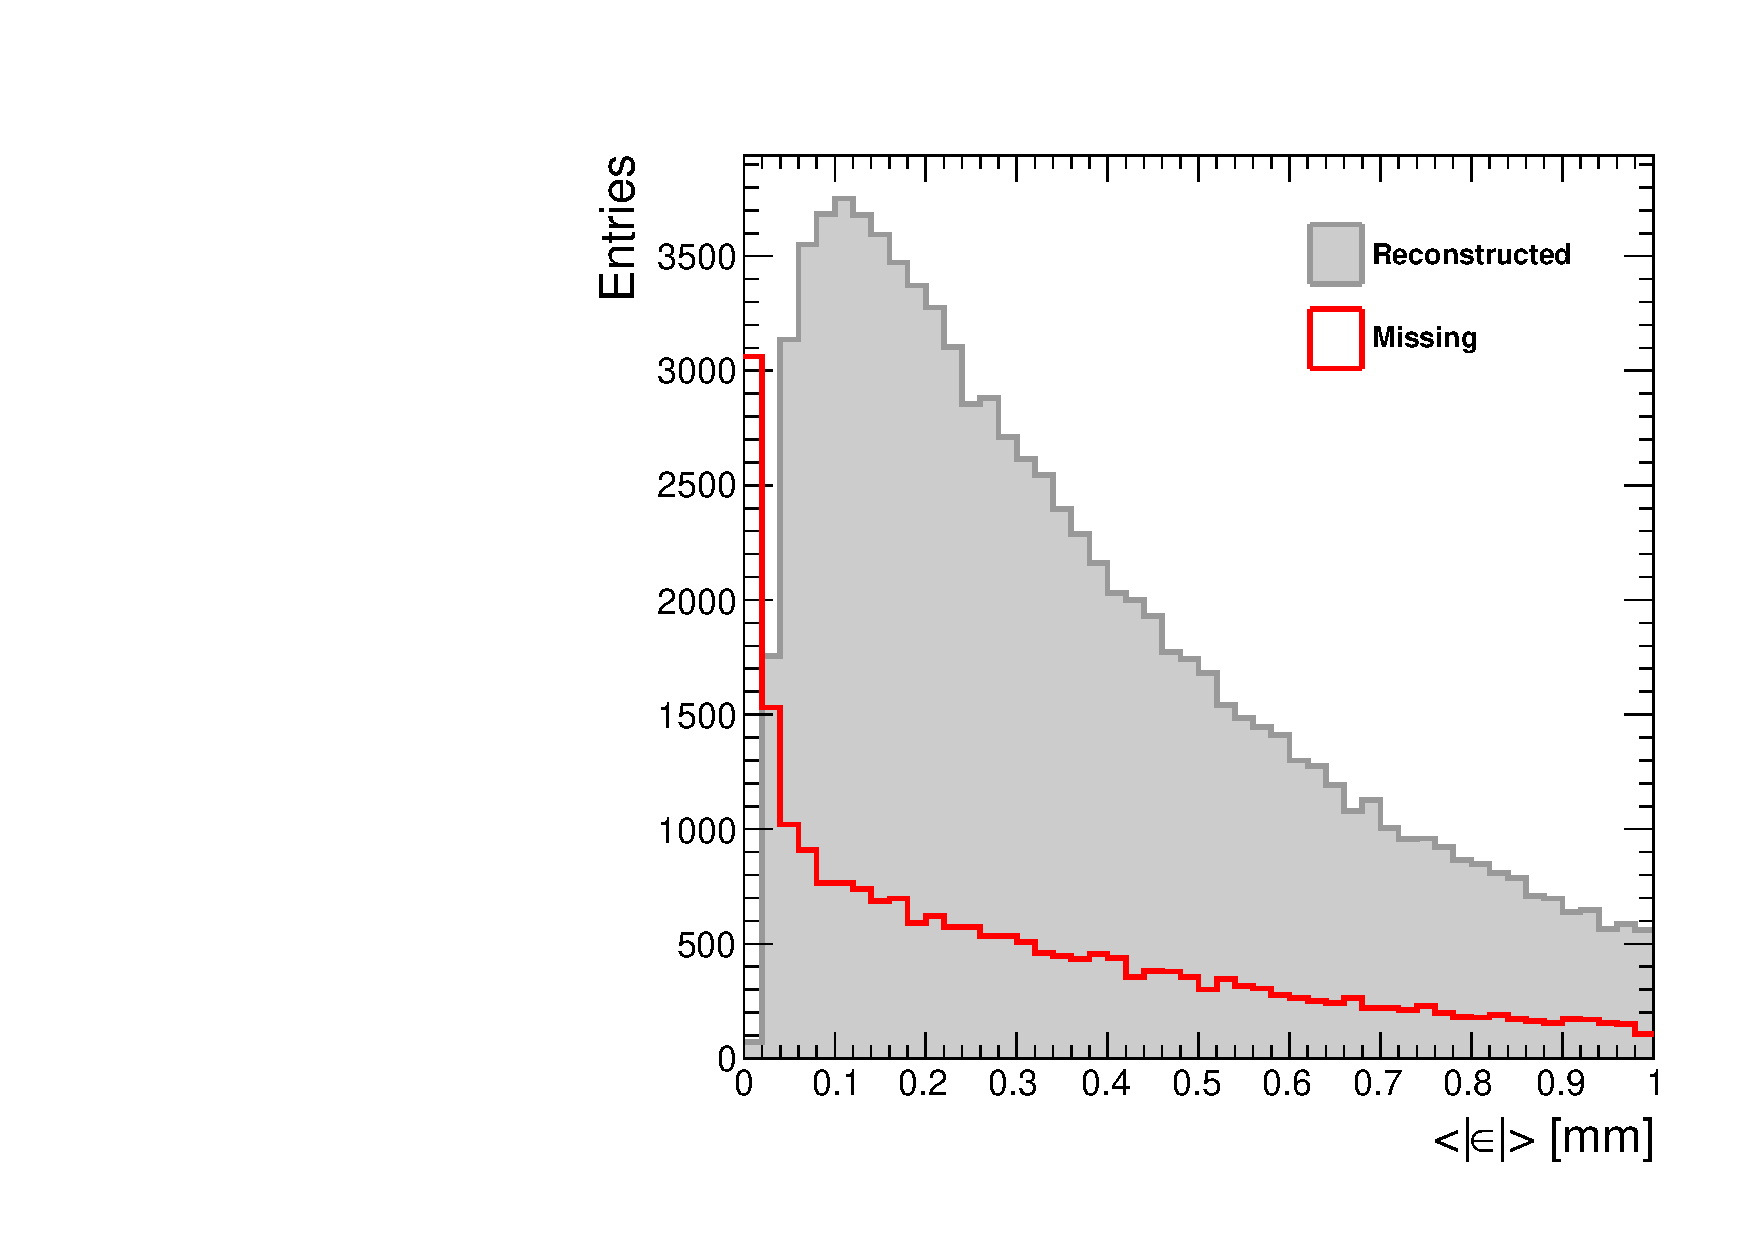
\includegraphics[width=0.95\textwidth]{ILD/plots/rec-missed-s-vtx.pdf}
\caption{\label{fig:RecMissedParams_b_3} }
\end{subfigure}
    \caption{\sl Distributions of the average prong momentum~(a) and offset (b) of the missed and reconstructed vertices. }
    \label{fig:RecMissedParams_3}
\end{figure}

\begin{figure}[h]
{\centering
    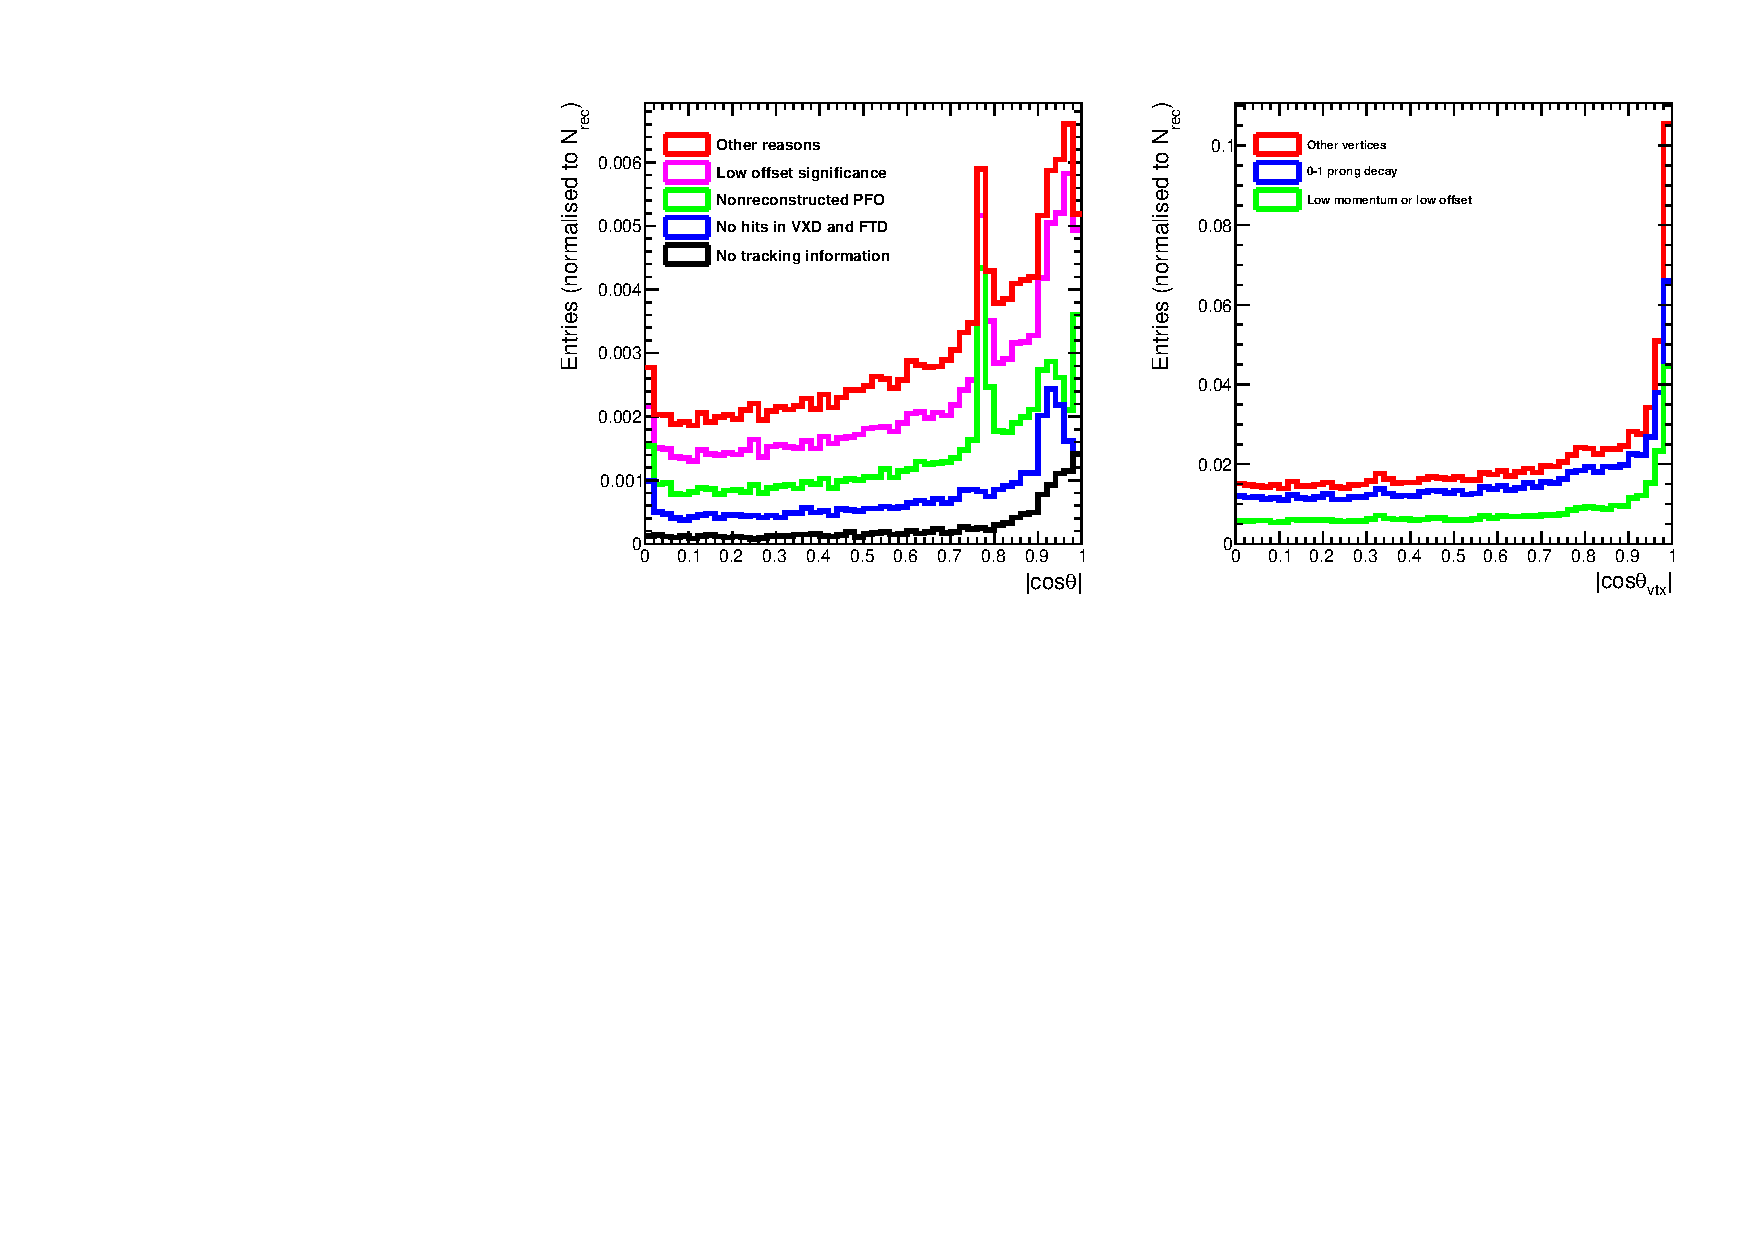
\includegraphics[clip, trim=10.cm 0cm 0.cm 0cm, width=0.55\textwidth]{ILD/plots/missed-cos-vtx.pdf}
    \caption{\sl Polar angle distribution of the missed vertices subdivided into different categories. This is a stacked histogram. The low momentum or low offset category are the missing vertices, which have the average prong momentum below  4\,GeV or below 0.5\,mm average prong offset.
    }
    \label{fig:MissedCos_3}
  }
\end{figure}

The polar angle distributions of the missing vertices is displayed in Fig.~\ref{fig:MissedCos_3}. 
One can summarize the reasons to not reconstruct a vertex as following: 
\begin{itemize}
\item Neutral decay vertex - vertex cannot be reconstructed if it has no generated prongs;
\item Low energy of the generated b-hadron - cause a low flight distance, low offsets or low momentum of the generated prongs, which makes difficult to separate out the b-hadron prongs from the other particles in a b-jet;
\item One prong decay vertex can be lost if there was no other vertices reconstructed in a given b-jet;
\item The most of the b-hadrons, produced in the forward region, or outside the barrel VXD acceptance $|\cos\theta_{vtx}| > 0.95$, are not reconstructed, which is a reason of a low precision on the impact parameters of the reconstructed prongs. 
\item "Higgs-like" increase at $|\cos\theta_{vtx}| \approx 0.8$ is discussed in Sec.~\ref{sec:MissingProngs}.
\end{itemize}

An attempt was made to reduce the vertexing inefficiency in the forward region

The missing vertices are difficult to recover, however they have essentially no impact on the jet charge purity, therefore the further studies are focused on the missing prongs of the reconstructed vertices.
%%%%%%%%%%%%%%%%%%%%%%%%%%%%%%%%%%%%%%%%%%%%%%%%%%%%
%%%%%%%%%%%%%%%%%%%%%%%%%%%%%%%%%%%%%%%%%%%%%%%%%%%%
%%%%%%%%%%%%%%%%%%%%%%%%%%%%%%%%%%%%%%%%%%%%%%%%%%%%
\subsubsection{Missing prongs from the reconstructed vertices}
\label{sec:MissingProngs}
The quality of vertex reconstruction strongly depends on all reconstruction algorithms as well as on various geometry aspects of the ILD experiment. 

%Using TruthVertexFinder information and truth links to the reconstructed particles, one can find, that the 
The missing reconstructed prongs are approximately 10.4\% of the total generated prongs for the baseline vertex reconstruction. 
A detailed study was made to reveal the reasons behind the missing prongs, which can be summarized as follows:
\begin{itemize}
\item No tracking information - the MarlinTrk algorithms failed to reconstruct the track. This category is tiny - only 0.93\% of the generated prongs;
\item No associated hits in the VXD or FTD - the track segment from the Vertex Detector or Forward Tracking Discs was not connected to the large TPC track segment. Such reconstructed particles have uncertainties on the impact parameters, which makes them not suitable for vertexing algorithms. They are 2.\% of the generated prongs;
\item No reconstructed PFO - the PandoraPFO failed to create the PFO from a reconstructed track, which makes it not usable for LCFI+ algorithms - 3.2\%  of the generated prongs;
\item Low generated momentum $|p|$ or offset $\epsilon$ - the reconstructed particle was produced with impact parameters below the detector resolution - 3.1\%  of the generated prongs;
\item Other reasons, mostly because of the vertex fitting problems - 1.7\% of the generated prongs.
\end{itemize}



\begin{figure}[h]
\centering
\begin{subfigure}{0.5\textwidth}
    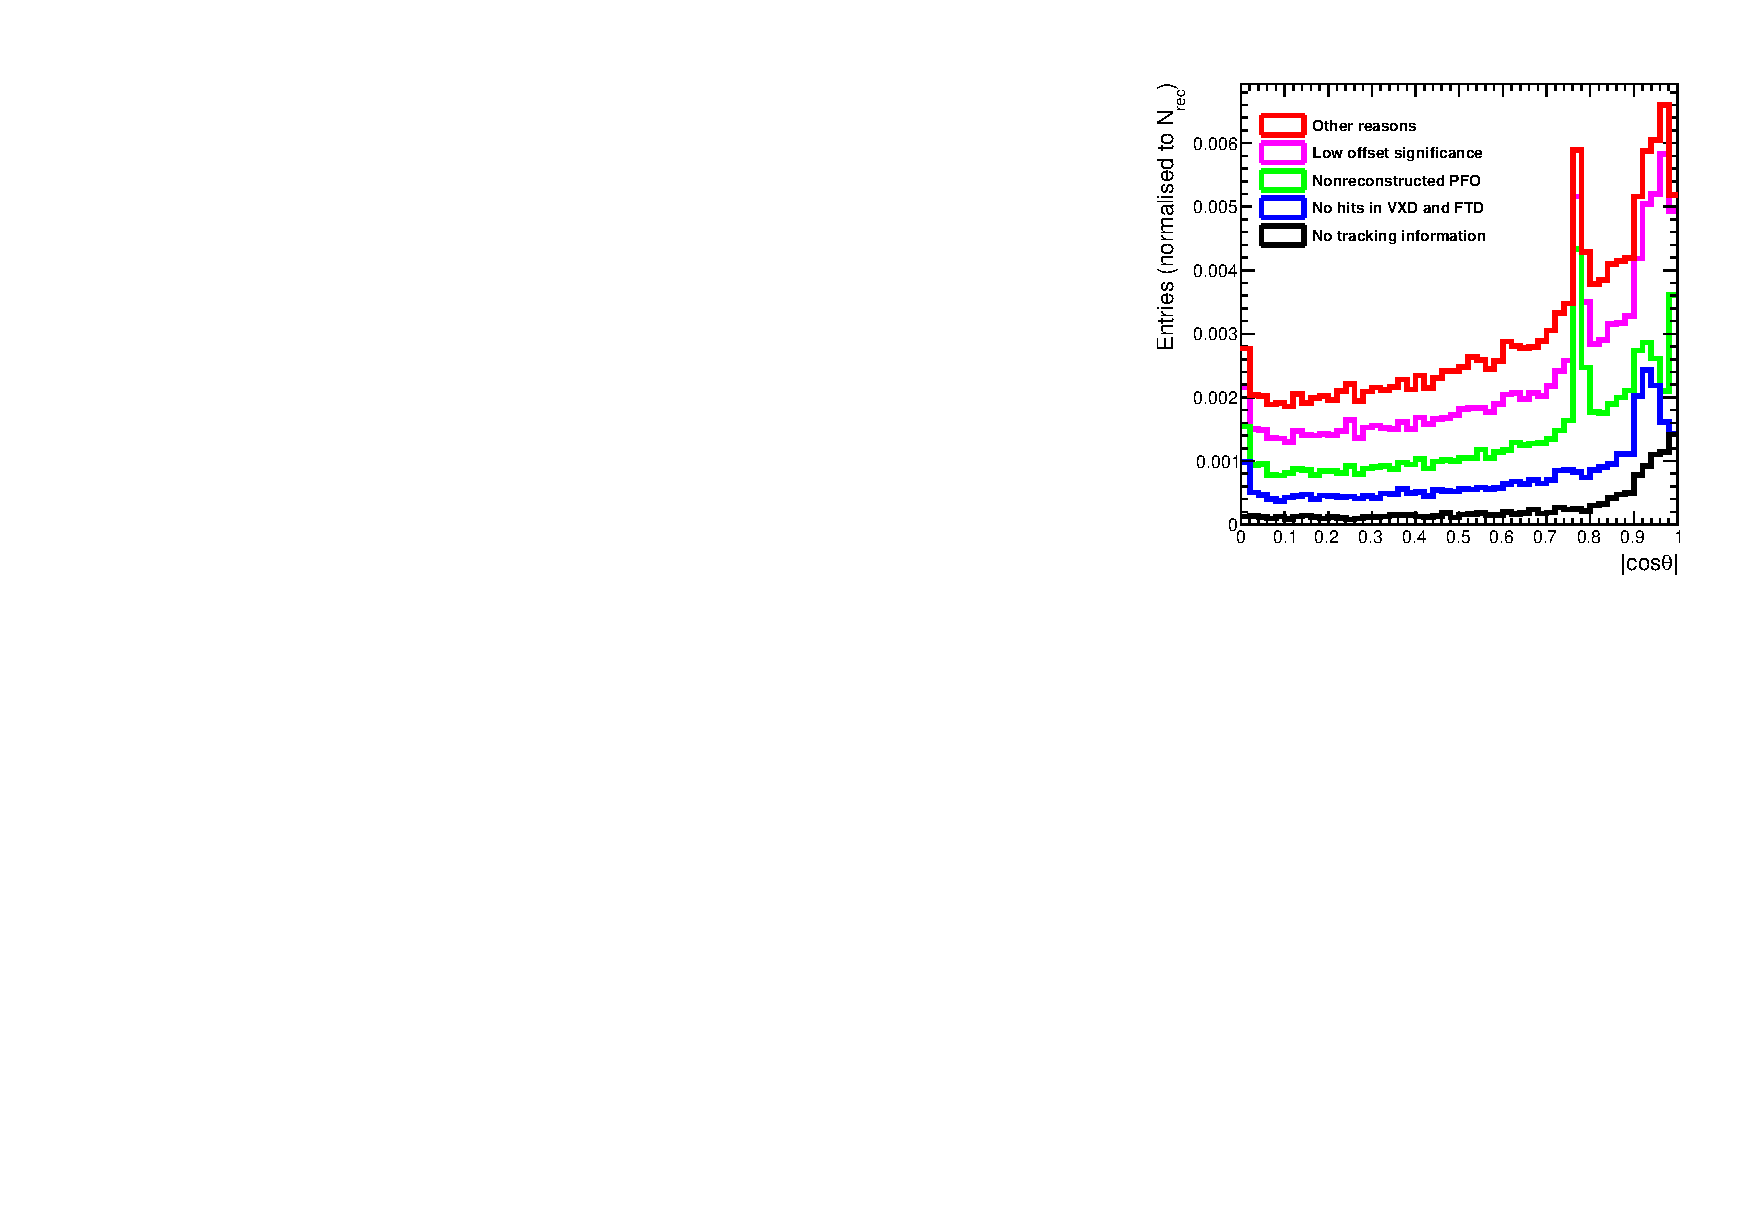
\includegraphics[width=0.95\textwidth]{ILD/plots/missed-tracks.pdf}
\caption{\label{fig:MissingTracks_cos_3} }
\end{subfigure}% 
  \begin{subfigure}{0.5\textwidth}
\centering
    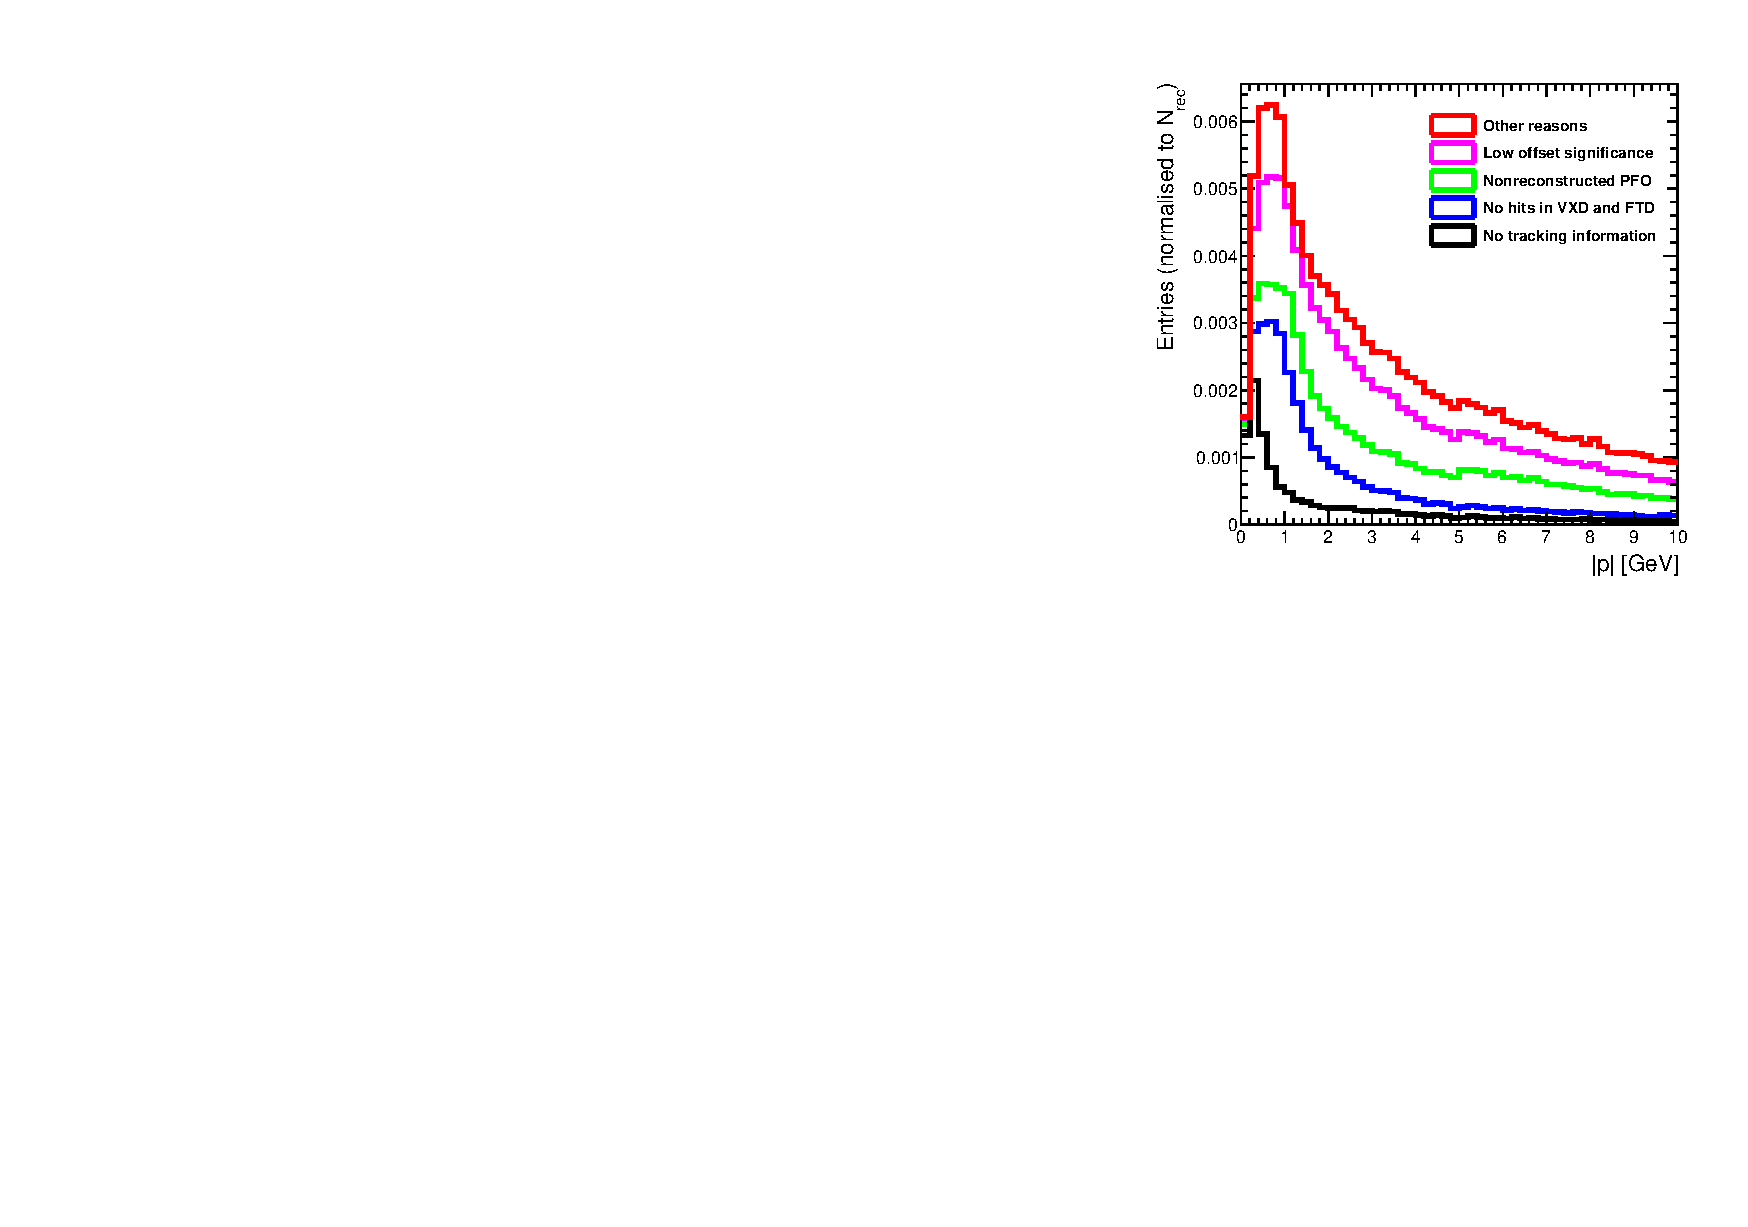
\includegraphics[width=0.95\textwidth]{ILD/plots/missed-momentum.pdf}
\caption{\label{fig:MissingTracks_p_3} }
\end{subfigure}
    \caption{\sl Polar angle~(a) and momentum~(b) distributions of the missing prongs subdivided into different categories. This is a stacked histogram. The peak at $|\cos\theta| \approx 0 $ is caused by the gap between TPC endplates, the peak at  $|\cos\theta| \approx 0.8$ is caused by barrel-endcap transition in the \ecal\ and the rapid increase at $|\cos\theta| \approx 0.9$ is caused by the barrel-endcap transition in the VXD and FTD system. }
    \label{fig:MissingTracks_3}
\end{figure}

These categories of the missing prongs can be illustrated on the polar angle histogram, shown in Fig.~\ref{fig:MissingTracks_3}, which also reveals the following problems connected to the ILD geometry:
\begin{itemize}
\item Small peak at $|\cos\theta| \approx 0$ is caused by the insensitive gap between the TPC endplates, which induce a problem with a connection between the VXD track segments and the reduced TPC track segment;
\item Large peak at $|\cos\theta| \approx 0.8$ is caused by the PandoraPFO, which fails to connect a well reconstructed track with an offset to a segmented cluster situated in the \ecal\ barrel-endcap transition. This problem is specific to the b-hadron tracks;
\item Increase at $|\cos\theta| \approx 0.9$ correspond to the end of the full 3 double layer VXD acceptance, which cause an increase in the impact parameter uncertainties of the reconstructed tracks. %caused by a connection problem between the VXD track segments, which are in the acceptance region of the two double-sided VXD layers, and the FTD track segments.
\end{itemize}

The recoverable prongs are the ones, which were lost because of the reconstruction problems, like the problems with the PFO creation, and not by the limited detector acceptance.  

%%%%%%%%%%%%%%%%%%%%%%%%%%%%%%%%%%%%%%%%%%%
%%%%%%%%%%%%%%%%%%%%%%%%%%%%%%%%%%%%%%%%%%%
%%%%%%%%%%%%%%%%%%%%%%%%%%%%%%%%%%%%%%%%%%%
\subsection{Vertex charge recovery}
\label{sec:VtxRecovery}
The main challenge for the vertex recovery algorithm is to add the missing prongs to the reconstructed vertices as many as possible, without introducing too much particles with non b-hadron origin or the background particles. 

The most important observable for any vertexing algorithm is the particle offset $\epsilon$.
The uncertainty on the offset $\sigma$ for a given reconstructed charged particle can be computed as 
\begin{equation}
	\sigma = \sqrt[]{\sigma_{d_{0}}^2 + \sigma_{z_0}^2},
\end{equation}
where $\sigma_{d_{0}}$ and $\sigma_{z_0}$ are the covariance matrix elements, provided by the track reconstruction algorithms. 
Value of $\sigma$ strongly depends on the momentum of the particle, its polar angle and number of VXD or FTD hits. 

To handle correctly the forward particles one can adopt the following definition of the offset deviation:

\begin{equation}
	\epsilon/\sigma = |\frac{d_0}{\sigma_{d_0}}| + |\frac{z_0 }{ \sigma_{z_0}}|
\end{equation}

Typically, the b-hadrons prongs are generated with large offsets (Fig.~\ref{fig:GenHadronParams_b_3}), but the reconstruction can miss a reconstructed prong if it has a small offset deviation. 
Hence, one needs another spatial separation variable, combined with the offset deviation $\epsilon/\sigma$. 

Another separation variable can make use of the reconstructed vertex position and the reconstructed track candidate parameters. 

The particle trajectory bending because of magnetic field is negligible at the small distance scales, like the b-hadron flight distance in Fig.~\ref{fig:GenHadronParams_b_3}. 
Therefore, one can approximate the reconstructed track helix by the reconstructed vector of particle momentum. 

This study uses an angle $\alpha$, as a second separation variable, defined as an angle between the vector of particle momentum $\vec{p}$ and the vector of difference between vertex position $\vec{s}$ and track reference point $\vec{t}$, defined in \cite{bib:LCIOtrack}. The separation variables, the angle $\alpha$ and the offset $\epsilon$, are illustrated in Fig.~\ref{fig:VtxRecovery_3}.

\begin{figure}[h]
{\centering
    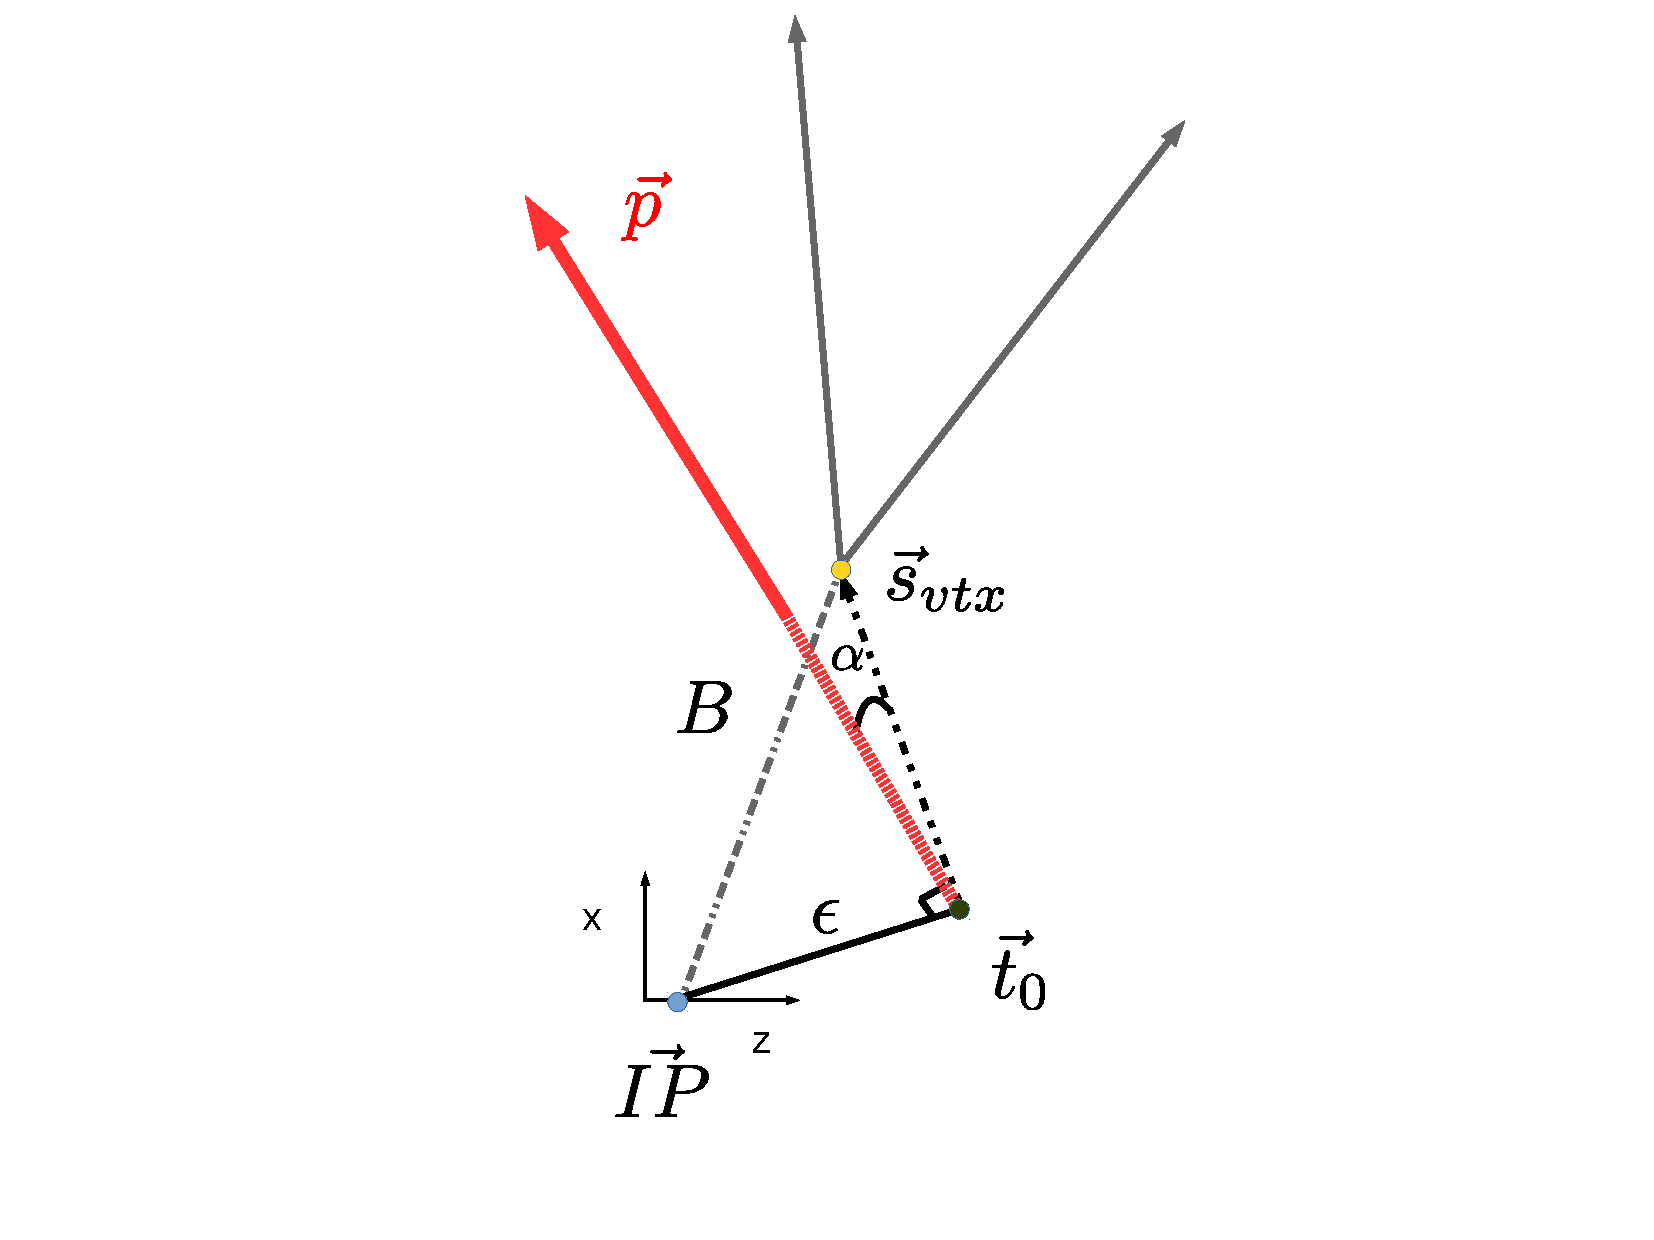
\includegraphics[width=0.75\textwidth]{ILD/plots/recovery-graph.pdf}
    \caption{\sl Illustration of the chosen separation variables of the vertex charge recovery algorithm, where $\vec{p}$ is a vector of a given particle momentum, $B$ is a flight distance of a b-hadron, $\vec{IP}$ is a primary vertex position, $\vec{t}$ is a reference point of a given particle, defined in \cite{bib:LCIOtrack}, $\alpha$ is the angle between $\vec{p}$ and $\vec{s}$ and $\epsilon$ is an offset distance of the particle. %Right: Same comparison, but after a cut on the b-tag$> 0.8$ and a cut on the b-hadron momentum more than 20\,GeV. The diagonal contains 55\% of the jets after the cuts.
    }
    \label{fig:VtxRecovery_3}
  }
\end{figure}

An algorithm, called VertexChargeRecovery, was developed to increase the jet charge purity by adding the missing prongs to the reconstructed vertices.  For a given jet, which has at least one associated reconstructed vertex, the VertexChargeRecovery has the following procedure:

\begin{itemize}
\item Preparation of the prong candidates - the algorithm uses all charged particles within a given jet as prong candidates. To recover the prongs, which has no reconstructed PFO, the program iterates throughout all reconstructed tracks and reconstructs them as charged PFOs without an associated calorimeter cluster. These new Particle Flow particles are used only if they have no duplicates in the previously selected jet particles;
\item All prong candidates are compared to the reconstructed prongs to avoid duplicates;
\item The separation variables $\alpha$ and $\epsilon$ are calculated for each prong candidate and a given reconstructed vertex;
\item The selection condition can be defined using the $\alpha$ and $\epsilon$ distributions for true b-hadron prongs and background particles, which are displayed in Fig.~\ref{fig:RecoveryPurity_3}. The standard condition is
\begin{equation}
\epsilon/\sigma > 2 + 25\cdot\alpha\text{ and } \alpha < 0.08.
\end{equation}
The recovery algorithm might have different behavior in simulation, than in real experiment, therefore, one should use a data-driven charge purity measurements, described in Sec.~\ref{sec:ChargePurity}, to test and tune the recovery parameters.
\item The algorithm creates new reconstructed vertices with old and recovered reconstructed prongs and links them to a given jet.
\end{itemize}

\begin{figure}[h]
{\centering
    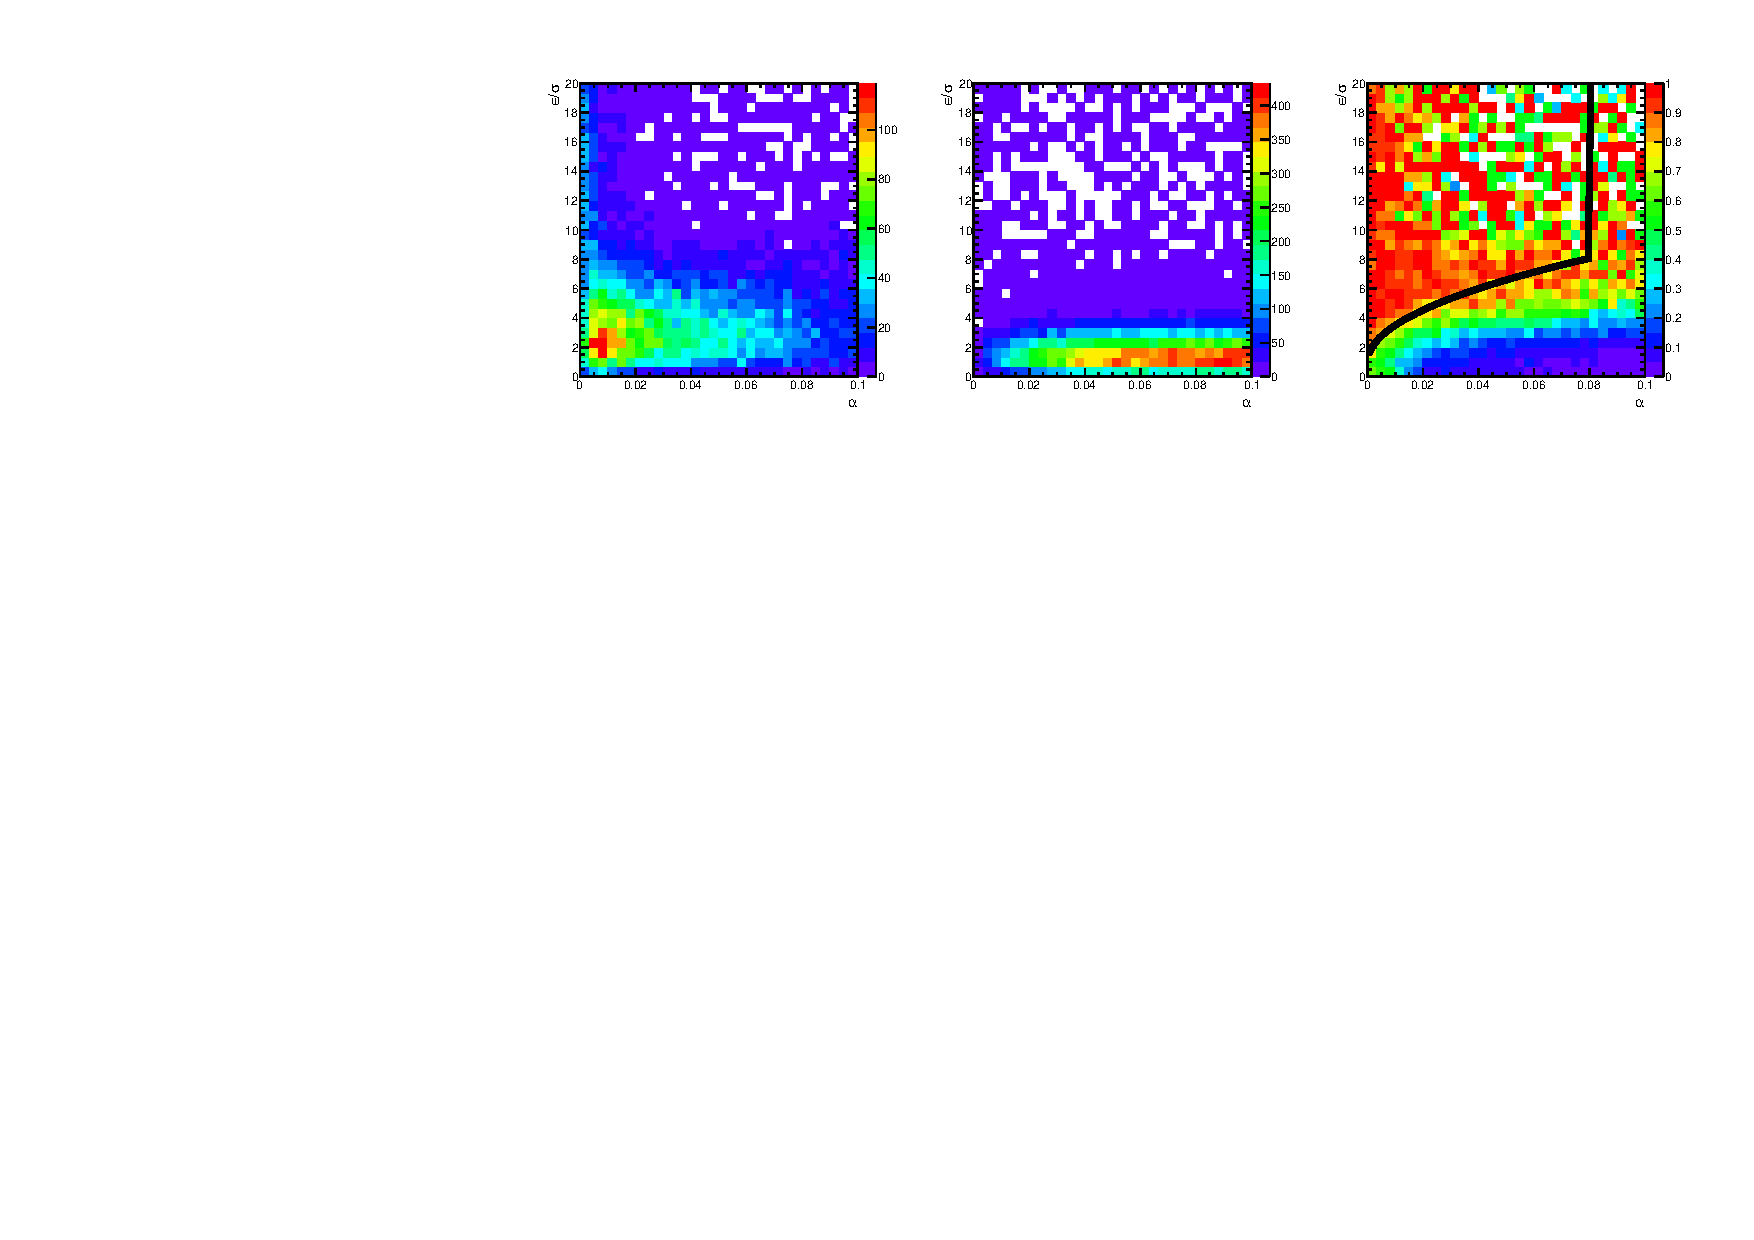
\includegraphics[width=0.95\textwidth]{ILD/plots/recovery-purity.pdf}
    \caption{\sl Distribution of the separation variables, the angle $\alpha$ and the offset significance $\epsilon/\sigma$ for the missing generated prongs and the background charged particles. Purity map shows the highest concentration of the missing generated prongs as compare to all charged particles. The black line demonstrates a possible cut function. %Right: Same comparison, but after a cut on the b-tag$> 0.8$ and a cut on the b-hadron momentum more than 20\,GeV. The diagonal contains 55\% of the jets after the cuts.
    }
    \label{fig:RecoveryPurity_3}
  }
\end{figure}


Hence, VertexChargeRecovery is made to have an output, identical to the output of the LCFI+ algorithms, which allows for a clear comparison of the jet charge reconstruction performance before and after vertex recovery usage.
%%%%%%%%%%%%%%%%%%%%%%%%%%%%%%%%%%%%%%%%%%%
%%%%%%%%%%%%%%%%%%%%%%%%%%%%%%%%%%%%%%%%%%%
%%%%%%%%%%%%%%%%%%%%%%%%%%%%%%%%%%%%%%%%%%%
\subsubsection{Results of the vertex recovery}

The simple algorithm of the vertex recovery is limited by the requirement of the presence of a reconstructed vertex and the reconstruction quality of a missing b-hadron prong. 
Nevertheless, this algorithm makes a significant improvement in the vertex reconstruction and the jet charge purity.

\begin{figure}[h]
{\centering
    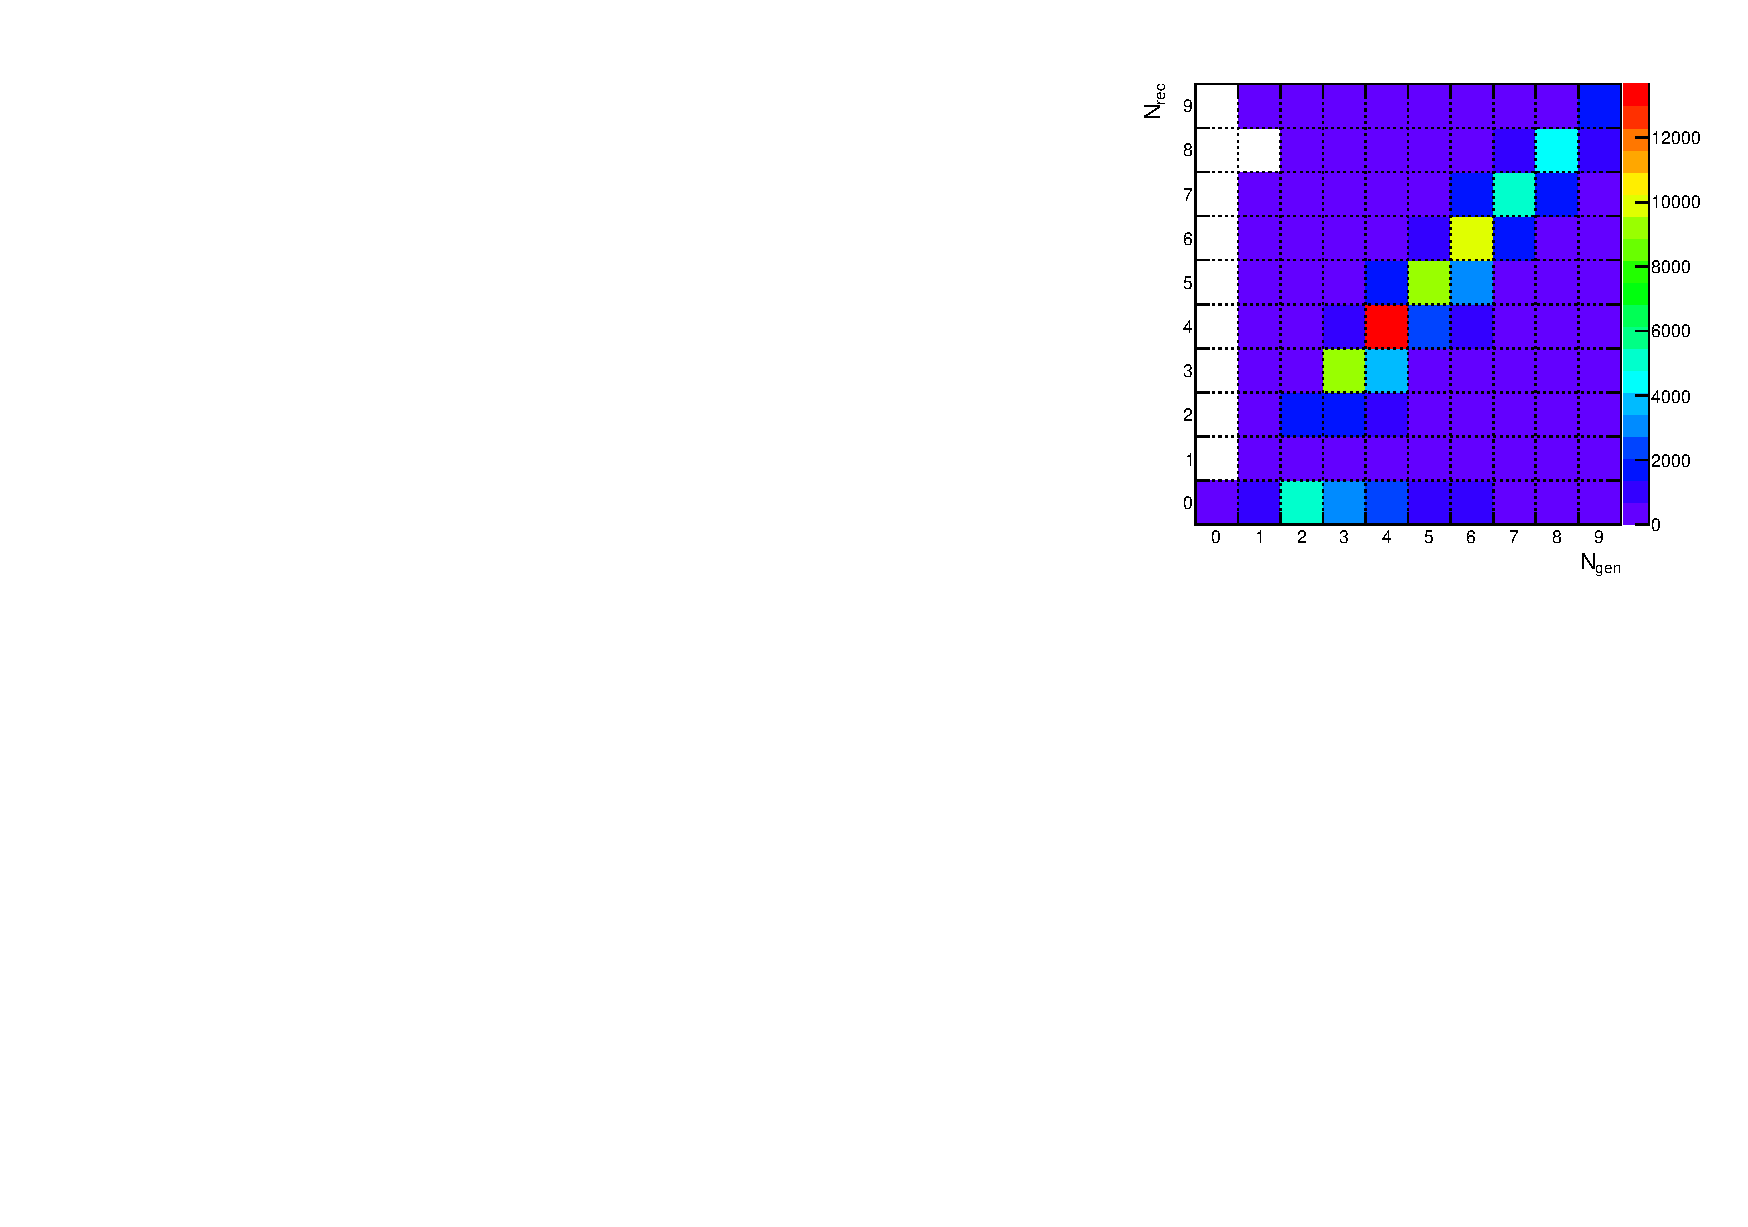
\includegraphics[width=0.55\textwidth]{ILD/plots/recovery-table.pdf}
    \caption{\sl Comparison of the number of reconstructed tracks $N_{gen}$ to the number of generated tracks $N_{rec}$ for a given b-jet after vertex charge recovery. The number of entries is color-coded for each cell. The fraction of the diagonal elements, which have the perfectly reconstructed vertices, is 62\% of all entries. The b-jets below diagonal have vertices with one or more particles missed by reconstruction. The row $N_{rec} = 0$ corresponds to the b-jets with no reconstructed vertices. %Right: Same comparison, but after a cut on the b-tag$> 0.8$ and a cut on the b-hadron momentum more than 20\,GeV. The diagonal contains 55\% of the jets after the cuts.
    }
    \label{fig:RecoveryTable_3}
  }
\end{figure}


The VertexChargeRecovery increases the fraction of correctly reconstructed jets from 49\% to 62\%, as it is illustrated in Fig.~\ref{fig:RecoveryTable_3}. 
This improvement is done by reducing the fraction of jets with $N_{rec} < N_{gen}$, below diagonal in Fig.~\ref{fig:RecoveryTable_3}. 
The slightly increased rate of jets with $N_{rec} > N_{gen}$ can be seen, which is an unavoidable shortcoming of the algorithm. 



\begin{figure}[h]
\centering
\begin{subfigure}{0.5\textwidth}
    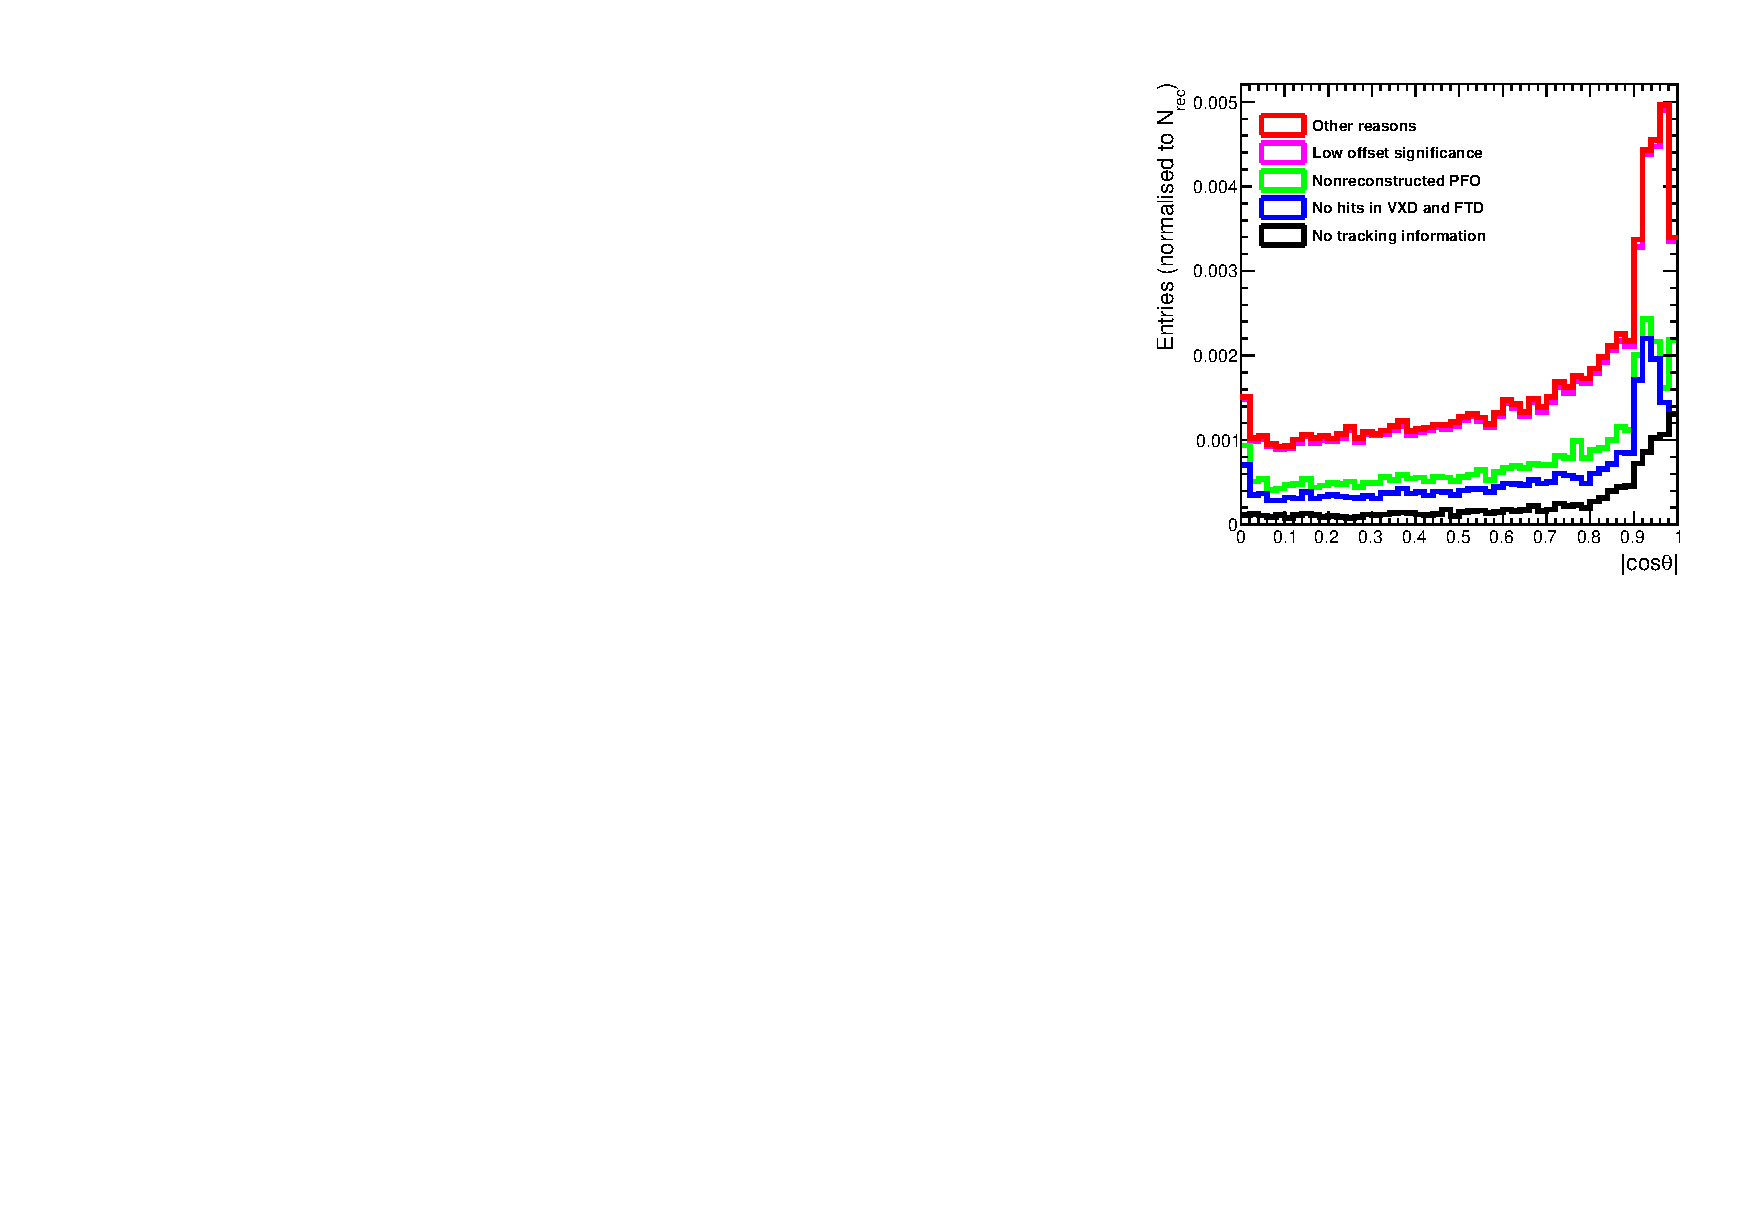
\includegraphics[width=0.95\textwidth]{ILD/plots/recovery-missed-cos.pdf}
\caption{\label{fig:RecoveryMissingTracks_cos_3} }
\end{subfigure}% 
  \begin{subfigure}{0.5\textwidth}
\centering
    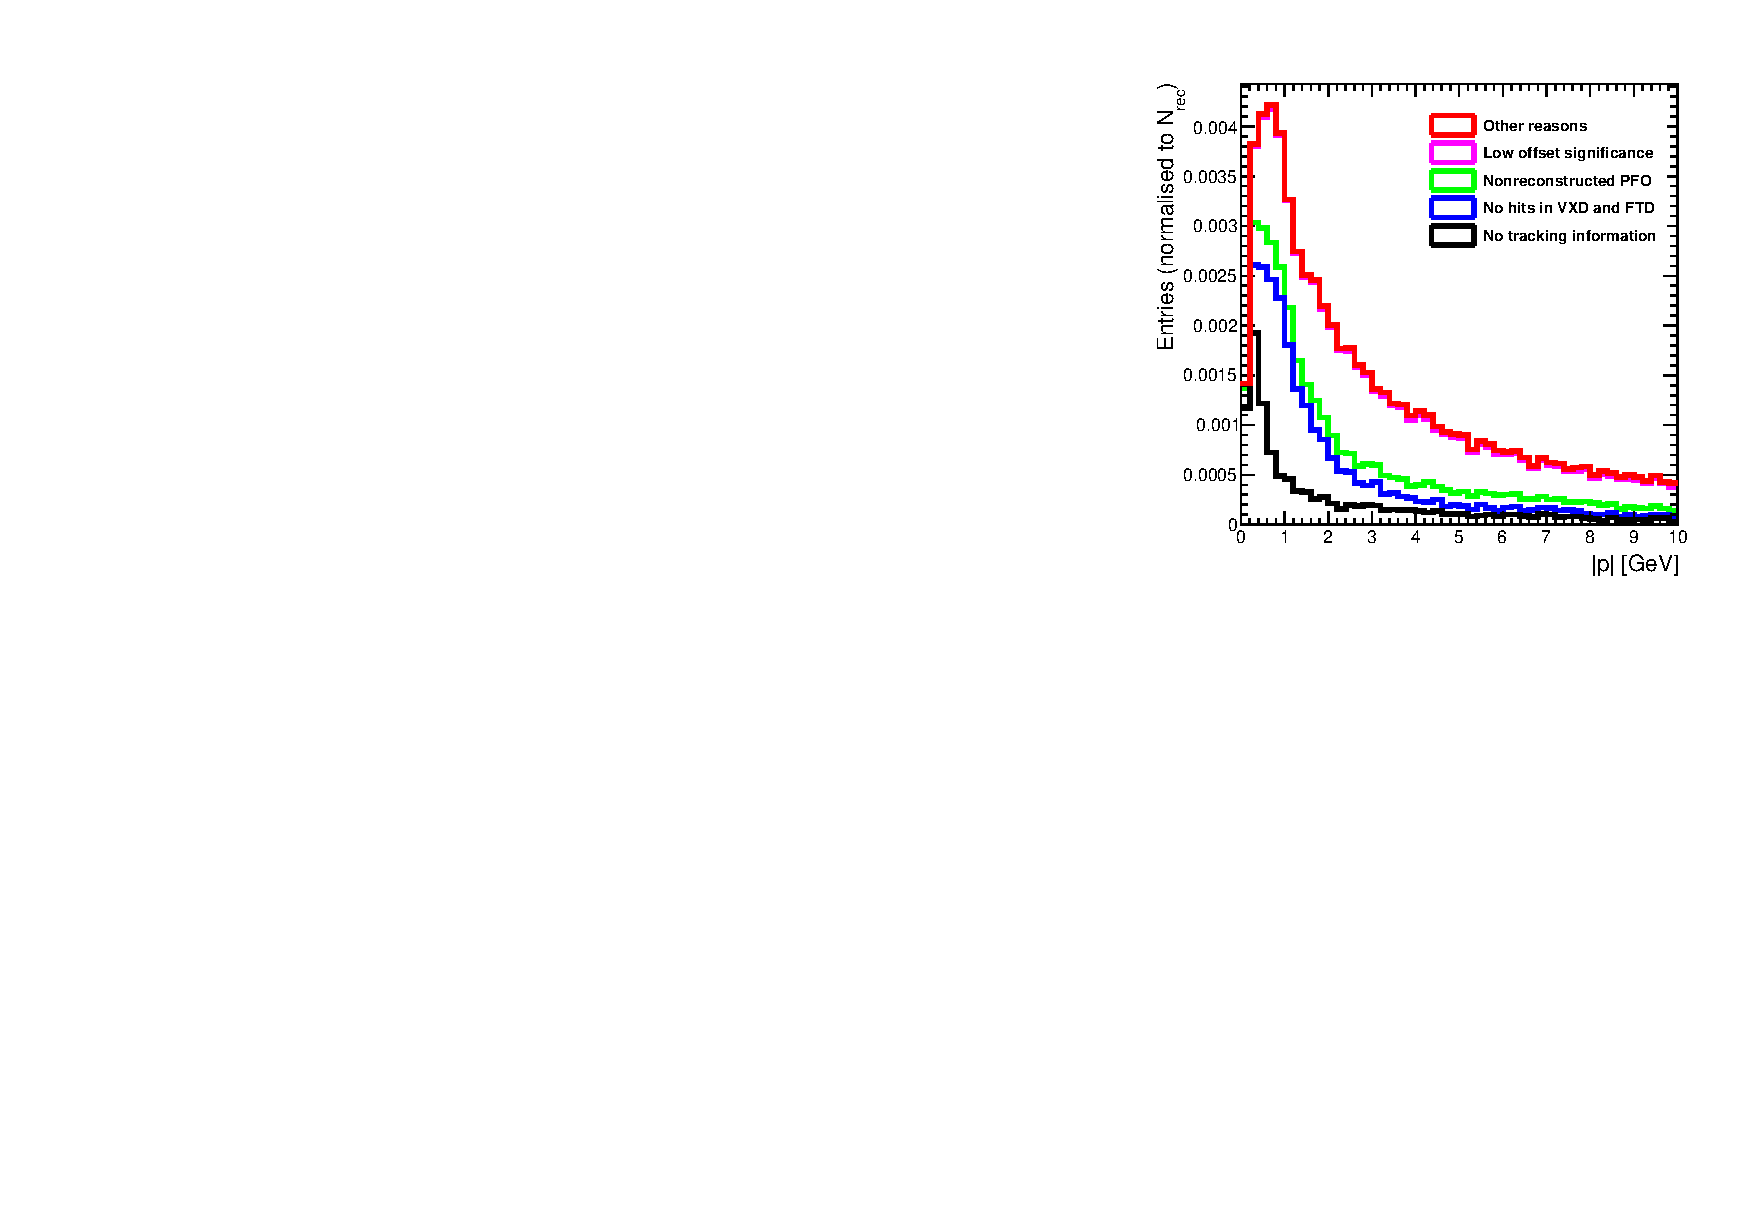
\includegraphics[width=0.95\textwidth]{ILD/plots/recovery-missed-p.pdf}
\caption{\label{fig:RecoveryMissingTracks_p_3} }
\end{subfigure}
    \caption{\sl Polar angle~(a) and momentum~(b) distributions of the missing prongs after vertex charge recovery subdivided into different categories. These are stacked histograms. }
    \label{fig:RecoveryMissingTracks_3}
\end{figure}

The vertex recovery decreases the fraction of missing prongs from 10.4\% to 6.2\%. The new polar angle and momentum distributions are shown in Fig.~\ref{fig:RecoveryMissingTracks_3}, from which one can see the following changes:
\begin{itemize}
\item The algorithm does not changes the categories of b-hadron prongs, which have no reconstructed tracks;
\item The reconstructed prongs with no assigned VXD or FTD hits are not recovered by the program;
\item The most of the missing prongs, which have no corresponding PFO are successfully associated to the correct reconstructed vertices;
\item The large peak of the missing prongs at $|\cos\theta| \approx 0.8$ is successfully eliminated;
\item The prongs in the region of the strong background, as can be seen in Fig.~\ref{fig:RecoveryPurity_3}, are not used by the program;
\item The missing prongs, which where lost by other means, are successfully recovered by the algorithm.
\item The vertex recovery can use all particles, even the ones with a small momentum, below 1\,GeV or outside the barrel VXD acceptance. 
\end{itemize}

To resolve the inefficiencies, caused by the tracking, one can apply different VXD tracking algorithms, like minivector tracking. 

The central result of the algorithm is that it enhances the jet charge purity from 66\% to 73\%, despite increase of the contamination by the  background particles from 3\% to 4\%.
Figure~\ref{fig:RecoveryPurityComparison_3} demonstrates the improvement of the jet charge purity as function of the jet b-tag, reconstructed b-hadron momentum, $N_{rec}$ and the polar angle of the b-hadron  $|\cos\theta_{vtx}|$.
\begin{figure}[h]
{\centering
    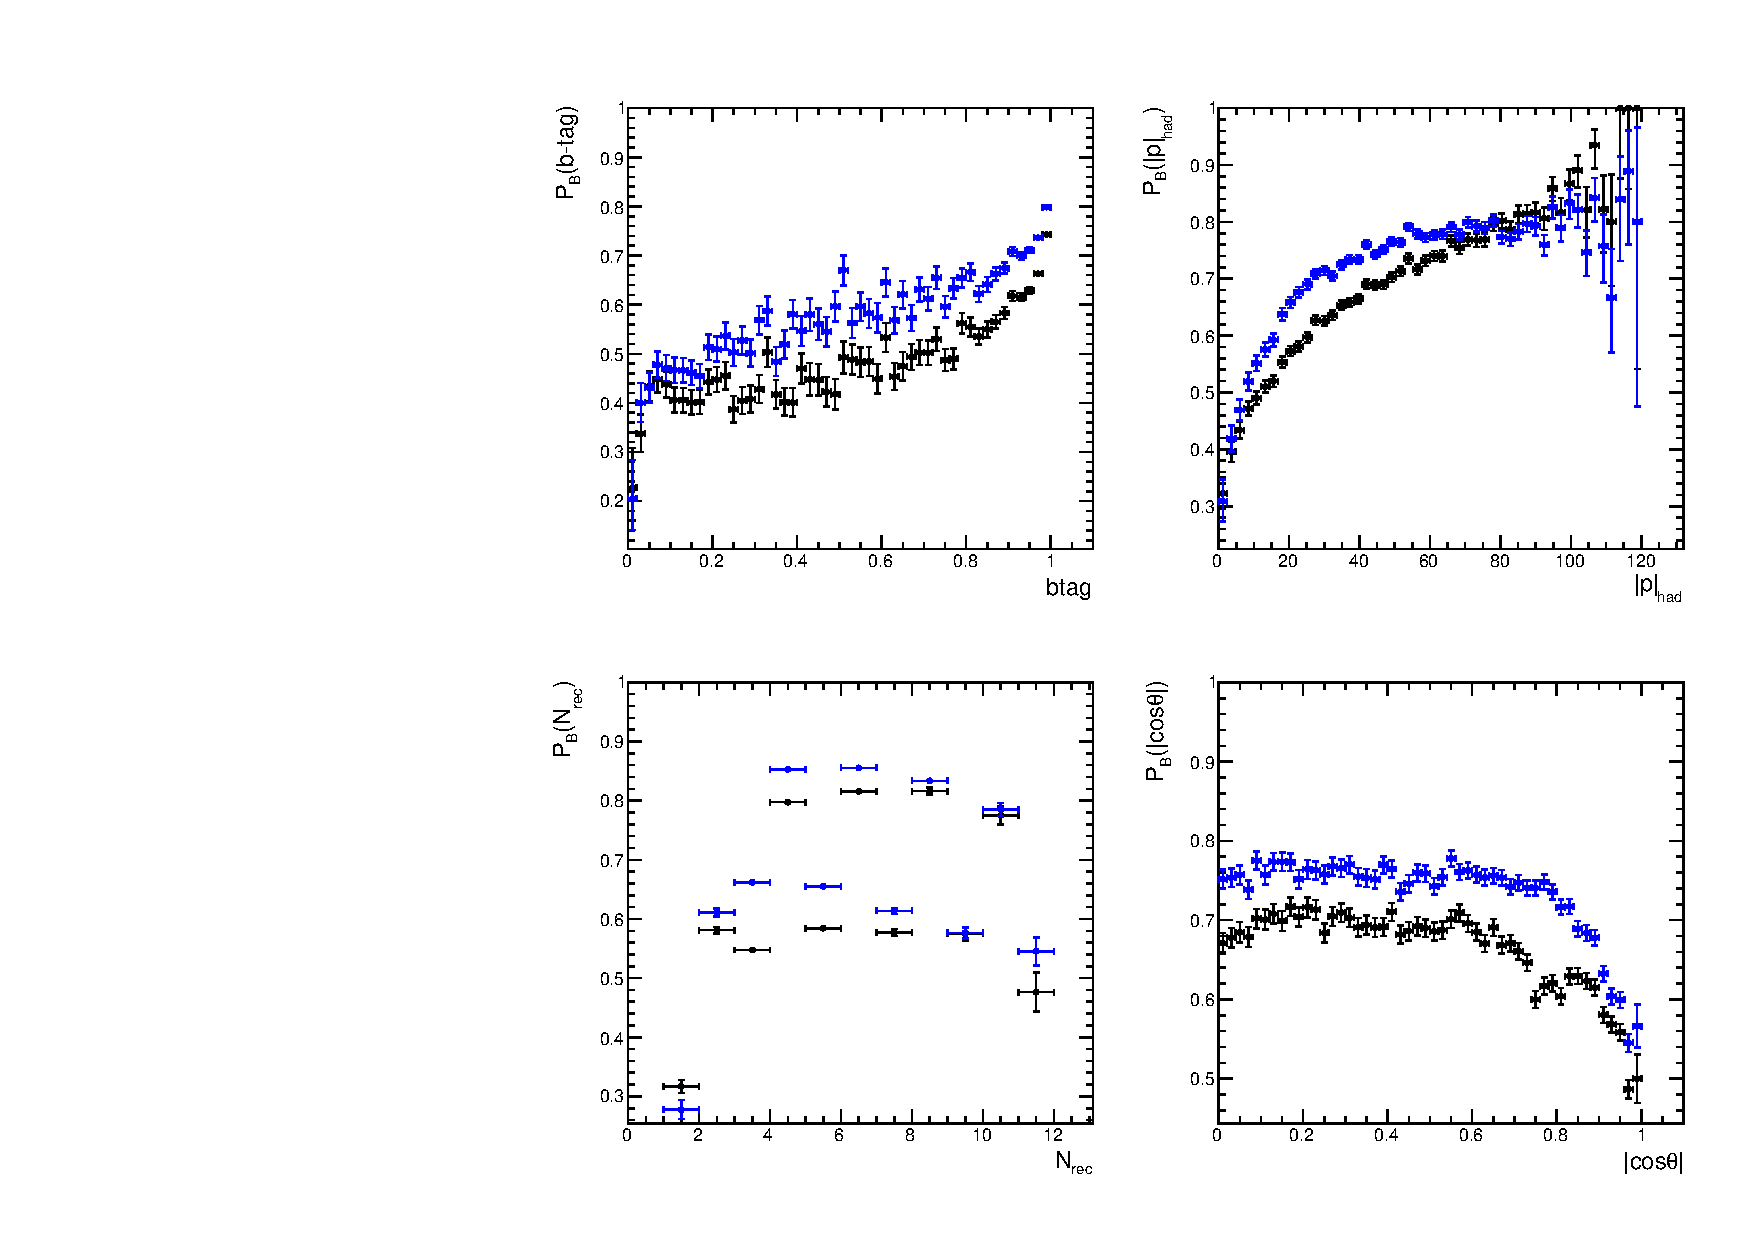
\includegraphics[width=0.95\textwidth]{ILD/plots/recovery-purity-comparison.pdf}
    \caption{\sl Comparison of the purity as function of the jet b-tag, reconstructed b-hadron momentum, $N_{rec}$ and the polar angle $|\cos\theta|$ before and after the vertex recovery algorithm.  
    }
    \label{fig:RecoveryPurityComparison_3}
  }
\end{figure}
One can see the following changes done by the recovery algorithm:
\begin{itemize}
\item Jets with a b-tag$>0.3$ have higher chances to be recovered. The b-tag value strongly depends on the offsets of the reconstructed prongs, the low b-tag jets have less significant offsets of particles, which makes them  harder to recover. 
\item The algorithm improves the jets with a moderate reconstructed b-hadron momentum. The algorithm should be tuned to work with highly collimated vertices produced by high momentum b-hadrons.
\item The large improvement can be seen to the jets or reconstructed b-hadrons with low number of reconstructed prongs, especially for $N_{rec}=3$. For higher multiplicity, the algorithm should recover all tracks correctly, which is not trivial. Hence, almost no improvement is seen for the reconstructed b-hadrons with large $N_{rec}$.
\item The algorithm is capable to increase the purity in the barrel VXD acceptance and restore the damage done by the non-reconstructed PFO particles at $|\cos\theta_{vtx}| \approx 0.8$. 
\end{itemize}
The jet charge purity can be also increased by applying cuts on the reconstructed observables up to 80\% purity with 60\% efficiency or by application of MVA algorithm.

To summarize, the VertexChargeRecovery is able to significantly improve the jet charge purity and equalize it in the polar angle spectrum, which is crucial for reconstruction of heavy quark differential cross section and forward-backward asymmetry. 
%%%%%%%%%%%%%%%%%%%%%%%%%%%%%%%%%%%%%%%%%%%
%%%%%%%%%%%%%%%%%%%%%%%%%%%%%%%%%%%%%%%%%%%
%%%%%%%%%%%%%%%%%%%%%%%%%%%%%%%%%%%%%%%%%%%
\subsection{Using the $dE/dx$ information}

An alternative method to measure the b-jet charge is to identify among the reconstructed b-hadron prongs the charged kaon $K^\pm$, which carry the information about the initial b-quark charge. 

The charged kaons have much higher mass than the charged pions and lower mass than protons, which give a possibility to identify charged kaons by the energy deposition of the hits in the subdetectors. 

The most suitable device to calculate the energy deposition per distance passed, the $dE/dx$ value, is the ILD TPC due to its continuous gaseous environment. 


The $dE/dx$ as a function of particle momentum and $|\cos\theta|$ for different hadrons is shown in Fig.~\ref{fig:dEdxBefore_3}. One can immediately spot the dependence of the $dE/dx$ value on the polar angle of the particles. This happens because of the knocked-out electron emittance or $\delta$-ray probability is increased with increasing length of the TPC track. Therefore, one needs to apply an angular correction to remove the angular dependence of the $dE/dx$ value, which is 
\begin{equation}
	\frac{dE}{dx}\to\frac{dE}{dx}\theta^{0.15},
    \label{formula:dEdxCorrection}
\end{equation}
where $\theta$ is the polar angle of the particle. 
This angular is known to be applied at other experiments, which have the TPC devices~\cite{bib:HARP}.

The distributions of the $dE/dx$ as a function of particle momentum and $|\cos\theta|$ after the angular correction (\ref{formula:dEdxCorrection}) are displayed in Fig.~\ref{fig:dEdxAfter_3}.
\begin{figure}[h]
{\centering
    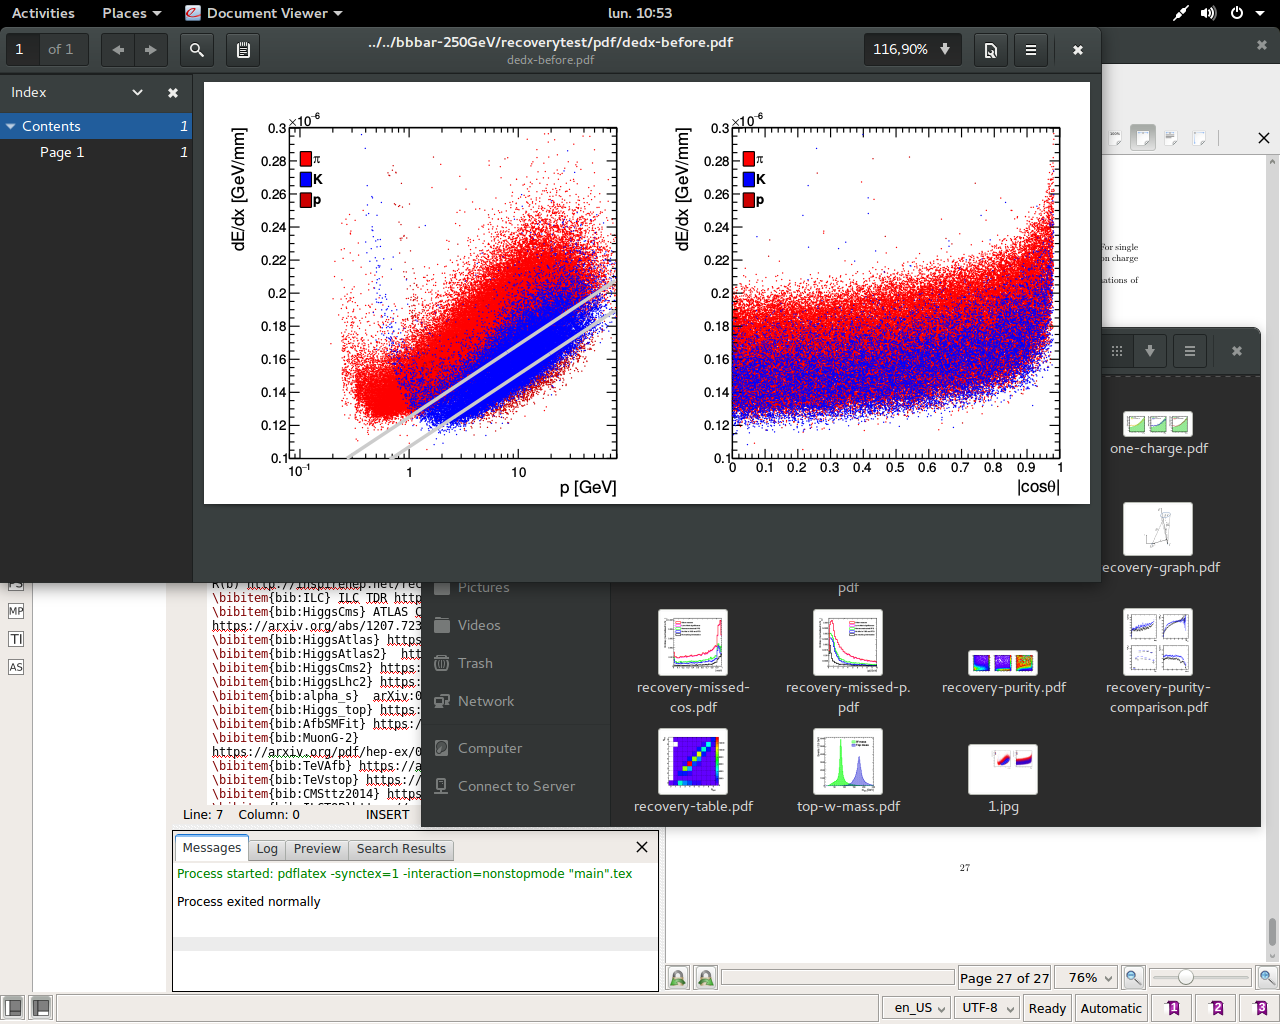
\includegraphics[width=0.95\textwidth]{ILD/plots/dedx-before.pdf}
    \caption{\sl The energy deposition per track length $dE/dx$ as function of the particle momentum, the particle polar angle $|\cos\theta|$ for different particles. Two gray lines separate out the region with a maximal kaon concentration. 
    }
    \label{fig:dEdxBefore_3}
  }
\end{figure}

\begin{figure}[h]
{\centering
    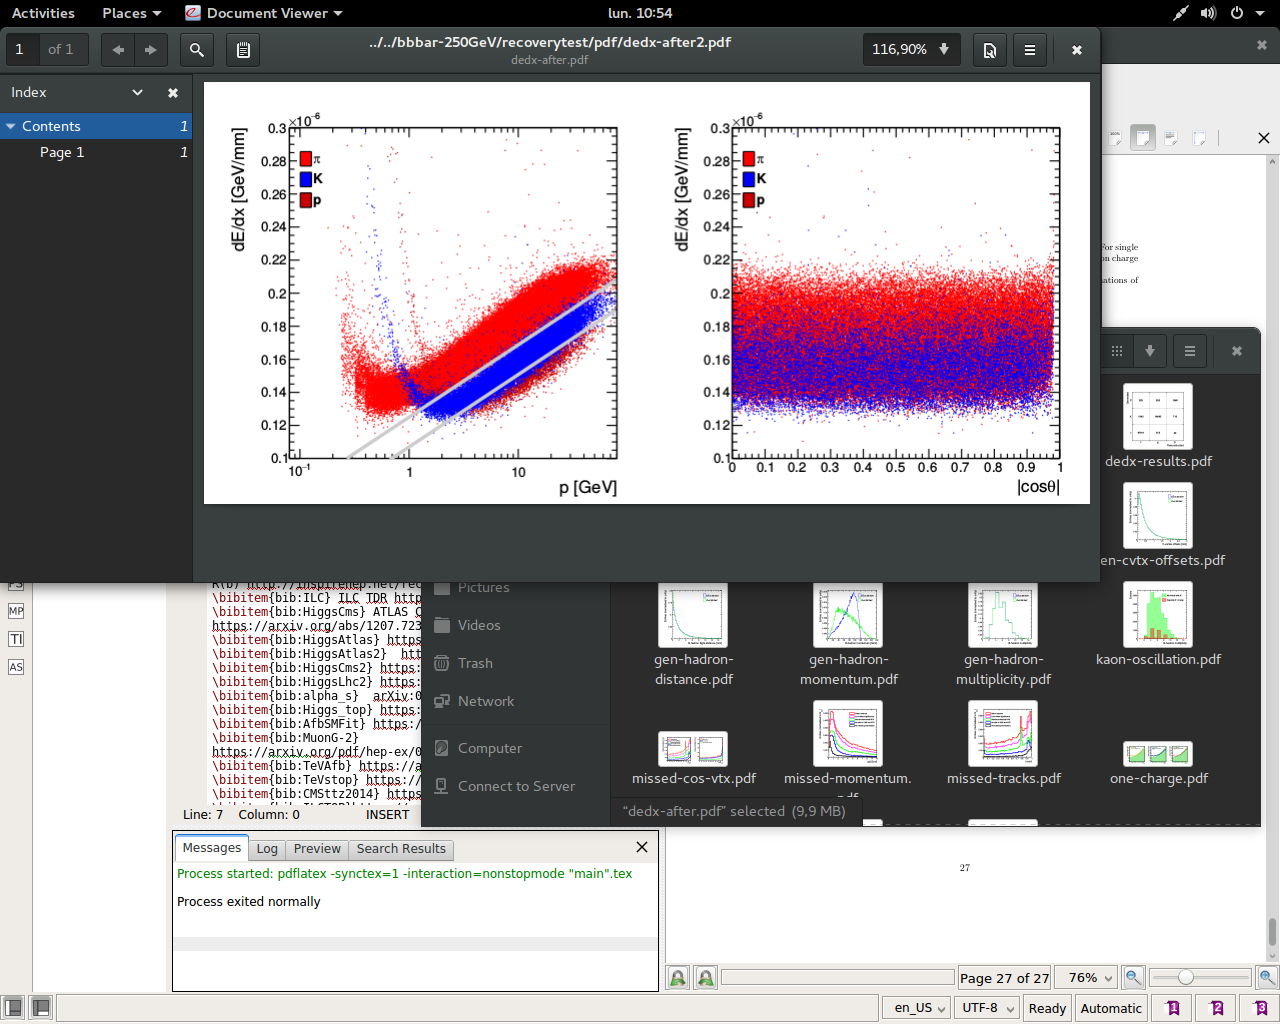
\includegraphics[width=0.95\textwidth]{ILD/plots/dedx-after.pdf}
    \caption{\sl The energy deposition per track length $dE/dx$ as function of the particle momentum, the particle polar angle $|\cos\theta|$ for different particles after application of the angular correction, described in text. Two gray lines separate out the region with a maximal kaon concentration. 
    }
    \label{fig:dEdxAfter_3}
  }
\end{figure}

A simple cut-based algorithm was developed to identify the particle type (PID) using $dE/dx$ information after angular correction, which can identify kaons with 97.\% purity and 87.7\% efficiency.
The results of the hadron identification are displayed in Fig.~\ref{fig:dEdxResults_3}.

The angular correction is now included in the latest version of the {\sc ilcsoft} distribution.

\begin{figure}[h]
{\centering
    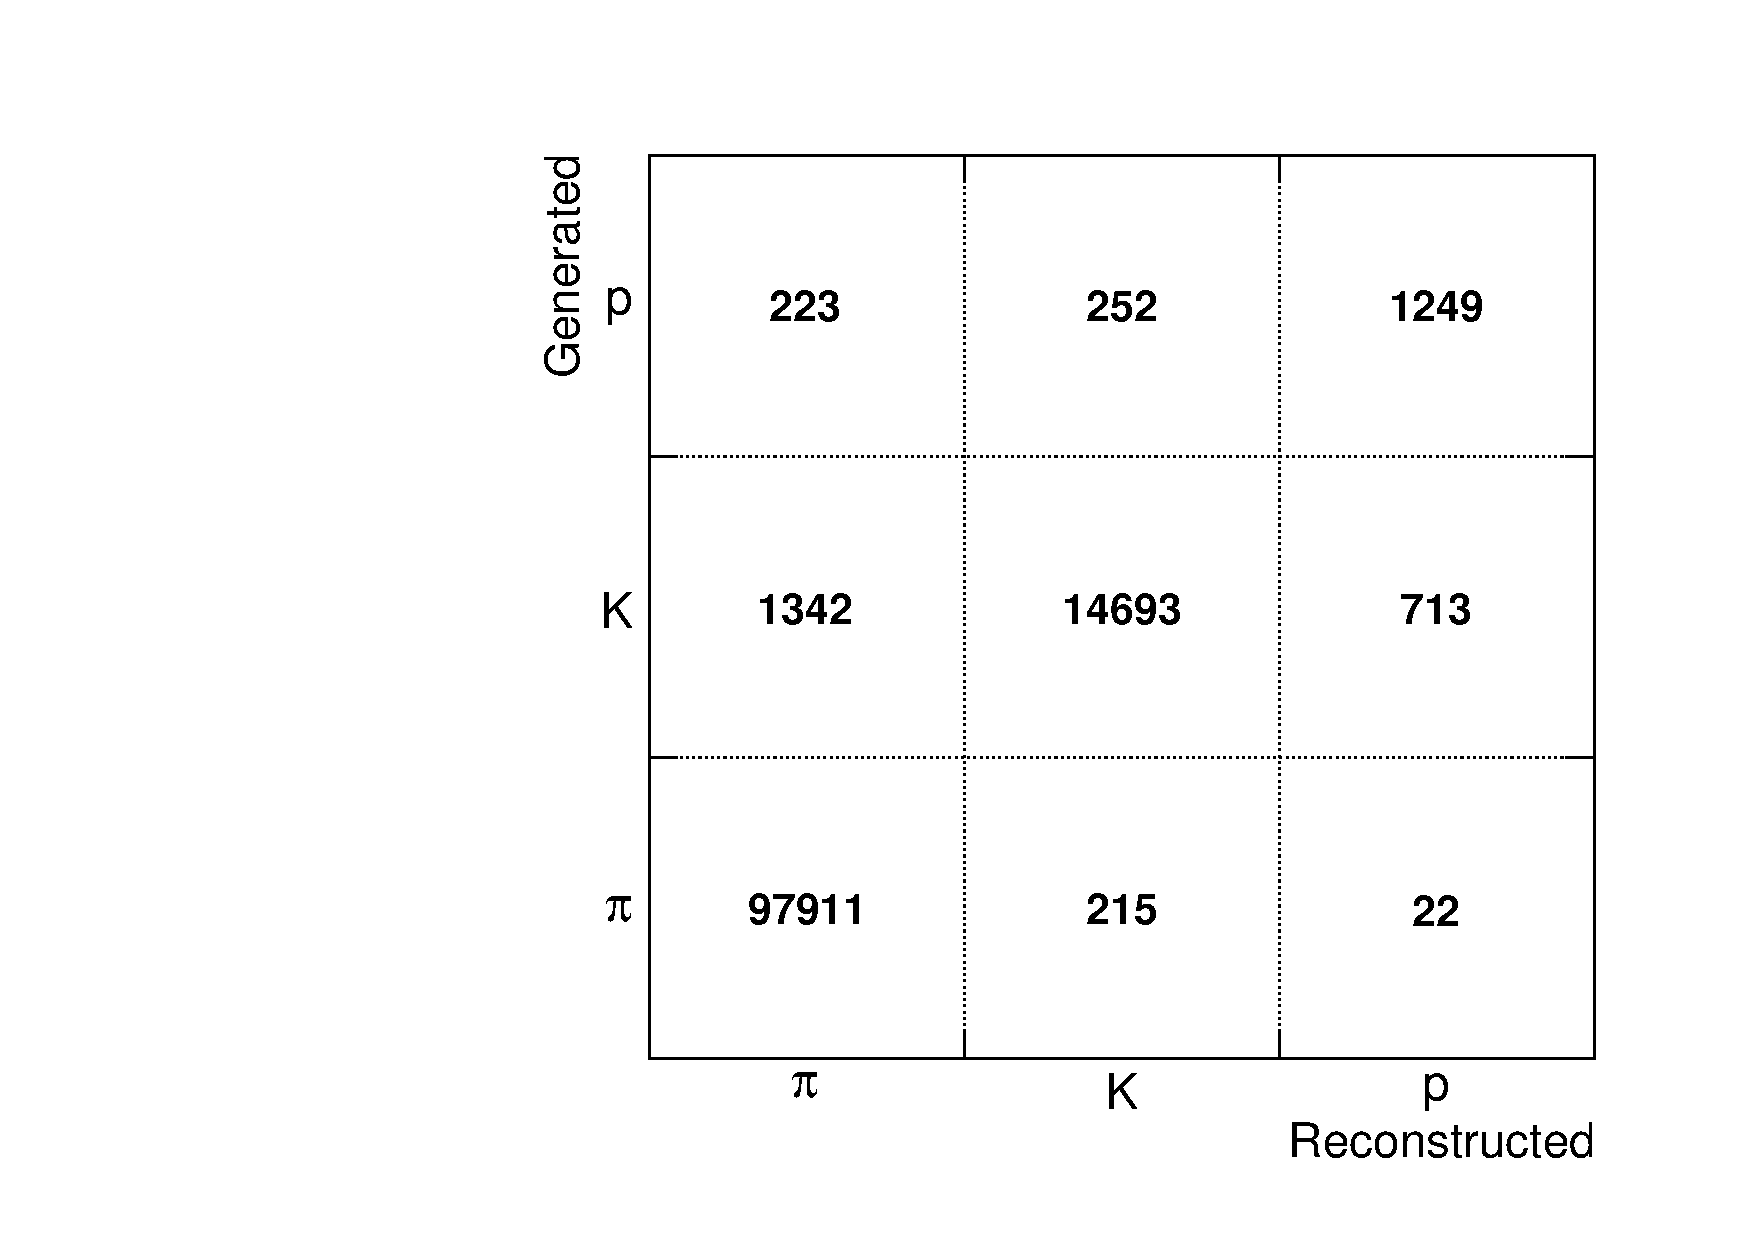
\includegraphics[width=0.45\textwidth]{ILD/plots/dedx-results.pdf}
    \caption{\sl Correlation histogram between generated particle type and reconstructed particle type produced by the cut-based PID algorithm.
    }
    \label{fig:dEdxResults_3}
  }
 
\end{figure}


Given the reconstruction purity illustrated in Fig.~\ref{fig:dEdxResults_3} and the correlation between kaon charge and the b-hadron charge in Fig.~\ref{fig:KaonOscillation_3}, one can conclude that the reconstructed charged kaons from the reconstructed vertices provide a reliable information on the charge of the initial b-hadron or b-quark. 
%%%%%%%%%%%%%%%%%%%%%%%%%%%%%%%%%%%%%%%%%%%%%%%%%%%%%%%%%
%%%%%%%%%%%%%%%%%%%%%%%%%%%%%%%%%%%%%%%%%%%%%%%%%%%%%%%%%
%%%%%%%%%%%%%%%%%%%%%%%%%%%%%%%%%%%%%%%%%%%%%%%%%%%%%%%%%


\section{Top quark production at the ILC}
%Direct electroweak production of the top quark pairs
This section of the thesis describes an application of the jet charge measurement technique, described in Sec.~\ref{sec:JetChargeReconstruction}, to the forward-backward asymmetry measurement for $e^+e^- \to t\bar{t}$ process at ILC, which is used to determine the electroweak couplings of the top quark.

The measurements of the top quark properties is one of the key points of the \sm\ physics program at the ILC.

\subsubsection{Properties of the top quark}

The top quark is the heaviest elementary particle in the \sm\ with measured mass of 173.34$\pm$0.27(stat)$\pm$0.71(syst) \,GeV~\cite{bib:TopMass}, which implies a very short lifetime of approximately 5$\cdot10^{-25}$\,s.
The top quark lifetime is short comparing to a time needed for hadronization process  (10$^{-23}$\,s), therefore, the top quark decays too fast to form hadrons. 
This fact permits to study the bare quark properties, like spin, via its decay particles. 

The dominant decay mode of the top quark is $t\to bW^+$, which is 99.8\% of all top decays, the $W^\pm$ boson can decay to a lepton-neutrino pair or to a quark pair, which implies a six fermion final state of the $e^+e^-\to t\bar{t}$ process.
The $t\bar{t}$  decays are classified by the $W^\pm$ decay modes:
\begin{itemize}
	\item Fully hadronic decay $t\bar{t} \to bq\bar{q} \bar{b} q\bar{q}$ -  46.2\% of branching ratio;
	\item Semileptonic decay $t\bar{t} \to bq\bar{q} \bar{b} l\nu_l$ - 43.5\% of branching ratio;
	\item Fully leptonic decay $t\bar{t} \to b l^- \nu_{l^-} \bar{b} l^+\nu_{l^+}$ - 10.3\% of branching ratio.	
\end{itemize}

At the ILC it is possible to reconstruct and study all decay modes of the $t\bar{t}$ pair.
%%%%%%%%%%%%%%%%%%%%%%%%%%%%%%%%%%%%%%%%%%%%%%%%%%%%%%%%%
%%%%%%%%%%%%%%%%%%%%%%%%%%%%%%%%%%%%%%%%%%%%%%%%%%%%%%%%%
%%%%%%%%%%%%%%%%%%%%%%%%%%%%%%%%%%%%%%%%%%%%%%%%%%%%%%%%%
\subsection{Setup of the study}
%The top quark pairs at the ILC can be produced at $\sqrt{s}=350$\,GeV and 500\,GeV. 
In this section of the thesis, the semileptonic $t\bar{t}$ pairs produced at $\sqrt{s}=500$\,GeV are studied using full ILD simulation.
The chosen center-of-mass energy allows for top pair production free from $t\bar{t}$ threshold QCD effects.
The cross sections at the Born level of the signal process $e^+e^- \to t\bar{t}$ and the major \small\ background processes at the $\sqrt{s} = 500$\,GeV are summarized in Table~\ref{table:ttbarsigma}.

The clear process signature of two b-jets, two light jets and an isolated lepton makes the semileptonic decay mode easily reconstructable and usable for forward-backward asymmetry measurement. 
This choice also allows for a direct comparison and combination of the new results obtained by the b-jet charge measurement technique with previous studies done using $W^\pm$ lepton charge method~\cite{bib:ILCTOP}.

This thesis concentrates on the left-handed electron polarization case, because of lepton migration problem caused by the $W^\pm$ kinematics.
%The setup of the 
%The large production cross section
%The 350 GeV threshold mass scan 
%The 500 GeV coupling 

%\subsection{Top quark decay modes}

\subsection{Top quark reconstruction}
In this thesis, the top reconstruction method, which was developed for~\cite{bib:ILCTOP} is applied, which has the following steps:
\begin{itemize}
	\item Isolated lepton identification is done using LAL LeptonFinder algorithm~\cite{bib:Doublet}, which is designed to find an energetic lepton or a lepton, which has a significant transverse momentum with respect to the neighbored jets. 
	\item The events, after excluding the isolated lepton, are clustered to four jets using Durham jet clustering algorithm.
	\item The b-jet tagging done by LCFI+ is used to identify the two b-jets. 
	\item The last step of the top reconstruction is to associate one of the b-jets with the two light jets, which come from the hadronic $W^\pm$ decay.  One has two possibilities to combine the jets and one can choose the best combination using minimization of the following expression:
	\begin{equation}
	\label{formula:Chi2Top_3}
	d^2_{t} = (\frac{m_{cand}-m_{t}}{\sigma_{m_t}})^2 + (\frac{E_{cand}-E_{beam}}{\sigma_{E_{beam}}})^2+(\frac{p^*_b-68\,GeV}{\sigma_{p^*_b}})^2 + (\frac{\cos\theta_{bW}-0.23}{\sigma_{\cos\theta_{bW}}})^2,
	\end{equation}
	where $m_{cand}$ and $E_{cand}$ are the invariant mass and the energy of the top quark candidate, $m_t$ and $E_{beam}$ are the input top quark mass and the nominal beam energy of 250\,GeV, $p^*_b$ is the momentum of the b quarks in the top quark frame with nominal value of 68\,GeV and $\cos\theta_{bW}$ is the angle between the b quark and the $W^\pm$ boson with a nominal value of 0.23.
\end{itemize}

The reconstructed distributions of the top and $W^\pm$ invariant masses are shown in Fig.~\ref{fig:TopWmass_3}, which is an illustration of the reconstruction flo

\begin{figure}[h]
	{\centering
		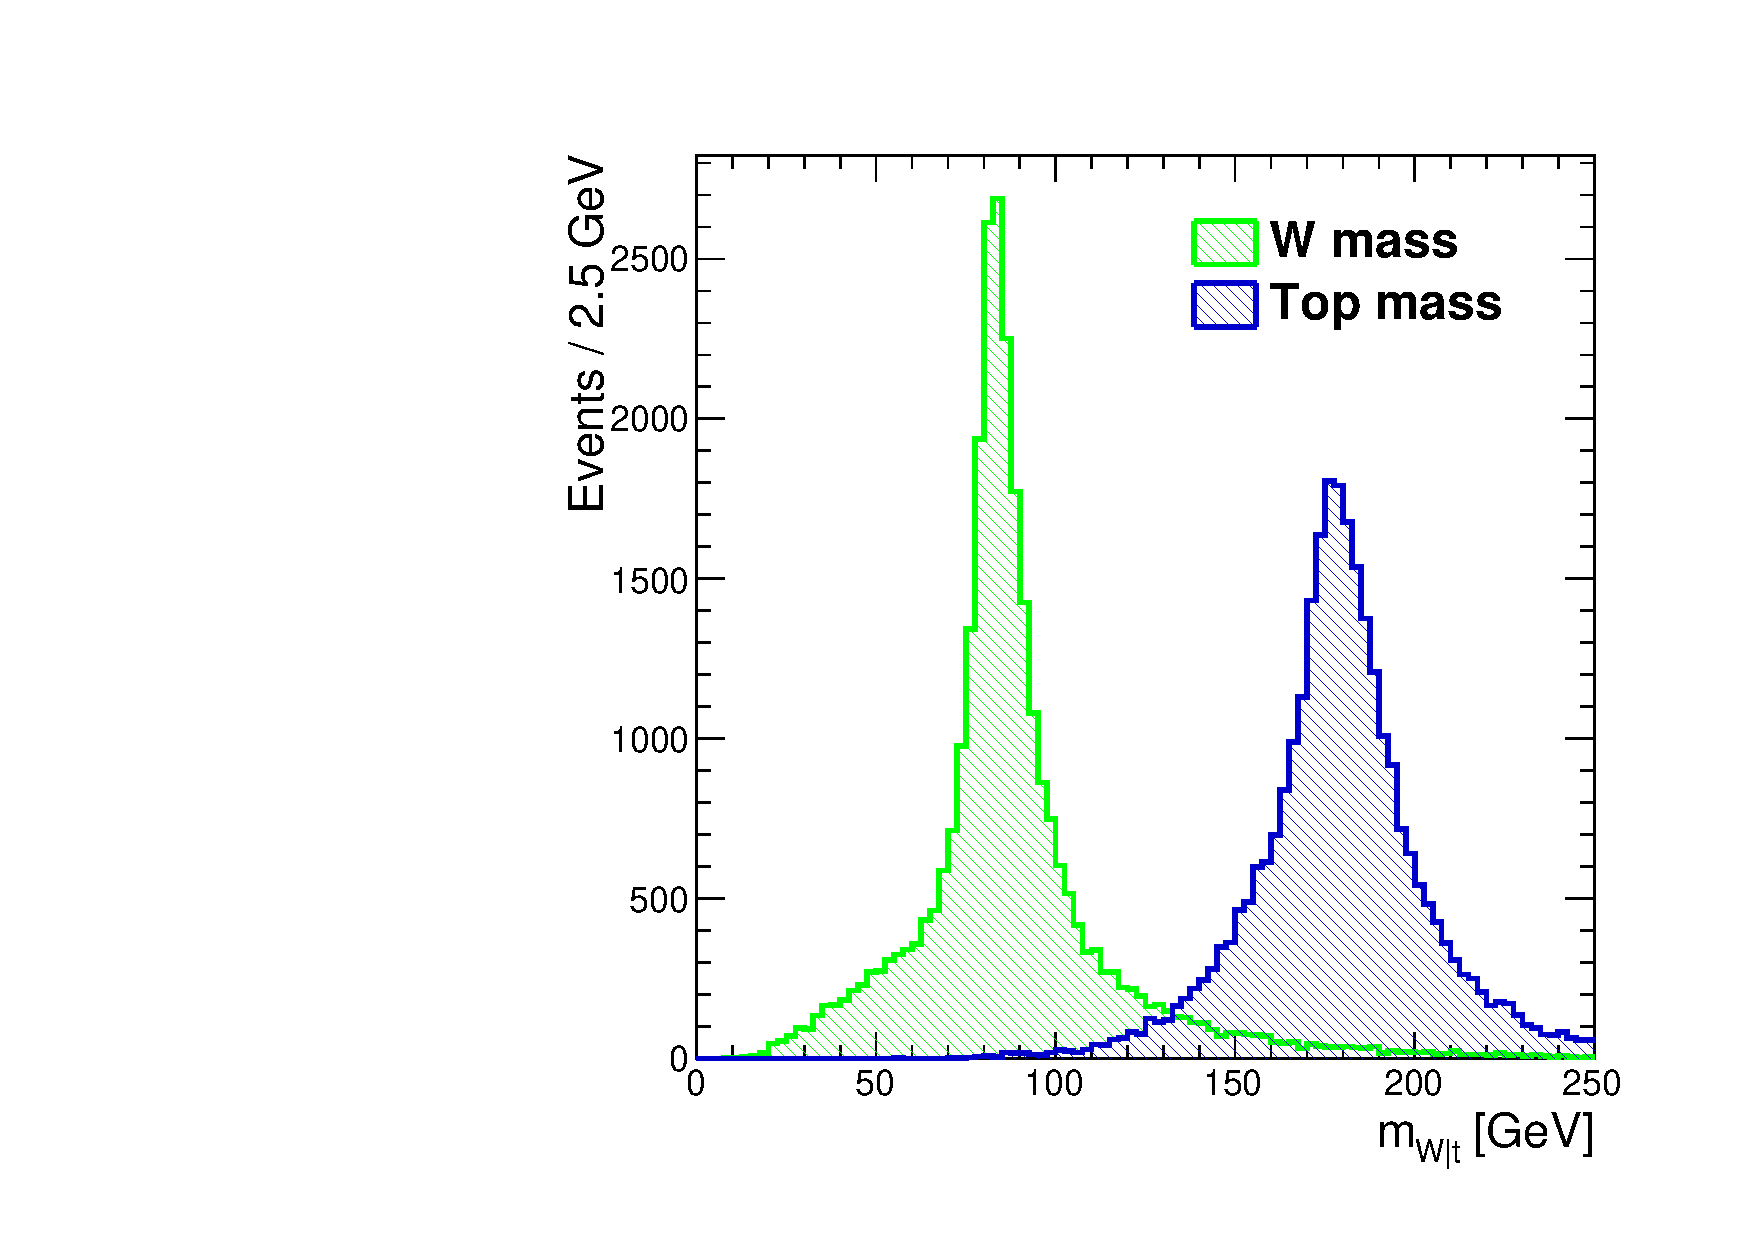
\includegraphics[width=0.55\textwidth]{ILD/plots/top-w-mass.pdf}
		\caption{\sl Reconstructed invariant mass distributions of the hadronic top quark and hadronic $W^\pm$ boson decays.
		}
		\label{fig:TopWmass_3}
	}
	
\end{figure}

\subsection{Background processes}
The main background processes are summarized in Table~\ref{table:ttbarsigma}. 
The previous studies~\cite{bib:ILCTOP}\cite{bib:Doublet} shown that the major backgrounds to the semileptonic \ttbar\ decay are the single top process and fully hadronic of fully leptonic \ttbar\ decays. 
%Several \sm\ processes give a rise to the six fermion final state, 
        \begin{table}[H]
        \begin{center}
        \begin{tabular}{l c c c}
        \hline
	Channel & $\sigma_{unpol.}$\ [fb] & $\sigma_{LR}$ [fb] &  $\sigma_{LR}$ [fb] \\
	\hline
	$t\bar{t}$ & 572 & 1564 & 724 \\
	$\mu\mu$ & 456 & 969 & 854 \\
	$uu + cc + ss + dd$ & 2208 & 6032 & 2793 \\
	$b\bar{b}$ & 372 & 1212 & 276 \\
	$\gamma Z^0$ & 11185 & 25500 & 19126 \\
	$WW$ & 6603 & 26000 & 150 \\ 
	$Z^0Z^0$ & 422 & 1106 & 582 \\
	$Z^0WW$ & 40 & 151 & 8.7 \\
	$Z^0 Z^0 Z^0$ & 1.1 & 3.2 & 1.22 \\
        \hline
        \end{tabular}
        \end{center}
        \caption{\sl Unpolarized and 100\% polarized cross sections at the Born level for signal and background processes at $\sqrt{s}=500$\,GeV~\cite{bib:ILCTOP}. }
        \label{table:ttbarsigma}
        \end{table}


One can use the kinematical cuts to suppress background processes from~\cite{bib:Doublet}:
\subsection{Results}


\section{Bottom quark production at the ILC}

\subsection{Bottom quark reconstruction}
\subsection{Charge purity measurement}
\label{sec:ChargePurity}
\subsection{Corrections to the polar angle}
\subsection{Background processes}
\subsection{Results}

\section*{Conclusions}